\chapter{Deanonymization of transactions with network analysis}

\label{Chapter03Clustering}

In this Chapter, we describe a novel network-level deanonymization attack on cryptocurrencies.\footnote{This Chapter is based on~\cite{Biryukov2019a, Biryukov2019b}. This work was partially supported by the Zcash Foundation grant 2017Q4-24~\cite{Feher2017}.}
We show how a global passive adversary can cluster transactions issued from the same node and correlate the clusters with IP addresses.

Our method is based on analyzing the timings of transaction announcements.
We, as the authors of~\cite{Biryukov2014}, go beyond the first relayer heuristic~\cite{Koshy2014} and consider multiple announcements for each transaction.
First, we collect the data using geographically distributed listening nodes.
We then apply carefully chosen weight functions to transaction announcement timestamps.
We observe that the weight vectors of transactions issued from the same node exhibit stronger correlations.
This technique allows us to cluster such transactions with high accuracy.
We also unpack address advertisement messages (\texttt{addr}), which may help link transaction clusters to IP addresses of the corresponding nodes under certain assumptions.

We test our method on Bitcoin and three privacy-focused cryptocurrencies.
We cluster our own transactions in the Bitcoin testnet and Zcash with high levels of precision and recall.
In particular, we can cluster Zcash transactions that involve both transparent and shielded addresses.
We estimate the cost of a full-scale attack on the Bitcoin mainnet at hundreds of US~dollars, feasible for a low budget adversary.
We also prove the applicability of our technique to Dash and Monero.

Our clustering method may act as a complement to transaction graph analysis.
The network-based analysis may reveal a relationship between transactions with no common public keys used in their inputs and outputs.
Analogously, transactions sharing some addresses may be announced though different sets of nodes.


\section{Transaction clustering with timing analysis}  \label{sec:Ch03Ourapproach}

Each transaction is initially introduced by a single peer -- the \textit{source}.
The source first announces a transaction to its immediate neighbors (\textit{entry nodes}).
They, in turn, announce the transaction to their neighbors, and so forth.

Each peer is typically receiving announcements for the same transaction from multiple neighbors.
Intuitively, the first peer to announce a given transaction is likely to be close to its source.
Earlier network-based deanonymization attacks~\cite{Koshy2014} are based on the \textit{first relayer heuristic} -- an assumption that the first peer to announce a transaction \textit{is} the source.
An attacker connects to all nodes and derives the correspondence between transactions and their first relayer' IP addresses.
This heuristic assumes that the attacker establishes connections to all nodes and that all nodes announce a new transaction to all neighbors as soon as they become aware of it.
Both assumptions do not fully hold in practice.
First, some nodes decline incoming connections.
The attacker cannot connect to such nodes directly and learns about their transactions from other nodes.
Second, cryptocurrencies use \textit{broadcast randomization} methods to break the latter assumption.
In particular, Bitcoin uses \textit{diffusion}, whereas Zcash uses \textit{trickling} (see Section~\ref{sec:BitcoinP2PProtocol} for details).

Our goal is to divide all transactions into clusters, where each cluster corresponds to one source.
Compared to~\cite{Koshy2014}, we go beyond the first relayer heuristic by considering multiple IP addresses for each transaction.
We hypothesize that propagation patterns of transactions issued from the same source are similar because they are announced through the same set of entry nodes.
To exploit this similarity, we first connect to all nodes and log the timestamps of transaction announcements.
We then characterize transaction propagation patterns with \textit{weight vectors}.
This technique distinguishes our method from~\cite{Biryukov2014}, where the attacker correlates transactions with clients based on how many of the transaction's first relayers fall into a known entry set.
Each element of a vector corresponds to a node\footnote{We identify nodes by their IP~addresses.} that has announced at least one transaction to us.
For each transaction, we assign decreasing non-zero weights to the first $N$~nodes that have announced it and a zero weight to all others.
We expect transactions from the same source to have a stronger correlation between the weight vectors compared to transactions from different sources.

As an example, consider a source that announces three transactions $tx_1$, $tx_2$, and~$tx_3$ via eight entry nodes $p_1, \dots, p_8$.
If all transactions are broadcast via the same subset of the entry nodes, for instance, $p_1$, $p_2$, and~$p_3$, the transactions would be easy to correlate: their weight vectors would have non-zero elements at positions $1$, $2$, and~$3$.
But due to broadcast randomization, the following scenario is more typical: $tx_1$ is relayed via $p_{\{1,2,3\}}$, $tx_2$ via $p_{\{3,4,5\}}$, and~$tx_3$ via $p_{\{5,6,7\}}$.
With our technique, the correlation between $tx_1$ and~$tx_2$ and between $tx_2$ and~$tx_3$ would be noticeable, considering that weight vectors are sparse.
This observation allows us to reveal not only the relationship between these two transaction pairs but also among all three transactions.
The technique is also applicable for transactions initially broadcast from behind a trusted node (see Section~\ref{sec:TaxonomyOfNodes} for the taxonomy of nodes).
In that case, a cluster represents transactions from multiple clients connected to the same full node.


\subsection{Weight functions and clustering}

Let $tx$ be a transaction.
Let $p^{tx} = [p^{tx}_1, p^{tx}_2, \dots, p^{tx}_N]$ be the first $N$~IP addresses that have announced $tx$ to us.
Let $t^{tx} = [t^{tx}_1, t^{tx}_2, \dots, t^{tx}_N]$ be the vector of the corresponding \textit{relative} announcement timestamps.
A \textit{relative} timestamp is defined as $t = t^{abs}_i - t^{abs}_0$, where $t_{abs}^i$ is the Unix timestamp of the announcement of $tx_i$.
In other words, we subtract the timestamp of the first announcement of each transaction from the timestamps of all its announcements.
For each $p^{tx}_i \in p^{tx}$, we assign a parameterized weight:

\[
w_k(p^{tx}_i) = e^{-(t^{tx}_i/k)^2}
\]

The weight function reflects the decreasing importance of every next announcement.
$p_1$ is assigned the maximum weight of~$1$, other nodes receive lower weights.
Our experiments show that this function family yields better clustering (compared to $1/(kt)$ and~$e^{-kt}$).
The intuition is that it gives greater weights to a certain window depending on $k$, while exponentially decreasing outside of it.
Moreover, the window size is adjusted for each vector.

For each $p^{tx}$, we want to use such $w_k$ that gives sufficient variance among the weight values.
Weights quickly fall to nearly zero if $k$ is too low and stay close to one if $k$ is high.
We choose $k^{tx}_{opt}$ such that the weight of the median value $t^{tx}_{med}$ in~$t^{tx}$ is equal to~$0.5$:

\[
k^{tx}_{opt} = \frac{t^{tx}_{med}}{\sqrt{-\ln(0.5)}}
\]

This choice of~$k$ distributes the weights for any $t^{tx}$: they neither stay close to one nor quickly fall to zero (Figure~\ref{fig:weight}).

\begin{figure}
	\centering
	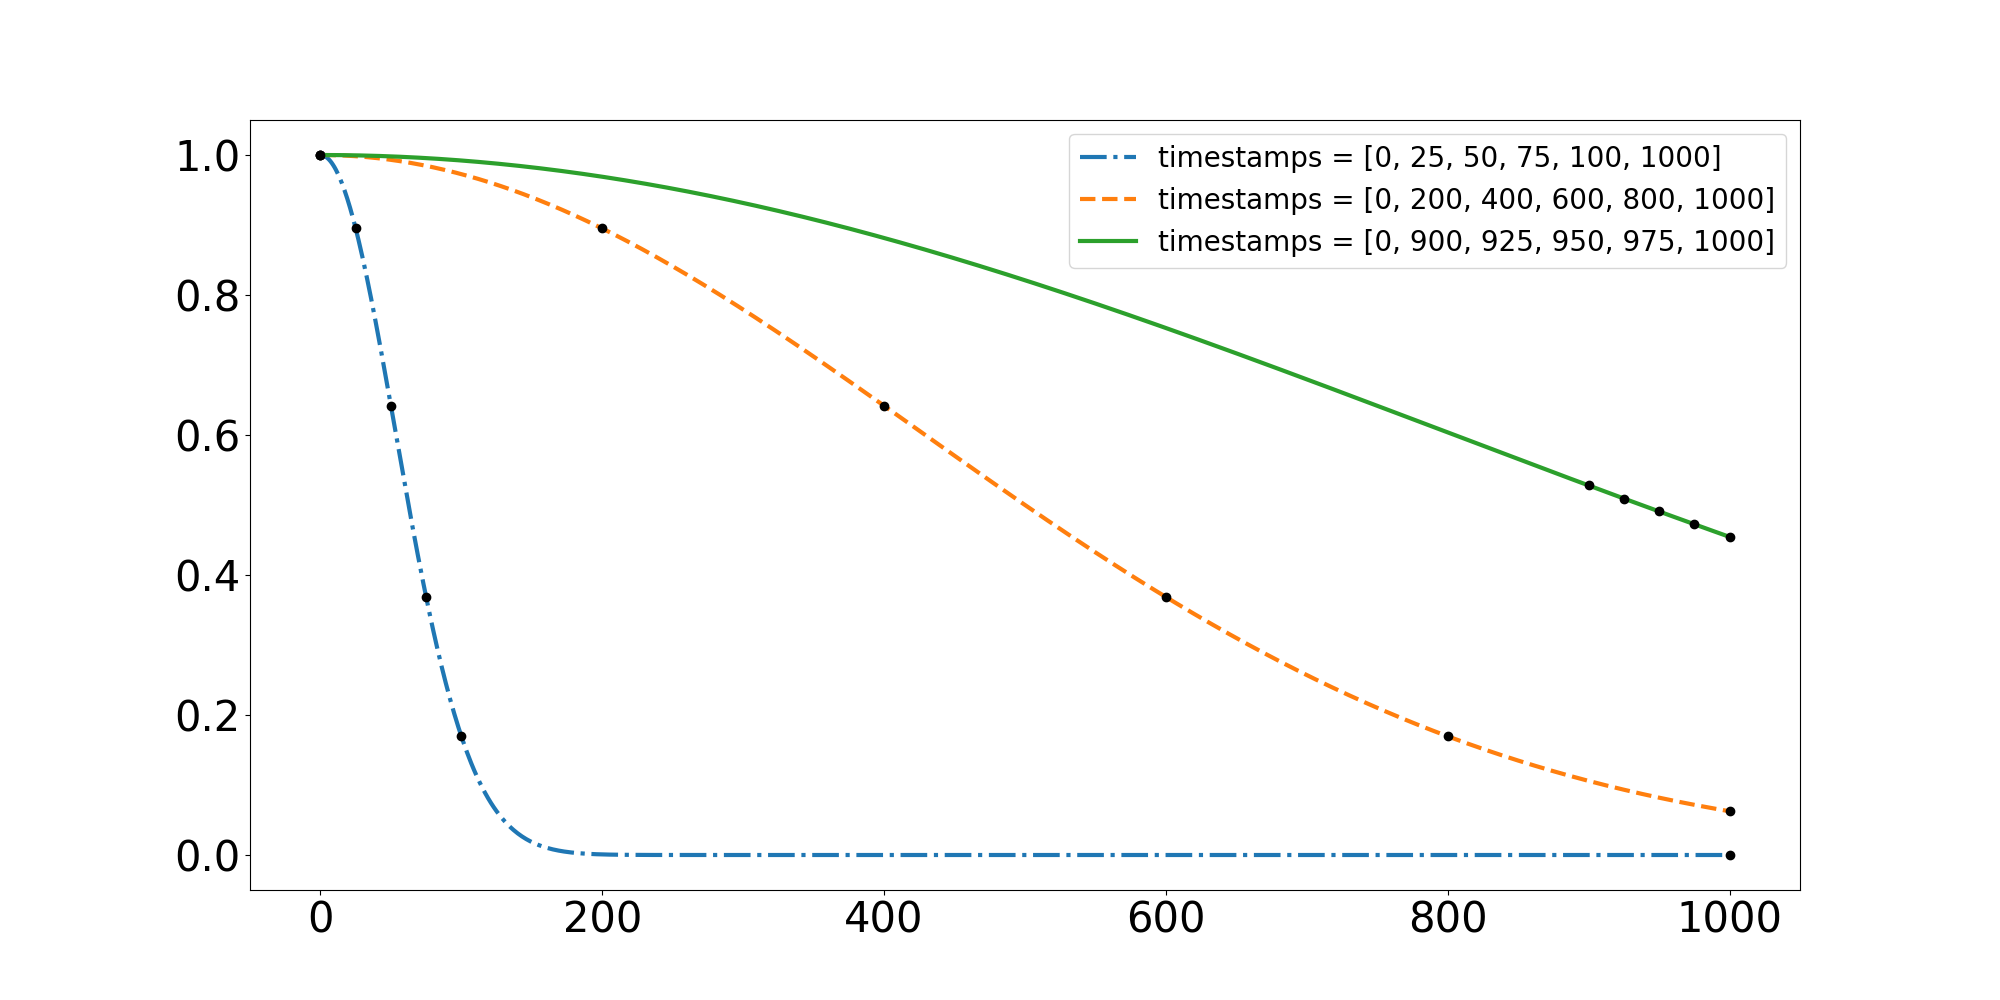
\includegraphics[width=\columnwidth]{weight-function-example.png}
	\caption{Weight functions for three timestamp vectors.}
	\label{fig:weight}
\end{figure}
For each transaction, we evaluate the vector of weights:

\[
w^{tx} = w_{k^{tx}_{opt}}(t^{tx})
\]

Let $X$ be the set of all transactions we consider.
Let $P$ be the set of IP addresses of nodes that appear in at least one of~$p$ vectors in $X$:

\[
P = \bigcup\limits_{tx \in X} p^{tx}
\]

We define an extended weight vector $v_{tx}$ for each~$tx$ by setting the weight of nodes in $P \backslash p^{tx}$ to zero and sorting the values in the weight vectors w.~r.~t.~the alphabetical order of~$P$.
We then calculate a matrix where an element in \mbox{$i$-th} row and~\mbox{$j$-th} column is the Pearson correlation of the extended weight vectors $v_{tx_i}$ and~$v_{tx_j}$.
This matrix can supposedly be transformed into a block-diagonal matrix with blocks (clusters) corresponding to transaction sources.
To reveal the clusters, we use spectral co-clustering~\cite{Dhillon2001} implemented in the Python \texttt{sklearn.cluster.bicluster} module~\cite{scikit-learn, scikitlearn2018}.
Given an input matrix $A$, the algorithm forms $A_n$ as follows:

\[
A_n = R^{-1/2}AC^{-1/2}
\]

$R$ is the diagonal matrix with entry $i$ equal to $\sum_{j} A_{ij}$, and~$C$ is the diagonal matrix with entry $j$ equal to $\sum_{i} A_{ij}$.
This defines the singular value decomposition (SVD) of the normalized matrix $A_n$.
The $l$ = $\lceil \log_2 k \rceil$ singular vectors $u_2,\dots,u_{l+1}$ and $v_2,\dots,v_{l+1}$ of $A_n$ may be used to solve a real approximation of the minimal cut problem.
Let $U$ be a matrix with columns $u_2,\dots,u_{l+1}$, and similarly for $V$ and $v_2,\dots,v_{l+1}$.
Then $Z$ is defined as:

\[
Z = 
\begin{bmatrix}
R^{-1/2} & U \\
C^{-1/2} & V
\end{bmatrix}
\]

The rows of~$Z$ are then clustered using the k-means algorithm to obtain the desired partitioning.


\subsection{Measuring clustering quality}

We use the Rand score as an external metric of clustering quality (see~\cite{Amigo2009}, Section~4.2).
A clustering algorithm decides for each pair of elements, whether to put it in the same cluster or different clusters.
Let $SS$,~$SD$,~$DS$, and~$DD$ be the numbers of transaction pairs defined as follows:
\begin{itemize}
	\item SS: same cluster, same category\footnote{Here we consider two categories: "our" and "foreign" transactions.} (our transactions in one cluster);
	\item SD: same cluster, different category (our and foreign transactions in one cluster);
	\item DS: different cluster, same category (our transactions in different clusters);
	\item DD: different cluster, different category (our and foreign transactions in different clusters).
\end{itemize}

The Rand score reflects the proportion of correct decisions:

\[
R = \frac{SS + DD}{SS + SD + DS + DD}
\]

Note that this assessment only considers clusters with "our" transactions, because we do not know whether any two "foreign" transactions should have been assigned to the same cluster.

We parameterize this metric with the minimal number of our transactions in a cluster required to consider this cluster in the calculation.
In our experiments, we only consider clusters with at least two of our transactions.
With no such threshold, large clusters with one of our transactions disproportionately increase $DD$ and bring the score close to $1$, which does not reflect the subjective amount of information an adversary acquires.


\subsection{Measuring the degree of deanonymization}

We measure the success of the attack using a quality score based on the \textit{anonymity degree}~\cite{Diaz2002}.
The goal is to assign to each transaction a probability that it originates from~$S_{control}$.
Initially, all transactions have equal probabilities.
The attacker adjusts the probabilities based on clustering results.
The anonymity degree measures the amount of information the attacker gains.

Let $p_i$ be the probability that a transaction~$i$ originates from~$S_{control}$.
$K$ is the total number of transactions.
The entropy is calculated as:

\[
H = -\sum_{i=1}^K p_i log_2(p_i)
\]

The maximum entropy is:

\[
H_{max} = log_2(K)
\]

The anonymity degree is defined as:

\[
d = \frac{H}{H_{max}}
\]

Our goal is to put transactions that originate from one target source $S_{control}$ into one cluster.
Out of~$K$~captured transactions, $k$ are issued from~$S_{control}$.
For each transaction~$i$, the a priori probability of it having originated from~$S_{control}$ is $p_i = k / K$.

We then divide all transactions into clusters.
However, multiple clusters may correspond to~$S_{control}$.
To account for this, each cluster is assigned a \textit{weight} that reflects how likely this cluster represents $S_{control}$.
Consider an example.
The attacker captures $10$~transactions $t_0, \dots, t_9$.
Five of them, $t_0, \dots, t_4$, originate from the target source~$S_{control}$.
The clustering algorithm yields three clusters: $c_a = \{t_0, t_1, t_2, t_3\}, c_b = \{t_4, t_5, t_6, t_7\}, c_c = \{t_8, t_9\}$.
The attacker knows that $t_0$ and~$t_4$ originate from~$S_{control}$ and assigns a weight of~$0.5$ to clusters $c_a$ and~$c_b$, and a weight of~$0$ to cluster~$c_c$.
Therefore, the total "probability weight" of transactions from $S_{control}$ is distributed evenly among $c_a$ and~$c_b$ ($t_0, \dots, t_7$).
Note that the true distribution is $1$ for transactions $t_0, \dots, t_4$ and~$0$ for all others.

Finally, we calculate the \textit{adjusted} anonymity degree accounting for cluster weights.
We calculate the median square error~$e$ between the vectors of probabilities $p_i$ derived by the attacker and the actual probabilities.
The adjusted anonymity degree is defined as follows:

\[
d_{adj} = 1 - (1 - e) \times (1 - d)
\]

Consider two edge case examples.
If $e = 0$ (the attacker correctly guessed the~$S_{control}$ cluster), $d_{adj} = d$.
If $e = 1$ (the attacker's cluster weights do not at all reflect the reality), $d_{adj} = 1$ (the system retains full anonymity).


\section{Implementation details}

We use a modified Bitcoin network probing tool \texttt{bcclient}~\cite{Pustogarov2017} to maintain parallel connections to peers and log incoming messages.
Multiple parallel connections increase our chance to be among the first peers to learn about a new transaction despite broadcast randomization.
The tool is relatively easy to adapt for usage with Dash and Zcash, which mostly inherit the networking layer from Bitcoin Core.
We re-compile \texttt{bcclient} with modified constants (port numbers, protocol magic bytes, DNS seeder addresses).
For Monero, which is not based on the Bitcoin~Core codebase, we modify the reference implementation (\texttt{monerod}).
We add the required logging and disable the built-in limits on the total bandwidth and artificial delays between network requests.

First, we collect a fresh snapshot of the network.
We start by resolving the bootstrapping DNS seeds.
We try to connect to all known peers and ask them for peers they know using \texttt{getaddr} command.
We recursively repeat the process three times.

For each transaction announcement, we log the transaction hash, the IP that has announced it, and the timestamp of this event.
We only log \texttt{inv} messages, and never continue with the \texttt{getdata} -- \texttt{tx} exchange.
For selected experiments on the Bitcoin testnet, we also log \texttt{addr} messages.
Address announcements allow us to infer the set of most probable IP addresses that correspond to each transaction cluster.

We use additional Python scripts to issue series of transactions from two different nodes.
For each transaction set (learning set and control set) for each experiment, we emit a series of transactions to our own newly generated addresses.
We use the command line interface of the underlying full node (such as \texttt{bitcoind} for Bitcoin).
To send a transaction, we use \texttt{sendtoaddress} command.
We generate a new address for each transaction with \texttt{getnewaddress}.
The payment amounts are generated uniformly at random from an interval between the minimum and the maximum allowed amount.
The maximum amount is $10$~times higher than the minimum amount.
The minimum amounts for Bitcoin and Zcash are $0.00001$~BTC and $0.0005$~ZEC, respectively.

Experiments on the cryptocurrencies based on the Bitcoin~Core codebase are implemented similarly.
For Zcash, we issue both transactions that involve shielded addresses (we call such transactions shielded for short) and transactions between transparent addresses (i.e.,~transparent transactions).
Issuing transparent transactions is similar to issuing transactions in Bitcoin.
For shielded transactions, we use \texttt{z_getnewaddress} to generate a new address and \texttt{z_sendmany} to send a transaction.

We use Python scripts to process the log.
We parse the log, extract the relevant information (transaction hashed and timestamps), and save the data in a more compact JSON format.
We then analyze the data, perform the clustering, and visualize the results.

The number of transactions we issue per experiment is limited due to the behavior of Bitcoin~Core when spending unconfirmed UTXOs.
It does not allow creating chains of unconfirmed transactions of length~$25$~or more.
Therefore, issuing more transactions within a short time frame (shorter than the block generation interval) demands creating multiple confirmed UTXOs in advance at both issuing nodes, which would require additional time and effort during the setup phase of each experiment.
Splitting the transactions in multiple chains and increasing the length of the experiment would lead to difficulties in parsing and processing the logs.


\section{Experimental evaluation}

The outline of our experiment is as follows:

\begin{enumerate}
	\item collect a fresh list of live peers;
	\item establish multiple parallel connections to them;
	\item launch the listening nodes and start logging \texttt{inv} and \texttt{addr} messages;
	\item launch two nodes $S_{learn}$ and~$S_{control}$;%, so that their initial \texttt{addr} advertisements are logged;
	\item issue two series of transactions: the learning set from~$S_{learn}$ and the control set from~$S_{control}$;
	\item for each considered number $N$ of first propagations, calculate the transaction correlation matrix;
	\item run the clustering algorithm with various assumed average numbers of transactions per cluster;
	\item choose the best clustering by Rand score based on the "learning" set;
	\item in the best clustering, assign the cluster weights proportionally to the distribution of known transactions from~$S_{control}$;
	\item assign zero probability of being in~$S_{control}$ to transactions from~$S_{learn}$;
	\item re-distribute the probability weight among transactions in each cluster;
	\item calculate the final adjusted anonymity score;
	\item re-arrange the clusters such that high correlation values are close to the main diagonal;
	\item visualize the results.
\end{enumerate}

We visualize the results with heatmaps.
We assign a color to each element of the correlation matrix.
A darker color at the intersection of the~\mbox{$i$-th} row and~\mbox{$j$-th} column represents a stronger correlation of weight vectors of~\mbox{$i$-th} and~\mbox{$j$-th} transactions.
The heatmap is diagonally symmetric by definition: each vector is perfectly correlated with itself.
We permute rows and columns such that the highly correlated elements are close to the main diagonal.
We expect such permutation to reveal the block-diagonal structure of the matrix.


\subsection{Results for desktop wallets}

We evaluate our method by clustering our own transactions in Bitcoin (testnet and mainnet) and Zcash.
For these experiments, we log the traffic for $15$~minutes.
For Dash and Monero, we run the clustering algorithm without calculating the anonymity degree.
We obtain clearly visible clusters, which indicates that our approach is applicable to these cryptocurrencies as well.
In the experiments on the Bitcoin mainnet, we deliberately do not attempt to occupy all connection slots and operate only on a subset of~$1\,000$~nodes (out of approximately $10\,000$~nodes reachable at any given time~\cite{Bitnodes}).
In this section, we refer to the node that logs the incoming messages as the \textit{listener}.
Following the terminology of~\cite{Biryukov2014}, \textit{servers} are peers that accept incoming connections.

% California: experiment-1541509693
% Tokyo: experiment-1541511845
% Frankfurt: experiment-1541513977
% 3-experiment: experiment-1541516997
\begin{table*}[!t]
	\normalsize
	\caption{Experimental results of transaction clustering for Bitcoin testnet and Zcash.}
	\centering
	\begin{tabular}{|l|l|c|c|c|c|c|}
		\hline
		Network & Listener & Anon\@. deg. & Servers & Avg free slots & Tx \texttt{inv}s & \texttt{addr}s \\
		\hline
		Bitcoin test & California & $0.83$ & $1\,141$ & $64$ & $139$ & $402$ \\
		Bitcoin test & Tokyo & $0.80$ & $1\,128$ & $64$ & $193$ & $414$ \\
		Bitcoin test & Frankfurt & $0.72$ & $1\,137$ & $64$ & $172$ & $403$ \\
		Bitcoin test & combined & $0.63$ & $1\,154$ & $63$ & $250$ & $1\,321$ \\
		Bitcoin main & Frankfurt & $0.88$ & $1\,000$* & $25$* & $3\,238$ & $11\,300$ \\
		Zcash & Frankfurt & $0.86$ & $206$ & $36$ & $62$ & $1\,086$ \\
		\hline
	\end{tabular}
	\label{tab:results}
\end{table*}

\subsubsection{Bitcoin testnet}

We perform four experiments on the Bitcoin testnet using listeners in different geographical locations: Frankfurt (Germany), Tokyo (Japan), and North California (the US).
We conduct three experiments with each of the listeners and the fourth experiment using all listeners simultaneously.
To use multiple listeners in one experiment, we distribute live peers equally among the three listeners.
Each listener connects only to the peers from its chunk of the list.
We then merge the log files.
The fourth experiment measures the advantage an adversary gains from using geographically distributed listeners.
Each listener attempts to establish $117$~connections to each assigned peer.

In each experiment, we issue two sets of test transactions (the learning and the control sets) containing $30$~transactions each from computers located in Luxembourg.
We denote $10$~transactions from the control set as "known" to estimate the anonymity degree.

The number of live peers collected by each of the listeners is close, which indicates that we obtain a complete view of the network.
The number of received transactions varies little between experiments, whereas the number of \texttt{addr} messages is significantly higher in the multi-listener experiment: \texttt{addr} messages propagate through the network more slowly than transactions.
The average number of available connection slots is independent of the location of the listener.

The anonymity degree calculated on our own transactions indicates a substantial loss of privacy (Table~\ref{tab:results}).
The "*"~sign in the table indicates the experiments where we only connected to a subset of available nodes.
The joint experiment with three geographically distributed listeners gained the best results with an anonymity degree of~$0.63$.
Out of the three single-listener experiments, only the Frankfurt experiment shows a lower anonymity degree.
We explain it by a small geographical distance between the listener and the transaction source.
The results are presented in Figures~\ref{fig:bitcoin-testnet-california},~\ref{fig:bitcoin-testnet-tokyo},~\ref{fig:bitcoin-testnet-frankfurt}, and~\ref{fig:bitcoin-testnet-combined} (ticks along the axes denote our transaction from the control set).


\begin{figure*}
	\centering
	\begin{minipage}{0.5\textwidth}
		\centering
		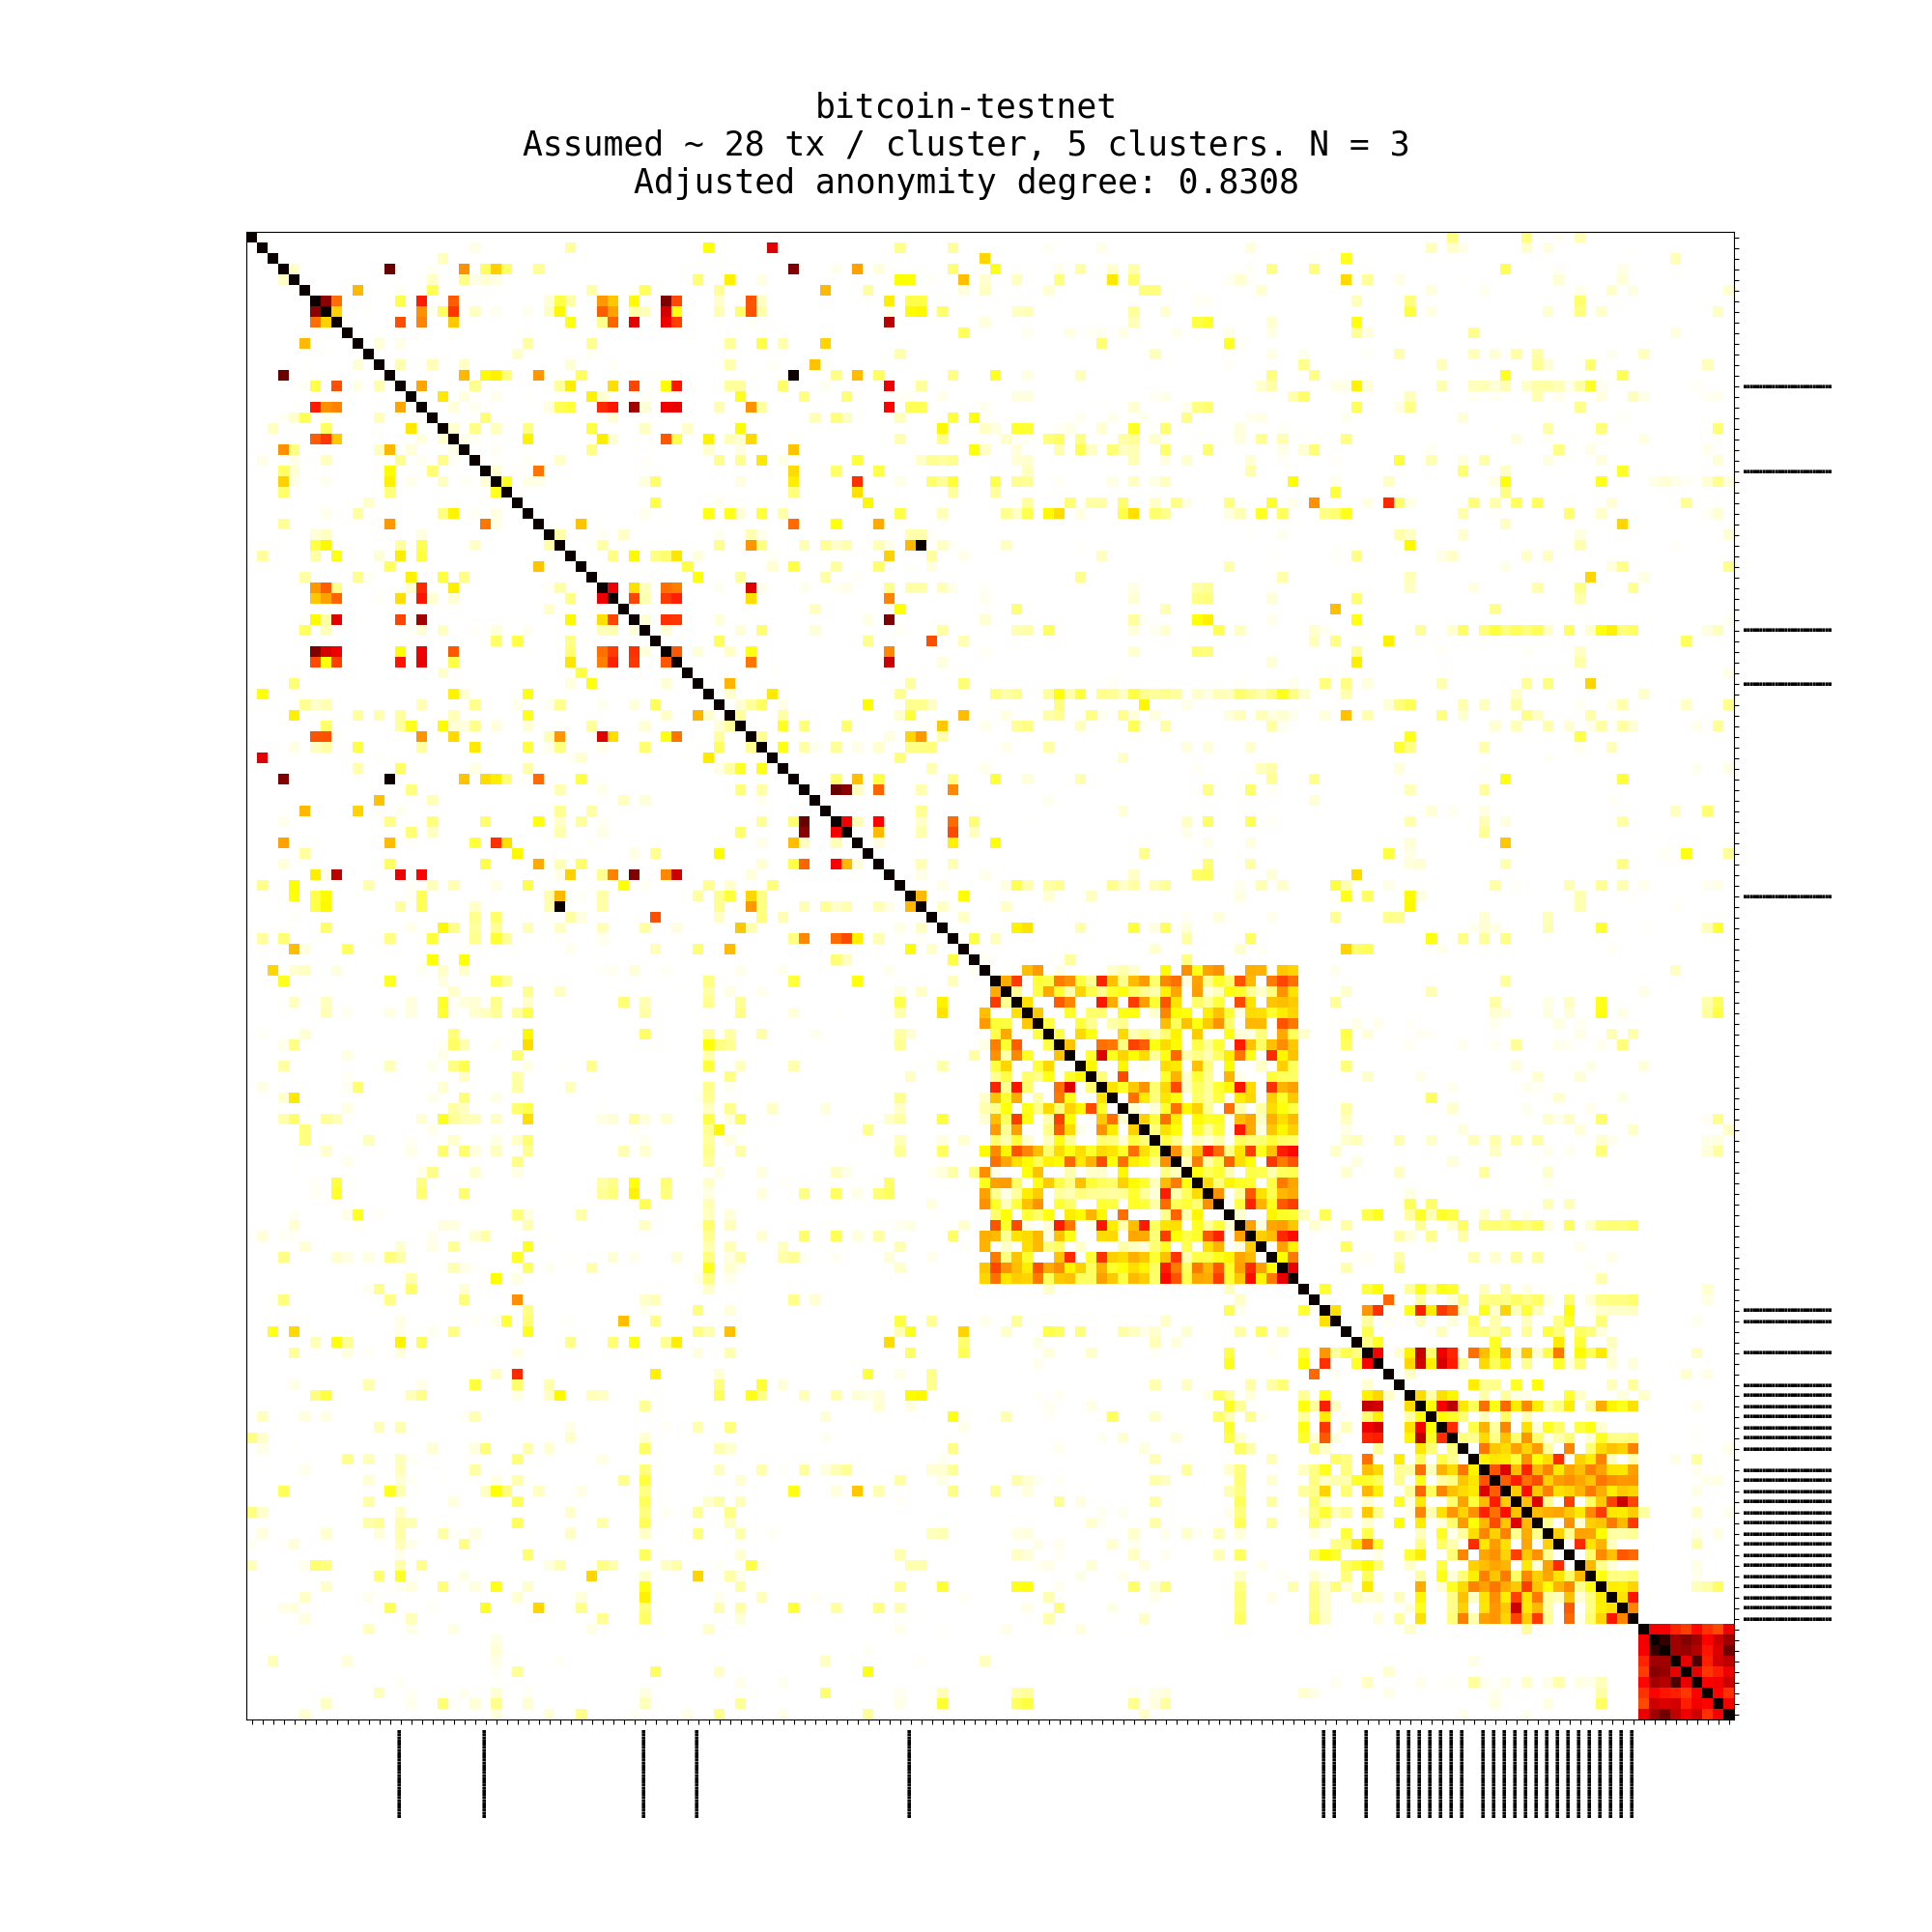
\includegraphics[width=\columnwidth]{bitcoin-testnet-1541509693-California.png}
		\caption{Transaction clustering for Bitcoin testnet (listener in California).}
		\label{fig:bitcoin-testnet-california}
	\end{minipage}\hfill
	\begin{minipage}{0.5\textwidth}
		\centering
		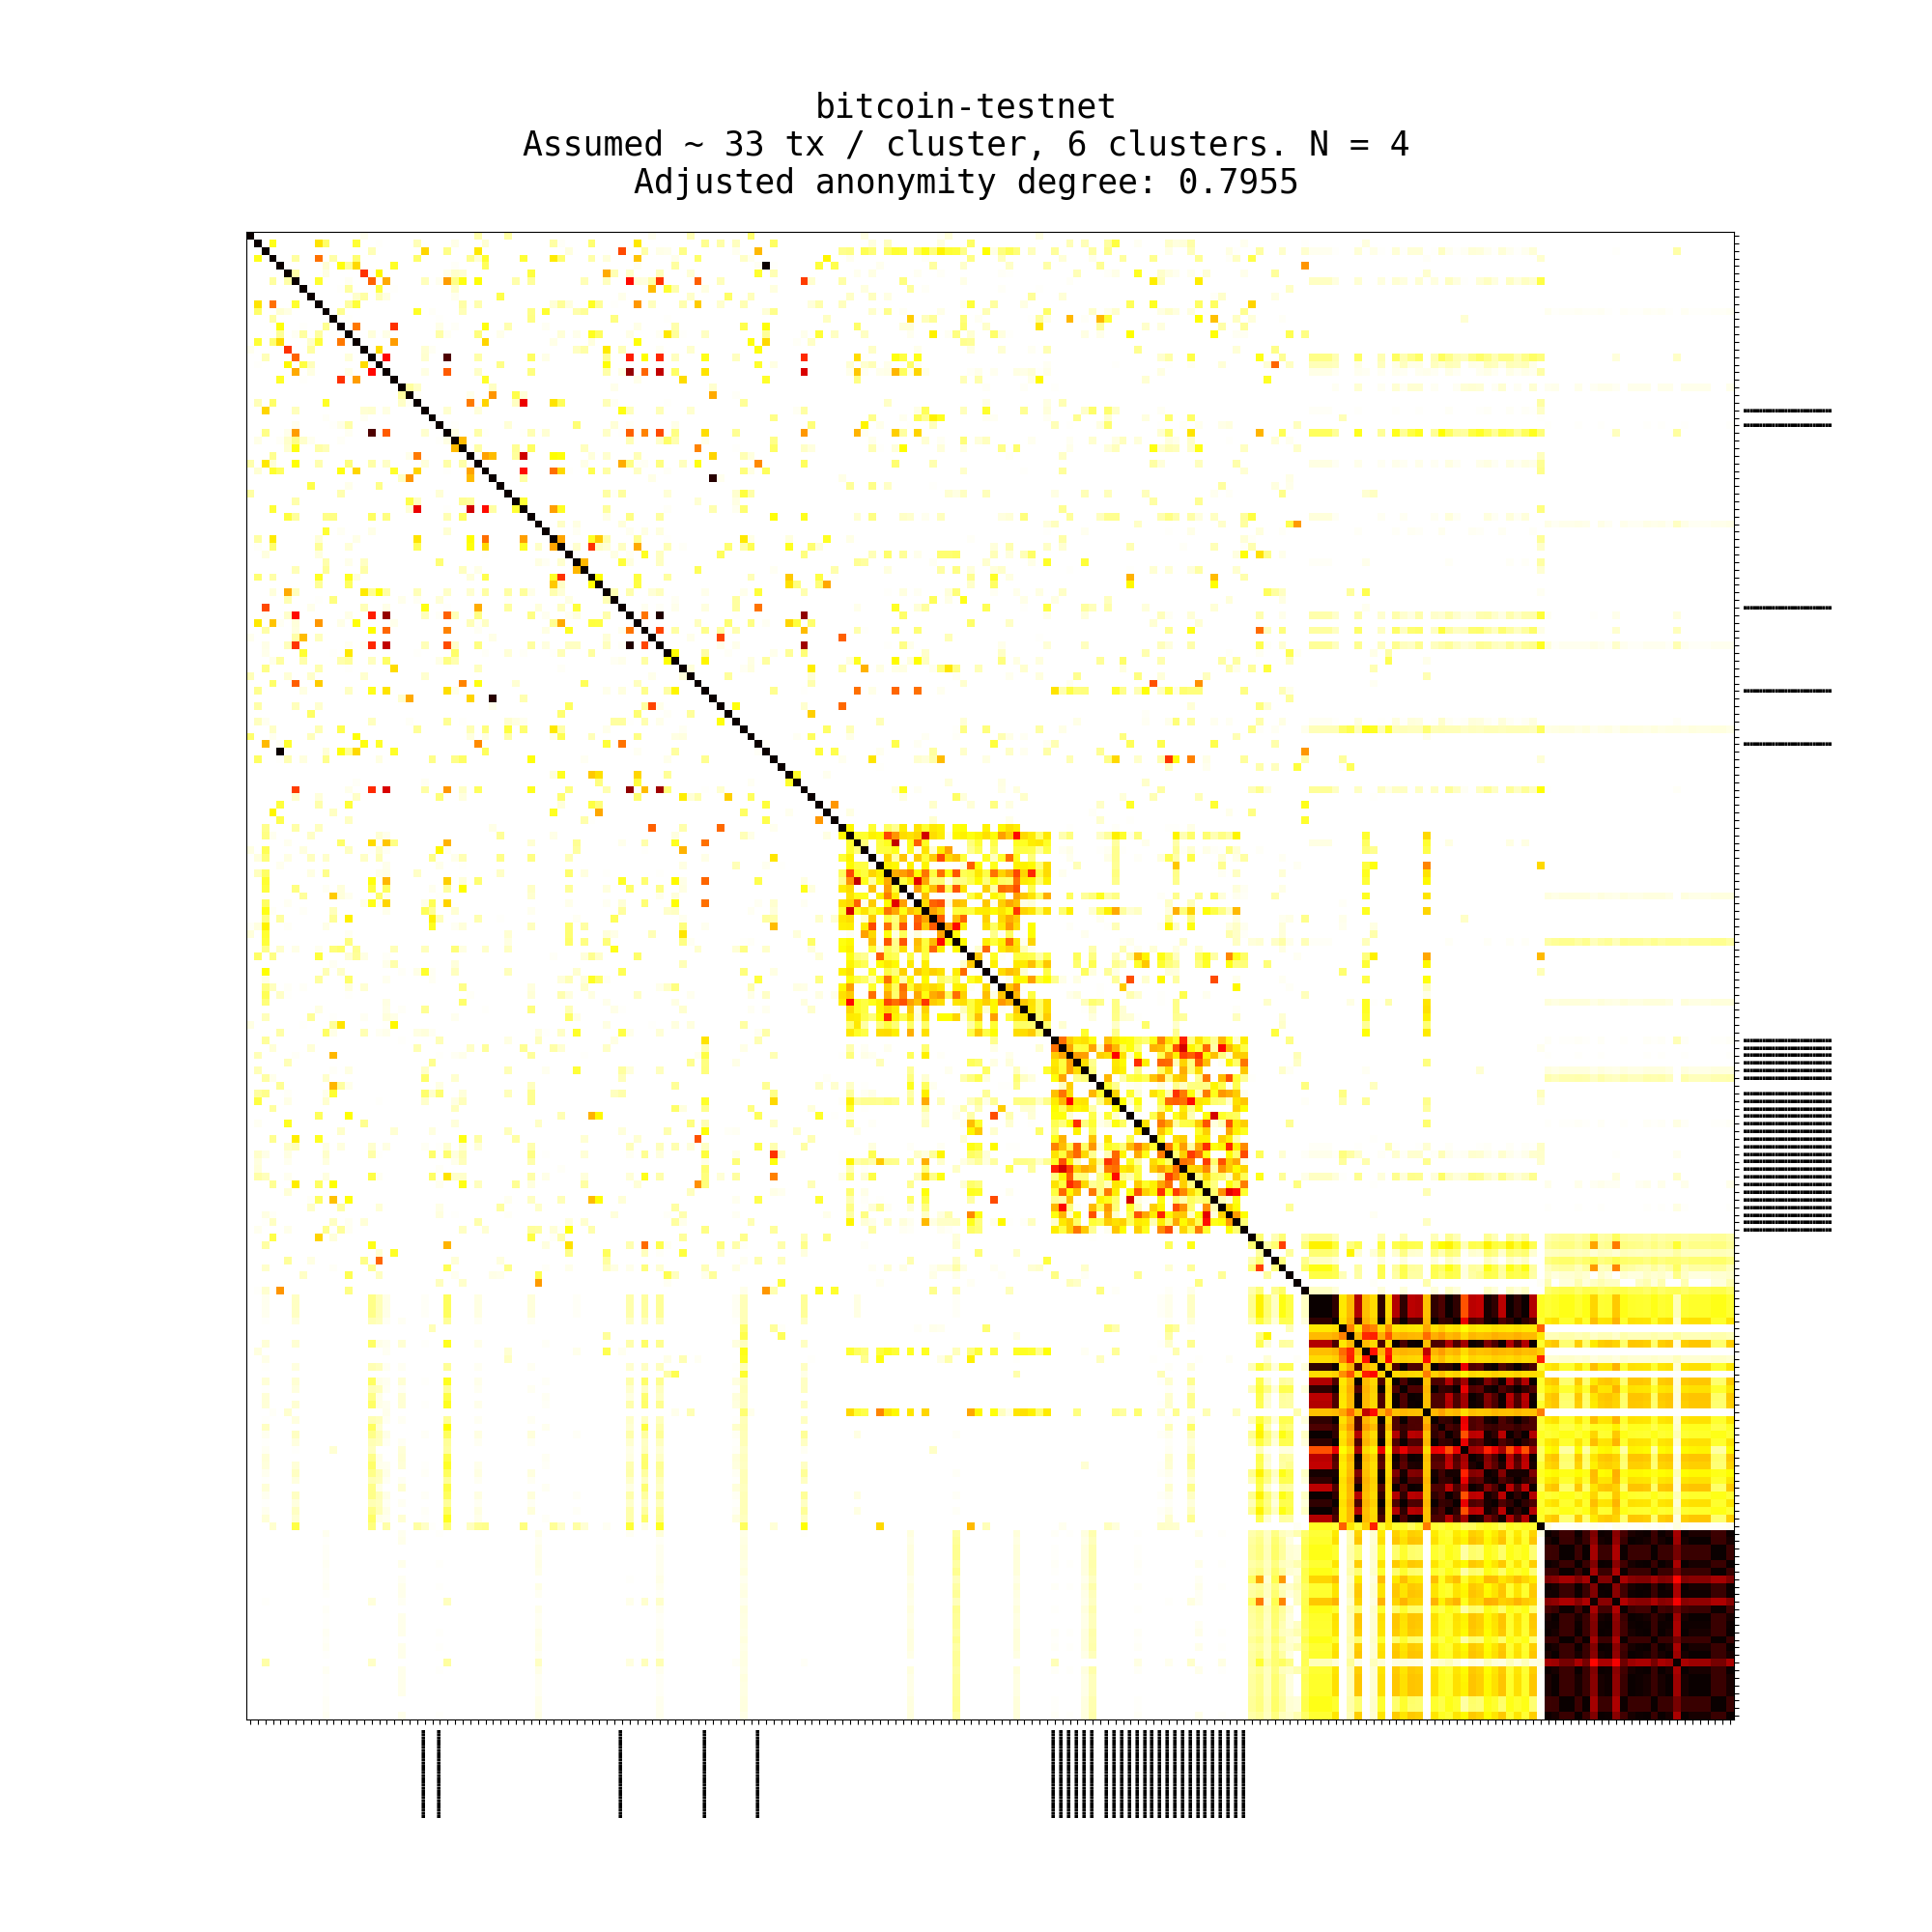
\includegraphics[width=\columnwidth]{bitcoin-testnet-1541511845-Tokyo.png}
		\caption{Transaction clustering for Bitcoin testnet (listener in Tokyo).}
		\label{fig:bitcoin-testnet-tokyo}
	\end{minipage}\hfill
\end{figure*}

\begin{figure*}
	\centering
	\begin{minipage}{0.5\textwidth}
		\centering
		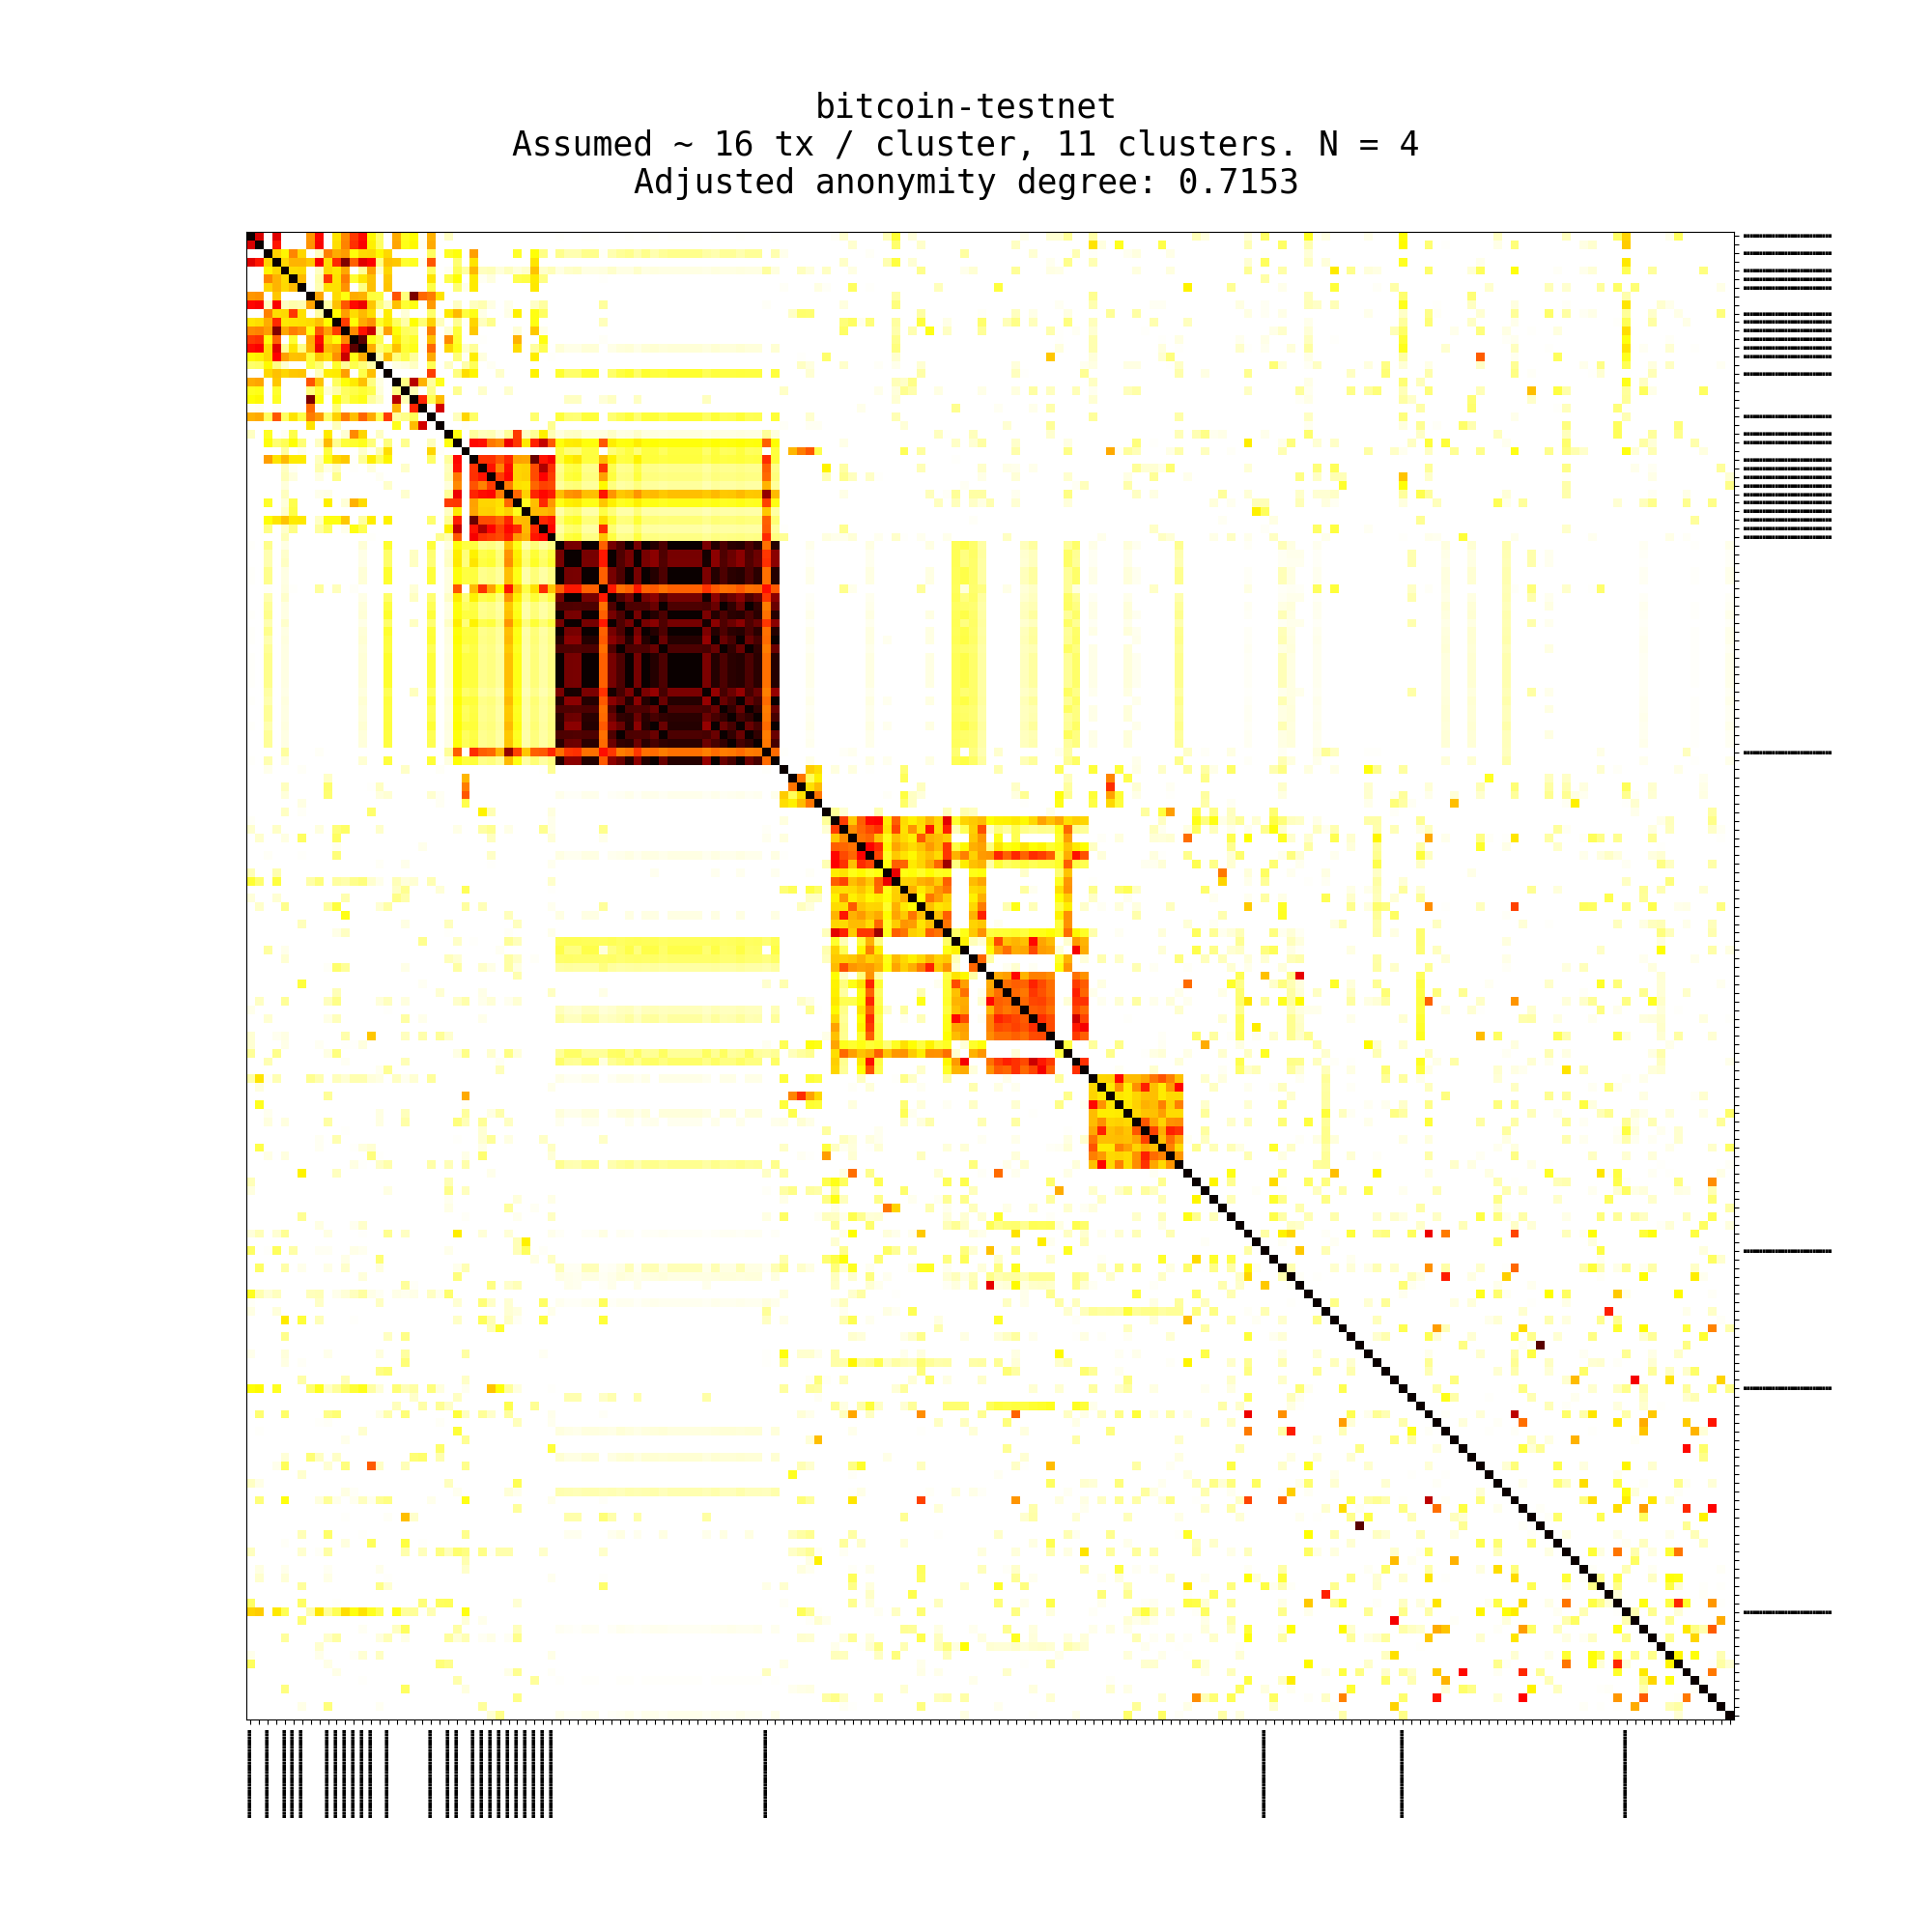
\includegraphics[width=\columnwidth]{bitcoin-testnet-1541513977-Frankfurt.png}
		\caption{Transaction clustering for Bitcoin testnet (listener in Frankfurt).}
		\label{fig:bitcoin-testnet-frankfurt}
	\end{minipage}\hfill
	\begin{minipage}{0.5\textwidth}
		\centering
		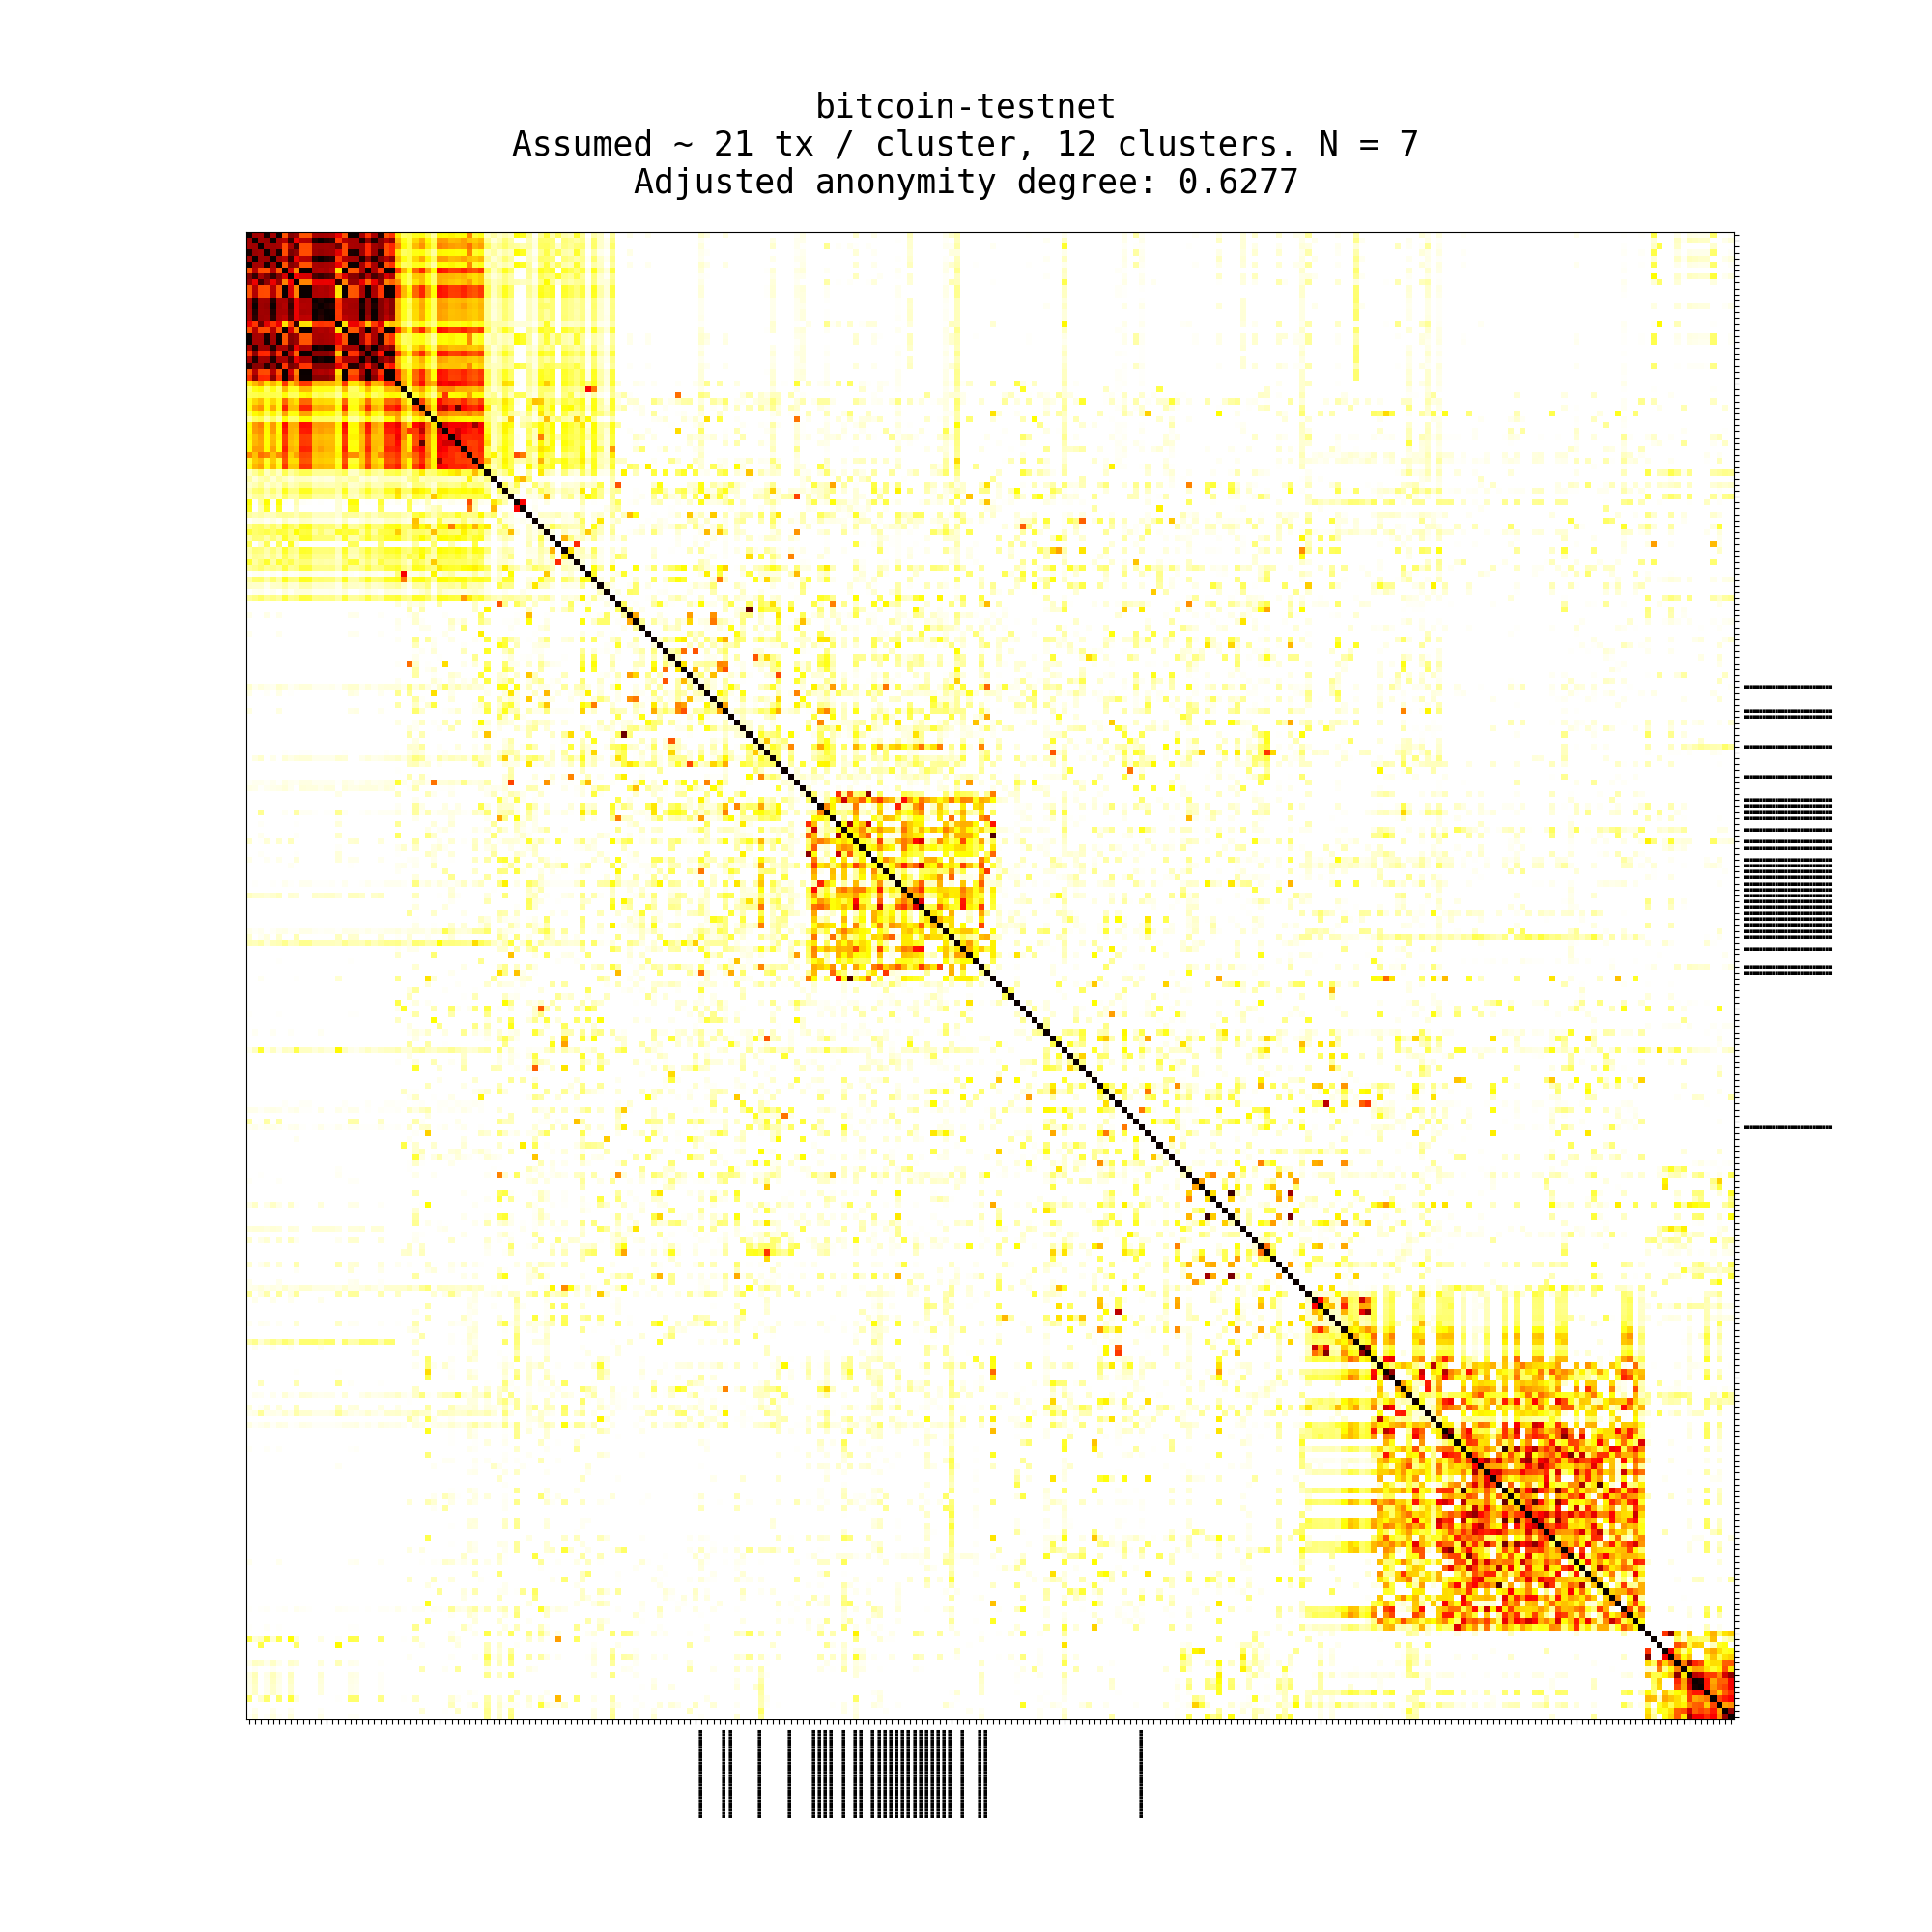
\includegraphics[width=\columnwidth]{bitcoin-testnet-1541516997-combined.png}
		\caption{Transaction clustering for Bitcoin testnet (combined listeners).}
		\label{fig:bitcoin-testnet-combined}
	\end{minipage}\hfill
\end{figure*}


\paragraph{Estimating the original IP}

We use the \texttt{addr} messages to determine (with some level of precision) the IP address of the transaction source.
In our experiments, we first launch the listener and only then launch the issuing nodes.
This allows the listener to capture the \texttt{addr} messages issued by the issuing nodes during bootstrapping.
Address messages propagate through the network more slowly than transactions and are periodically re-broadcast.
A listener can distinguish between \texttt{addr} messages of recently joined nodes and re-broadcasts of older \texttt{addr} messages.
If only one or two nodes announce an IP address, we assume it is a re-broadcast.
If more nodes announce an IP address, we assume that the node has just joined the network or is re-advertising its IP address.

We leverage the \texttt{addr} messages as follows.
For each cluster, we determine the IPs of the most "important" nodes, i.e.,~nodes we assume might be the source or its entry nodes.
For each transaction in the cluster, we sum up the weights of all IPs that have relayed it to us.
We assume the top $10\%$~of most weighted IPs to be the entry nodes.
The intuition is that the entry nodes are among the first to relay \texttt{addr} messages from the source.
Therefore, we assume that an \texttt{addr} message relayed by a set of IPs that substantially intersects with the entry nodes contains the IP address of the source of the cluster.

We apply this heuristic to the Bitcoin testnet experiments.
We consider the clusters that mostly consist of control transactions.
In three out of four experiments, the actual IP address is among the top five most "important" IPs.
This result indicates that an adversary can narrow down the search for the source IP address to only a handful of IPs.

\subsubsection{Bitcoin mainnet}

We perform one experiment on the Bitcoin mainnet with a listener located in Frankfurt.
The learning and control sets consist of~$20$~transactions each.
Five transactions from the control set are assumed "known" for anonymity degree calculation.

The results are presented in Table~\ref{tab:results} and Figures~\ref{fig:bitcoin-mainnet} and~\ref{fig:zcash}.
The correlation matrix also exhibits the "clustering" behavior, though the anonymity loss is smaller than for the Bitcoin testnet and Zcash.
We explain these weaker results by multiple factors.
First, the Bitcoin mainnet is substantially larger than other networks that we consider.
More transactions in Bitcoin constitute a larger anonymity set.
Second, Bitcoin nodes provide fewer connection slots and often limit the number of slots one IP can occupy.
A low number of parallel connections decreases the probability that our listener learns about a new transaction quickly.
Third, we only establish up to $50$~connections to $1\,000$~peers to avoid disrupting the network, and due to resource constraints.

\begin{figure*}
	\centering
	\begin{minipage}{0.5\textwidth}
		\centering
		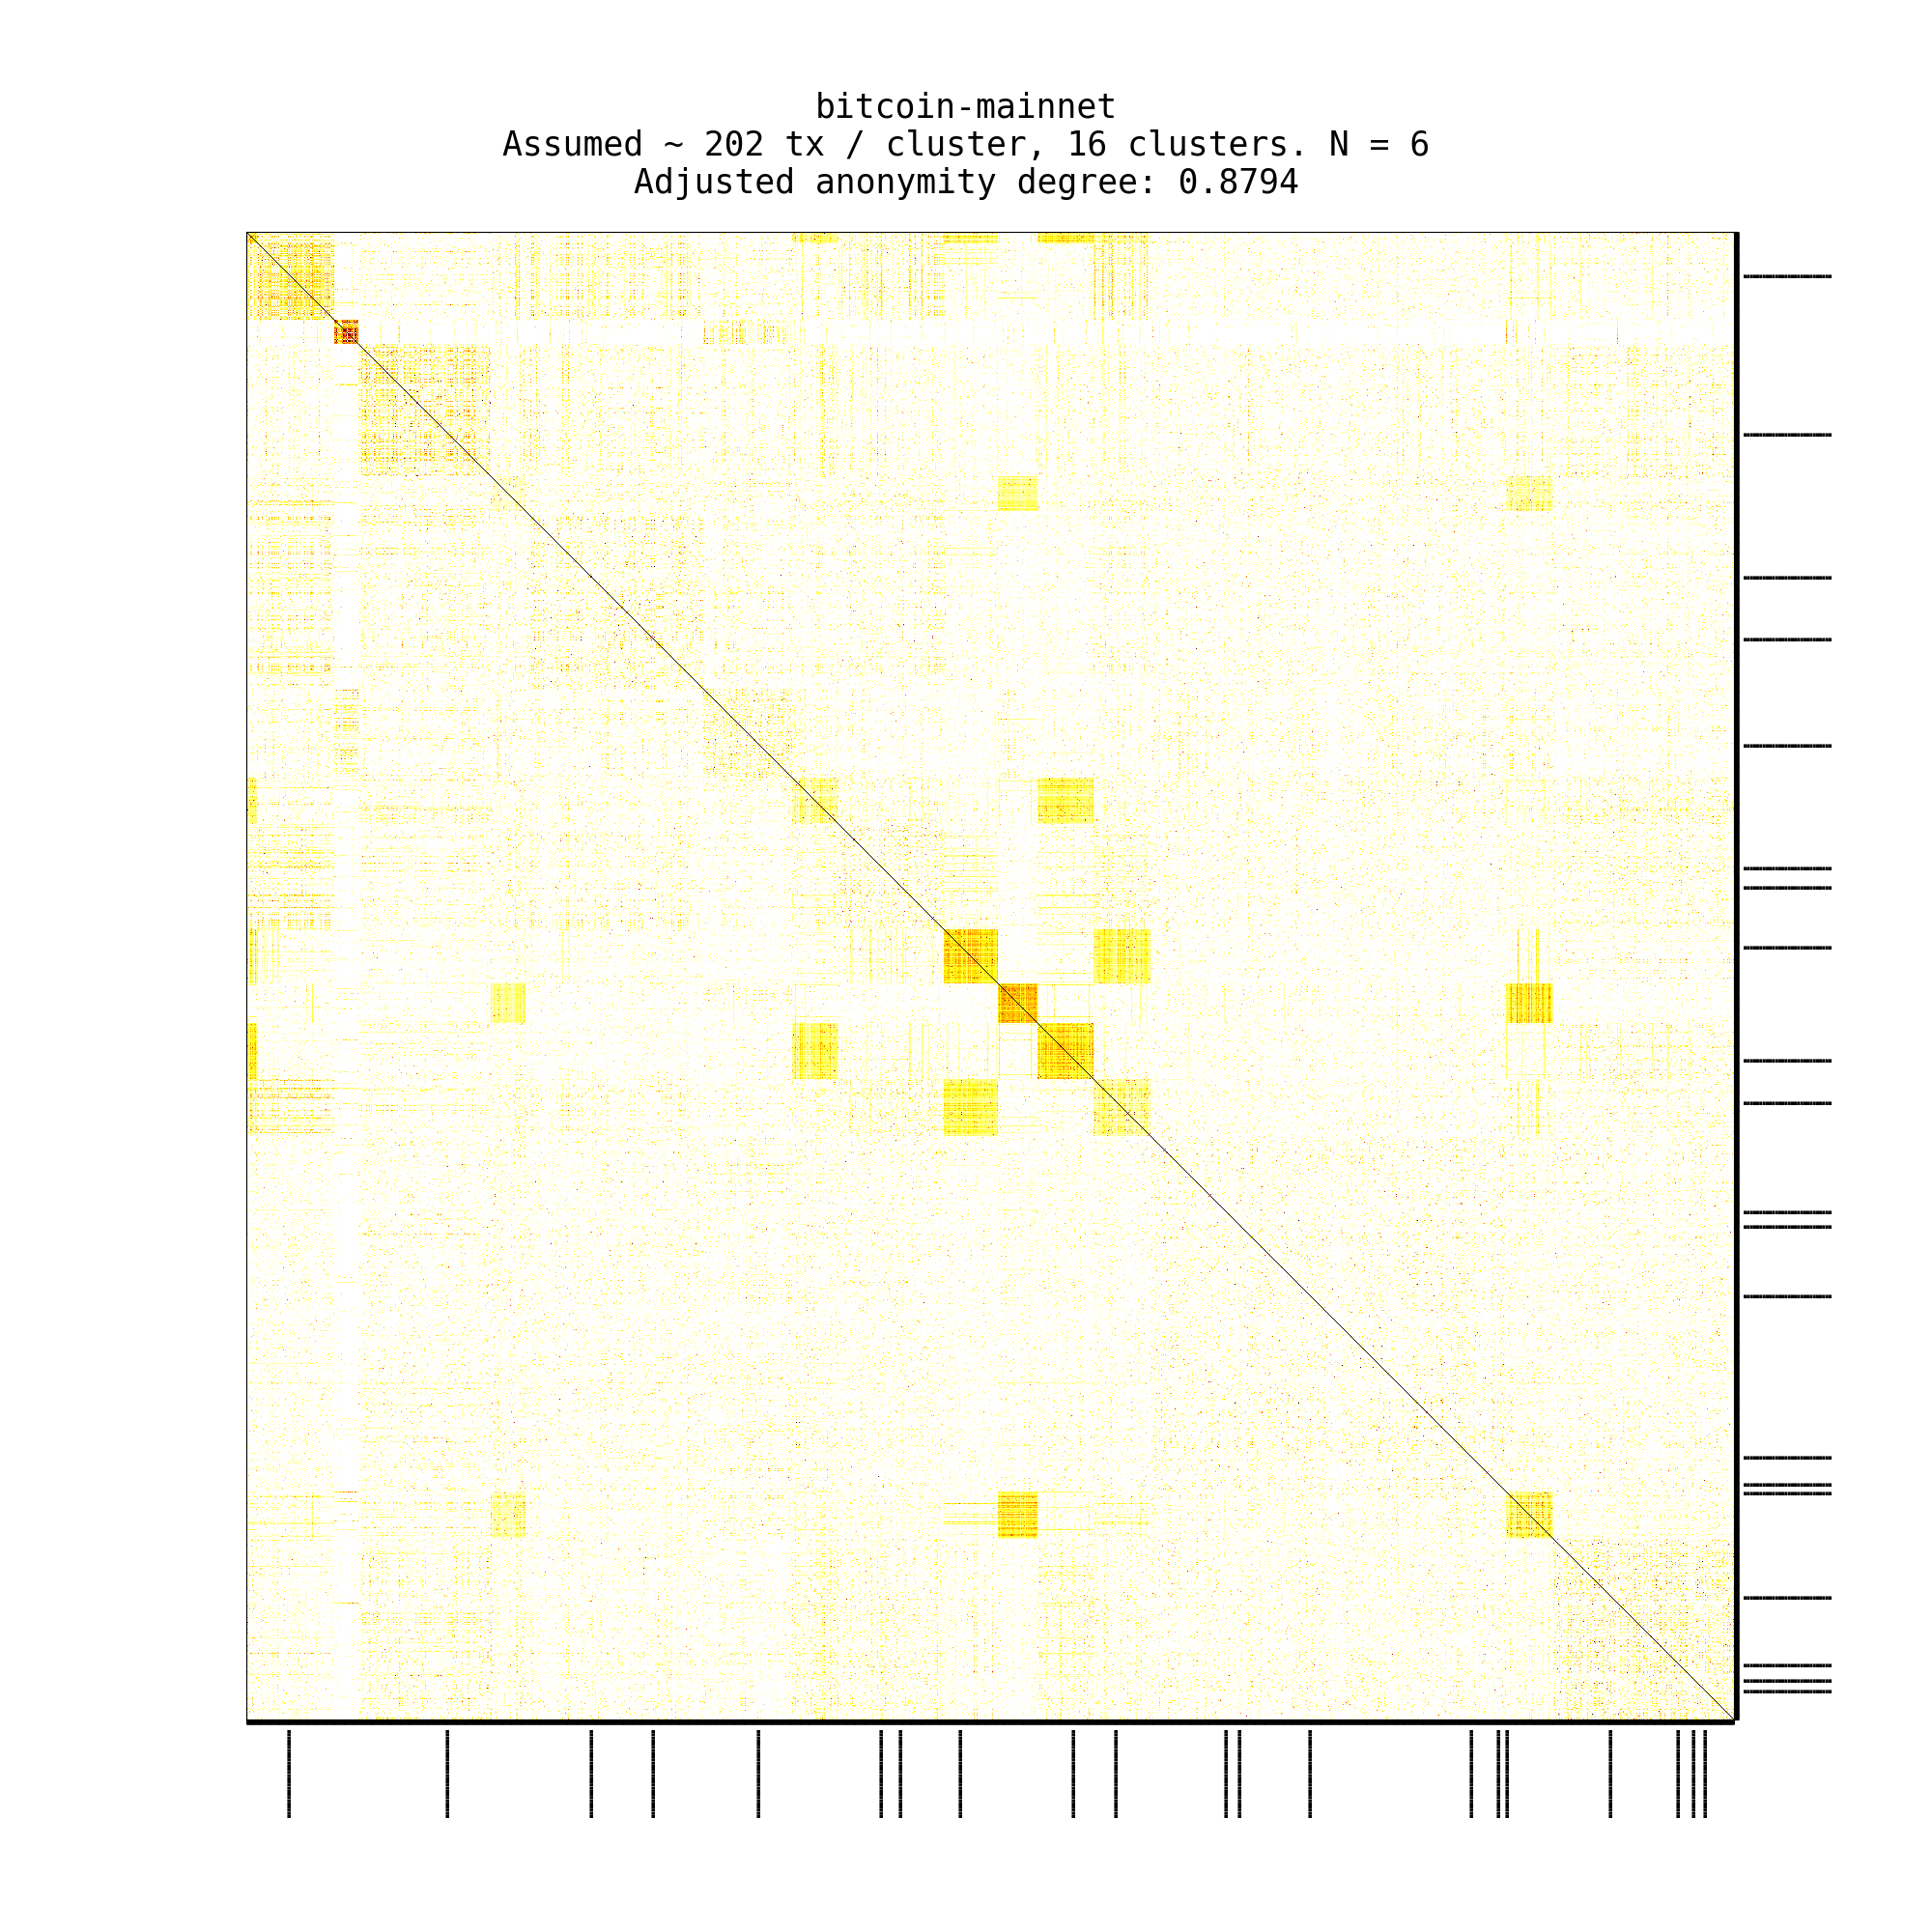
\includegraphics[width=\columnwidth]{bitcoin-mainnet-1542054034-fig-correlations-202-txcl-006-N-Rand-best.png}
		\caption{Transaction clustering for Bitcoin mainnet.}
		\label{fig:bitcoin-mainnet}
	\end{minipage}\hfill
	\begin{minipage}{0.5\textwidth}
		\centering
		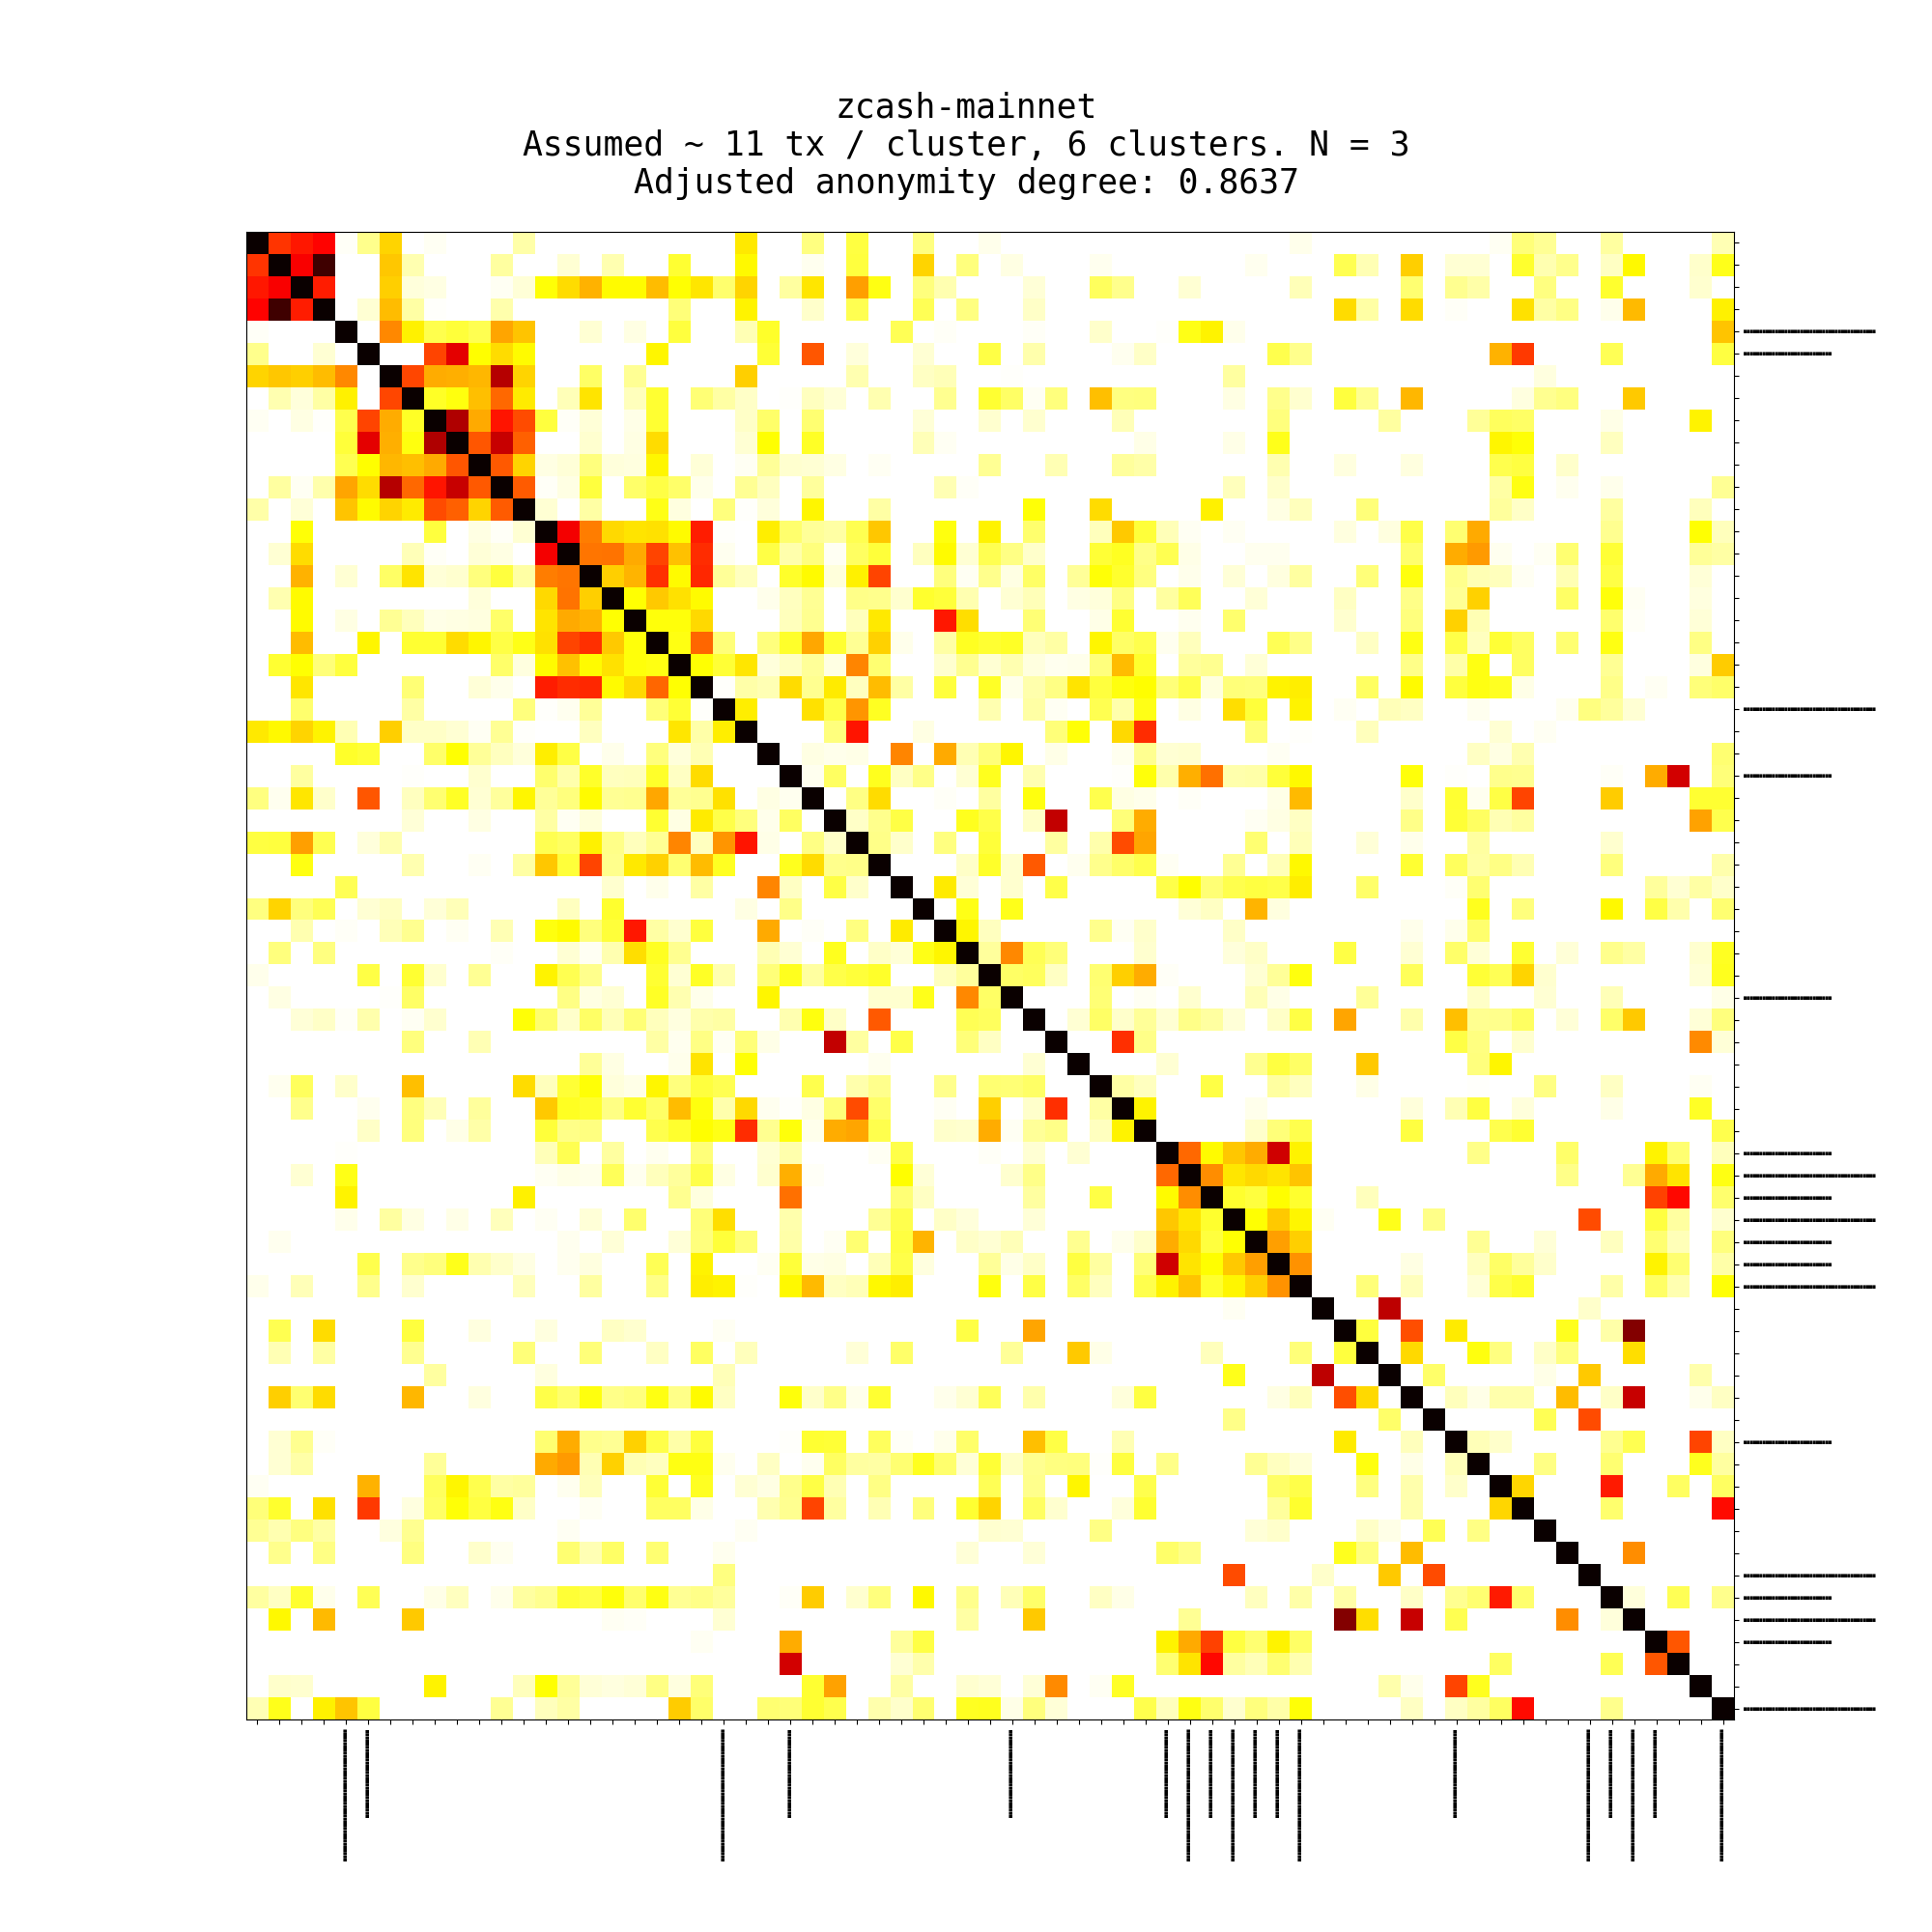
\includegraphics[width=\columnwidth]{zcash-mainnet-1541938472-Frankfurt.png}
		\caption{Transaction clustering for Zcash.}
		\label{fig:zcash}
	\end{minipage}\hfill
\end{figure*}

\subsubsection{Zcash}

Zcash is based on the Bitcoin~Core codebase.\footnote{Bitcoin~Core~version~0.11.2 (commit~7e27892), November~2015.}
As of the time of our experiments (mid-2018), Zcash uses trickling for broadcast randomization, while Bitcoin uses diffusion.
Zcash does not provide privacy by default: zero-knowledge proofs are used only in transactions involving \textit{shielded} addresses~\cite{Kappos2018}.
Most transactions happen between \textit{transparent} addresses and have no added privacy-preserving mechanisms compared to Bitcoin.

We perform one experiment on the Zcash mainnet with a listener located in Frankfurt.
The learning and control sets consist of~$20$ and~$18$~transactions, respectively.
Eight~out of~$18$~control transactions use shielded addresses (transactions from a t-address to a z-address, also known as t-to-z).
We use $6$~control transactions as "known" for anonymity degree estimation.

The results are presented in Figures~\ref{fig:bitcoin-mainnet} and~\ref{fig:zcash}.
T-to-z transactions from the control set are marked with longer ticks.
Note that our method clusters transactions involving both transparent and shielded addresses.

We notice that Zcash peers offer far fewer connection slots on average: $36$~compared to $64$~on the Bitcoin testnet (Figures~\ref{fig:free-slots-bitcoin} and~\ref{fig:free-slots-zcash}).
Many servers only accept fewer than ten connections.
These results may reflect a larger share of \textit{protected} nodes in Zcash.
Protected nodes use firewalls or other network-level mechanisms to limit the number of connections from each IP\@.
However, an adversary can overcome this limitation by purchasing IP addresses from a cloud provider.

\begin{figure*}
	\centering
	\begin{minipage}{0.5\textwidth}
		\centering
		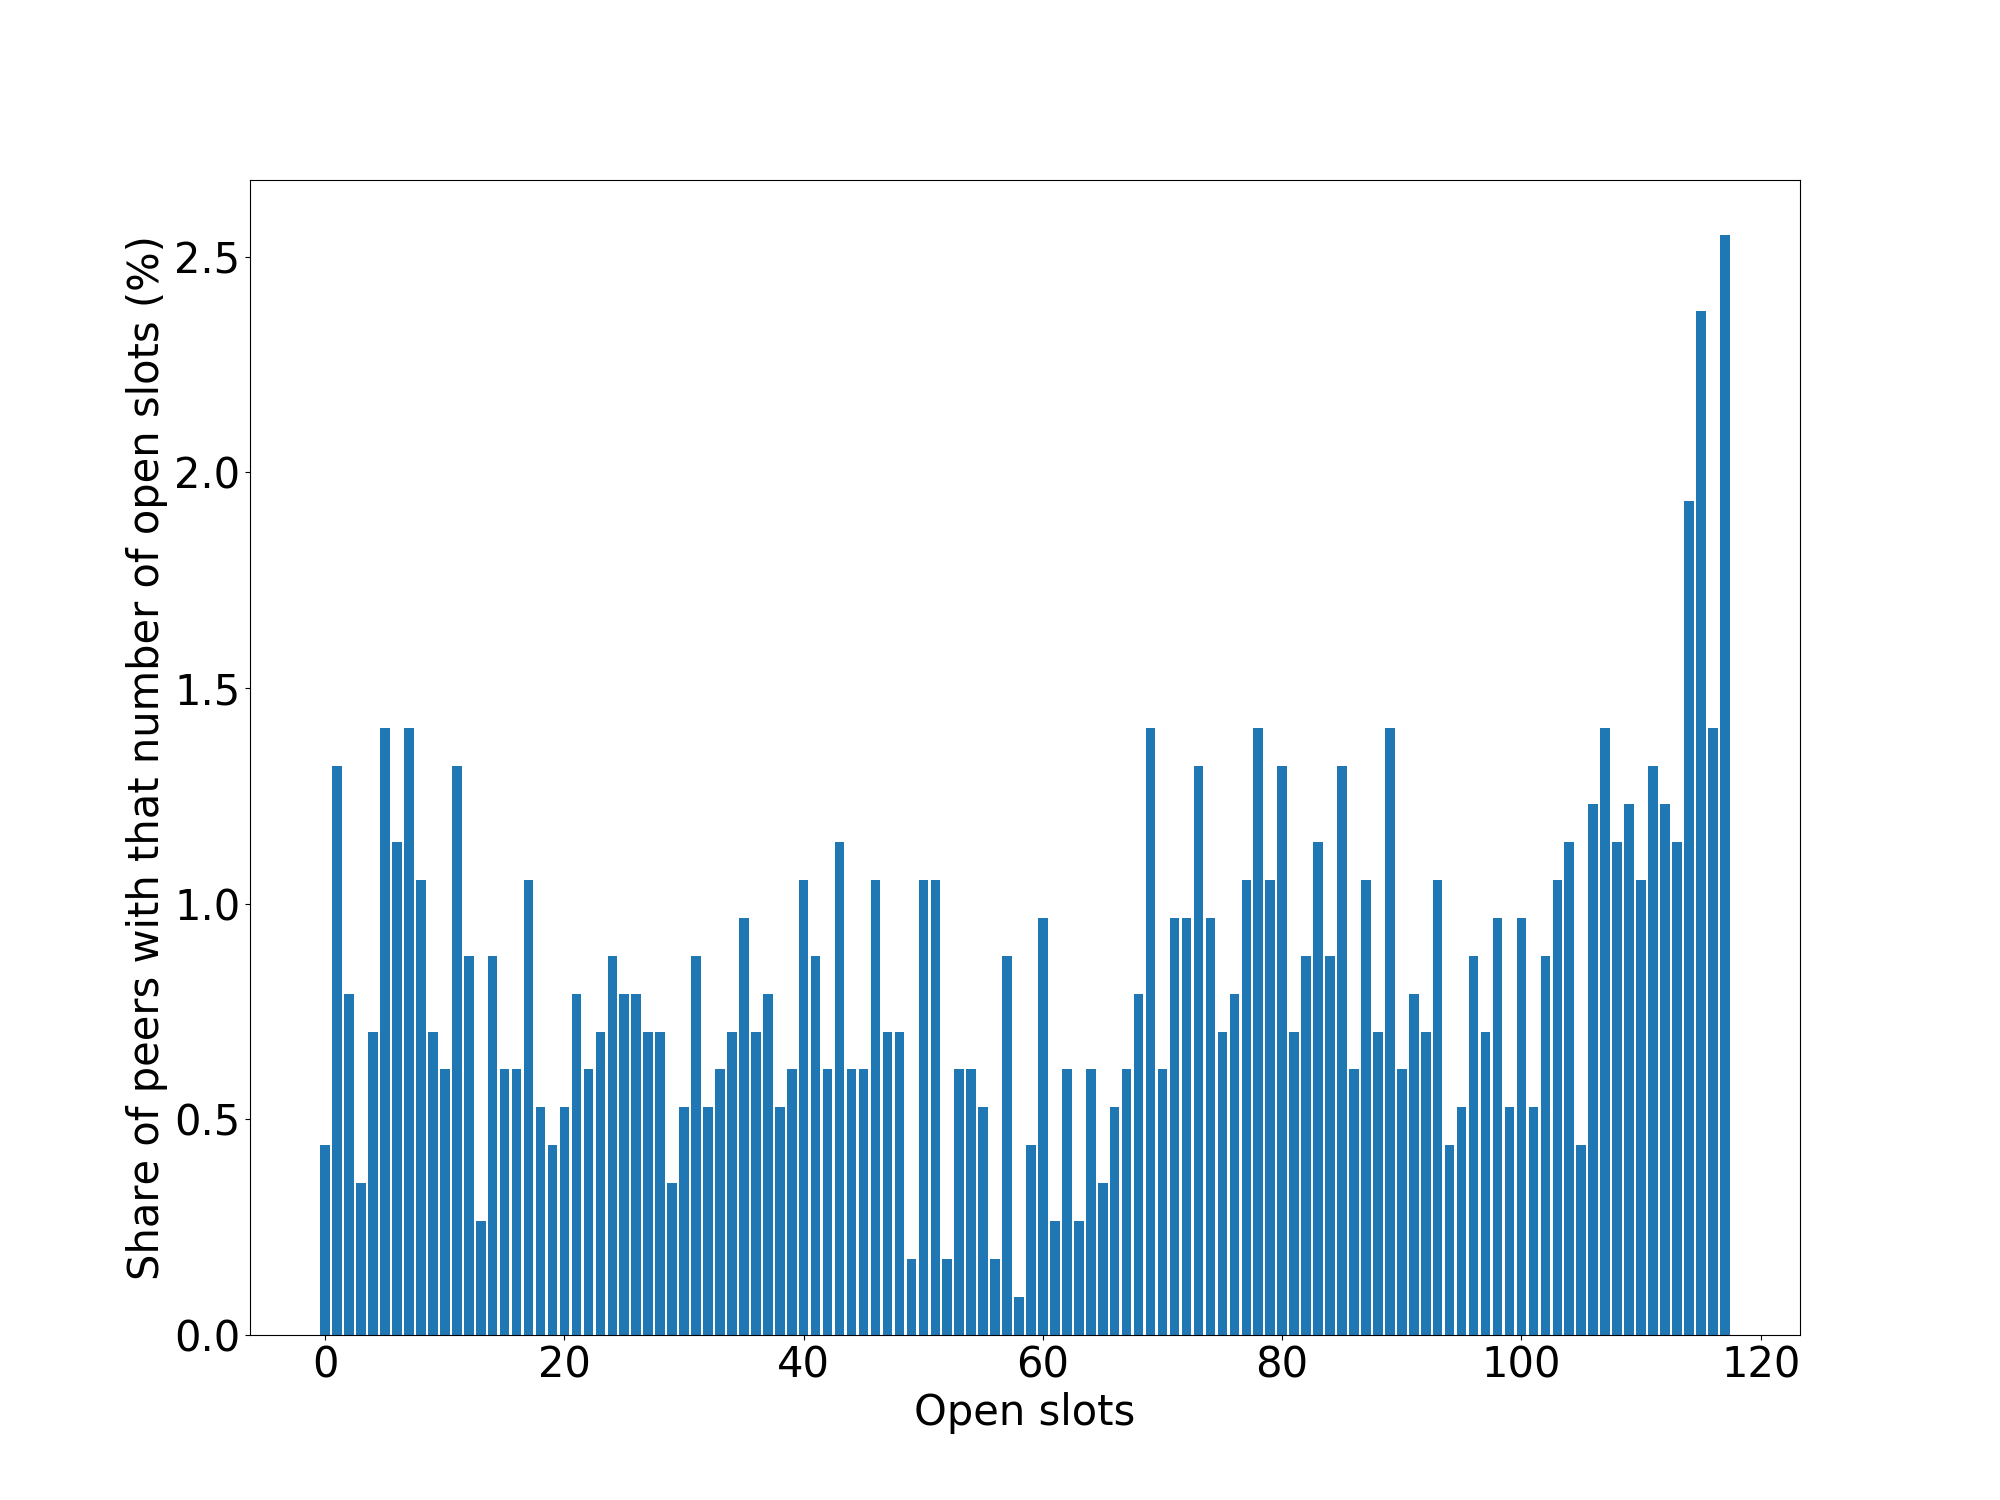
\includegraphics[width=\columnwidth]{bitcoin-testnet-1541513977-conn-max-histogram.png}
		\caption{Free connection slots for Bitcoin testnet.}
		\label{fig:free-slots-bitcoin}
	\end{minipage}\hfill
	\begin{minipage}{0.5\textwidth}
		\centering
		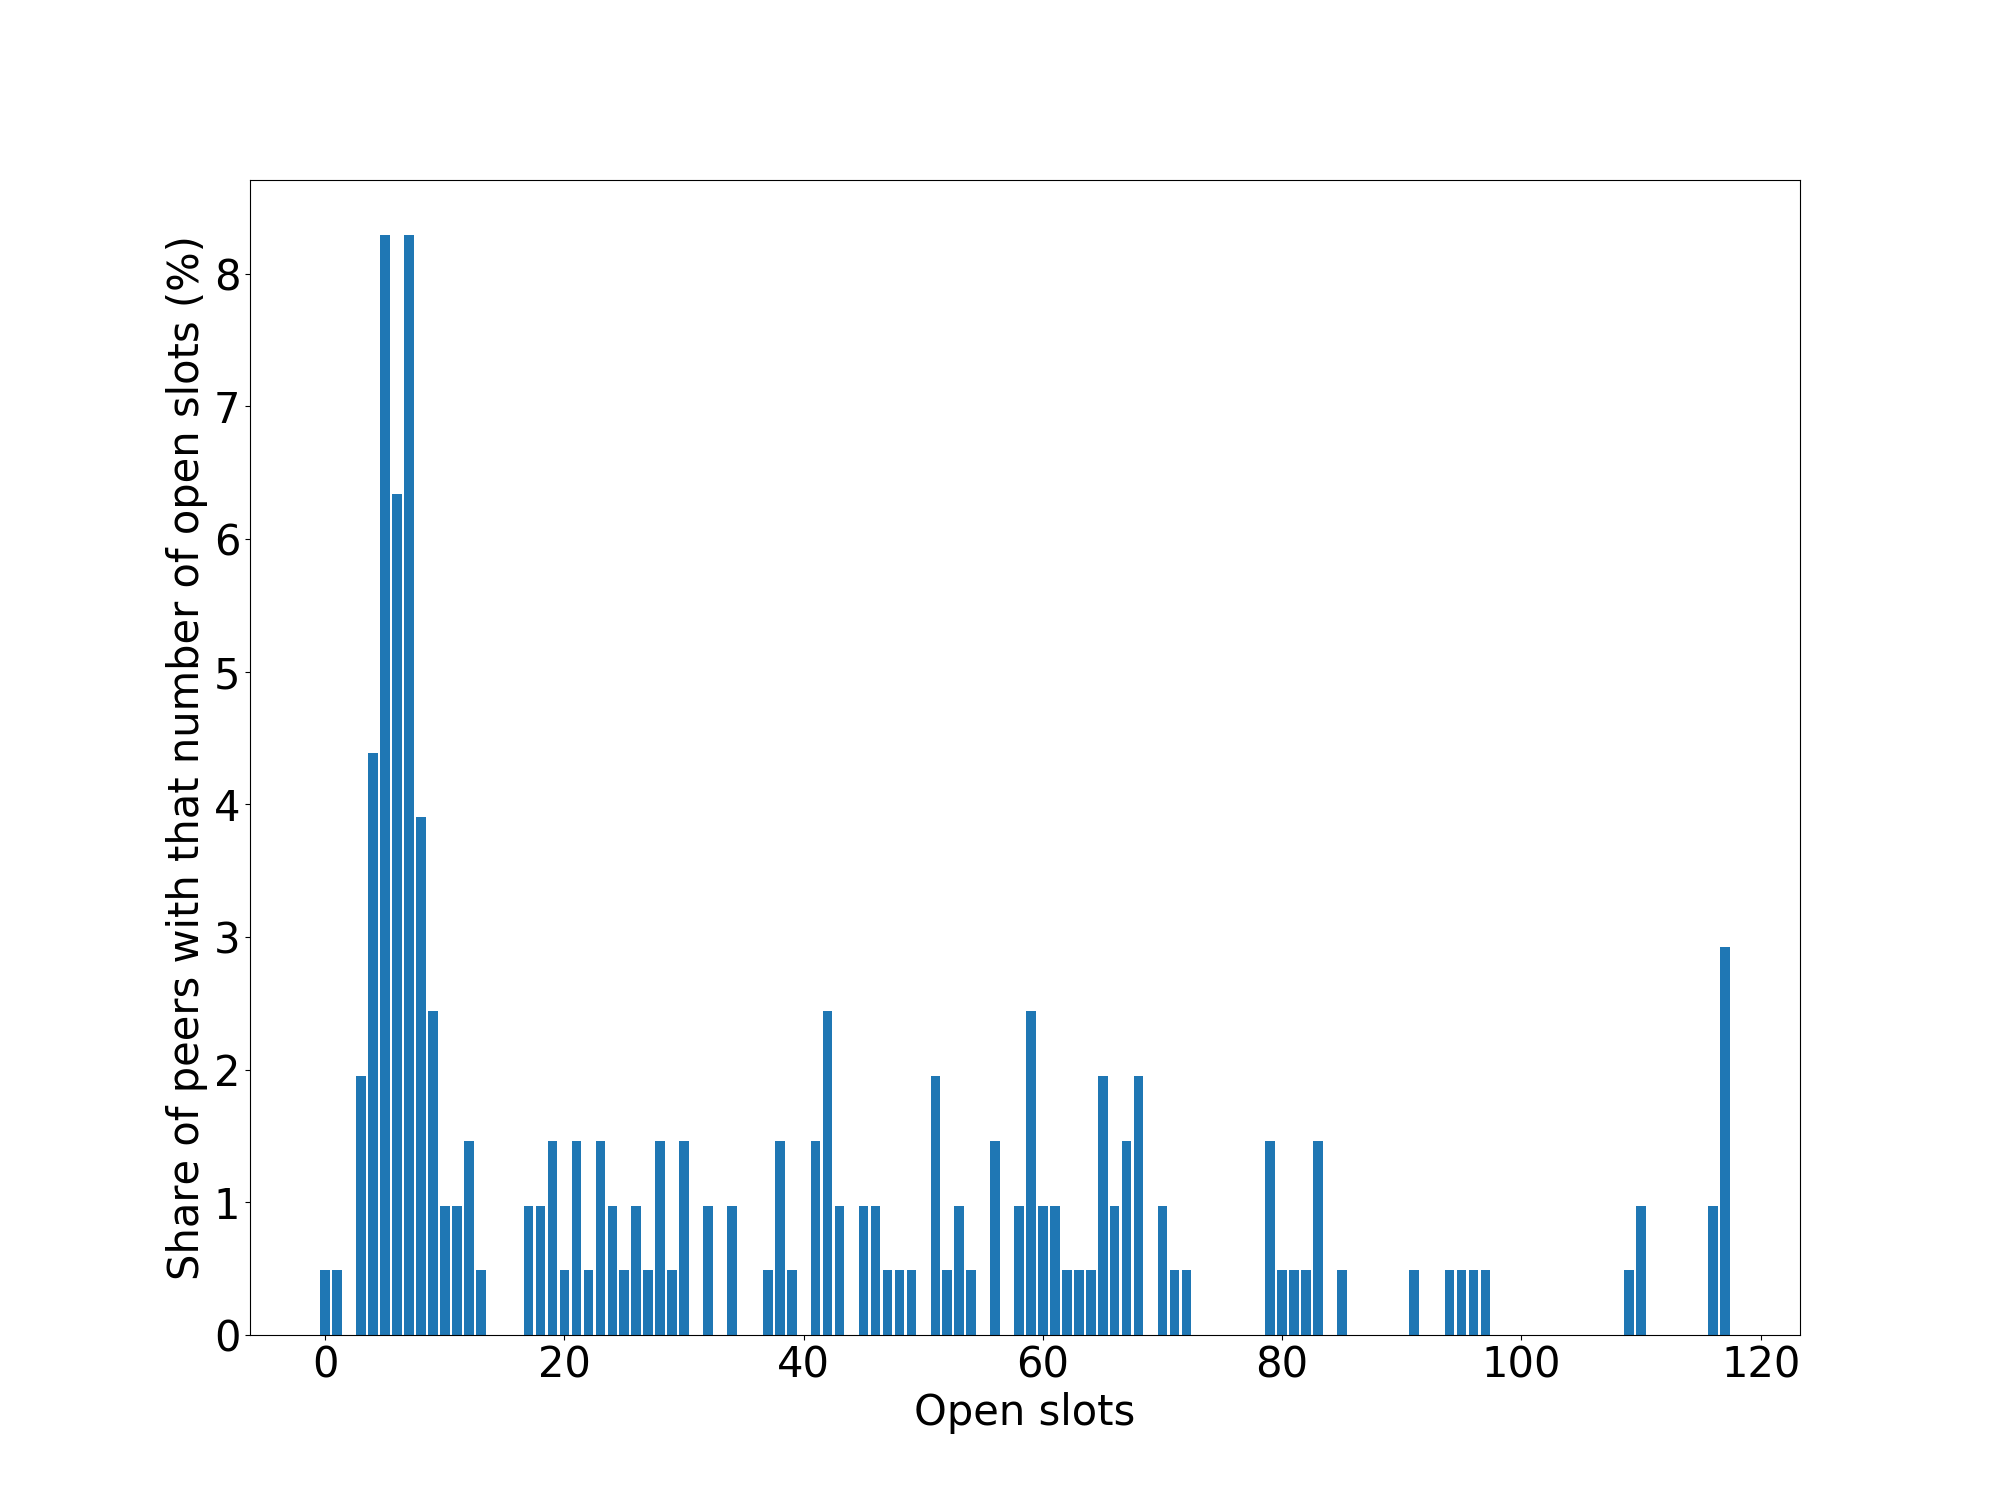
\includegraphics[width=\columnwidth]{zcash-mainnet-1541938472-conn-max-histogram.png}
		\caption{Free connection slots for Zcash mainnet.}
		\label{fig:free-slots-zcash}
	\end{minipage}\hfill
\end{figure*}


\subsubsection{Dash}

Dash is also based on the Bitcoin~Core codebase and inherits the basics of its networking protocol.
Dash uses diffusion for broadcast randomization.
The Dash networking protocol is substantially more complex compared with Bitcoin.
Dash contains $22$~new message types for masternode management~\cite{Schinzel2015}.
Masternode-related tasks include periodic pings to check whether masternodes are online, coin mixing and voting for governance proposals.
Our tool does not handle Dash-specific messages.

In our experiment, we connect to $500$~out of~$3\,065$~randomly chosen Dash nodes and ask for $30$~connection slots.
During $15$-minutes, we receive $12$~transaction inventory messages and~$396$~Dash-specific messages.

\begin{figure*}
	\centering
	\begin{minipage}{0.5\textwidth}
		\centering
		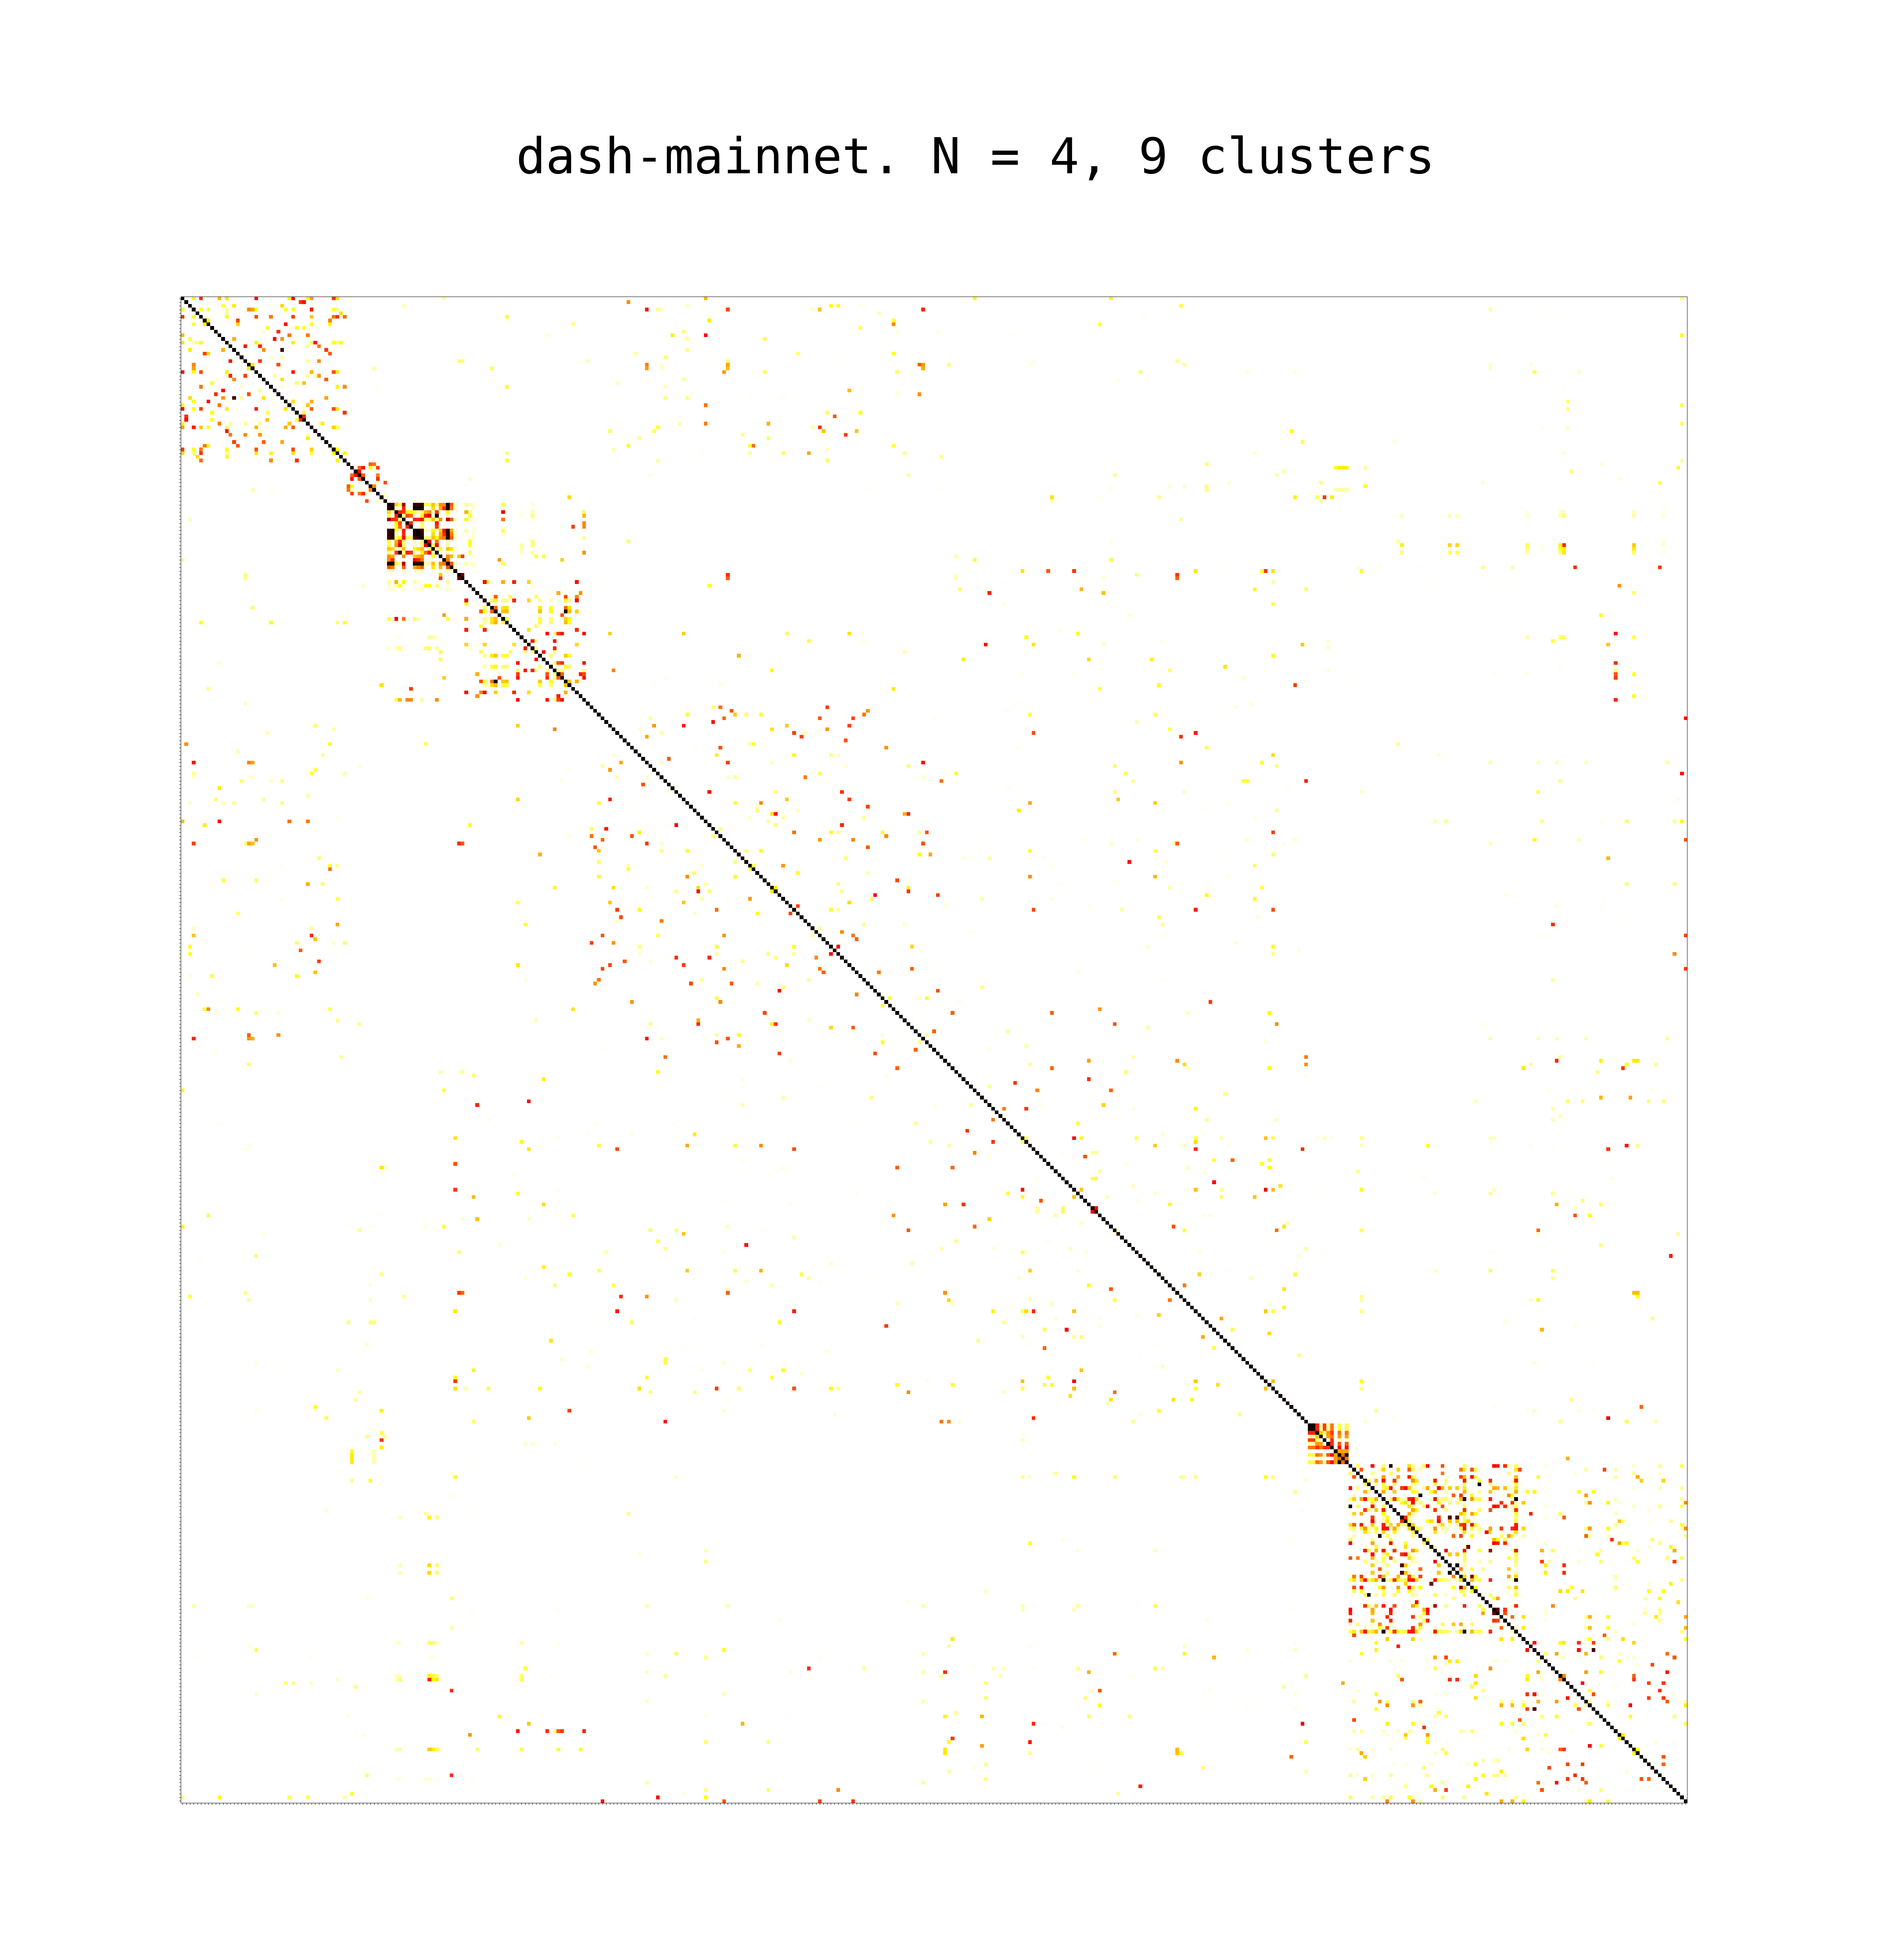
\includegraphics[width=\columnwidth]{dash-mainnet-1531510768-all.png}
		\caption{Transaction clustering for Dash (messages and transactions).}
		\label{fig:dash-all}
	\end{minipage}\hfill
	\begin{minipage}{0.5\textwidth}
		\centering
		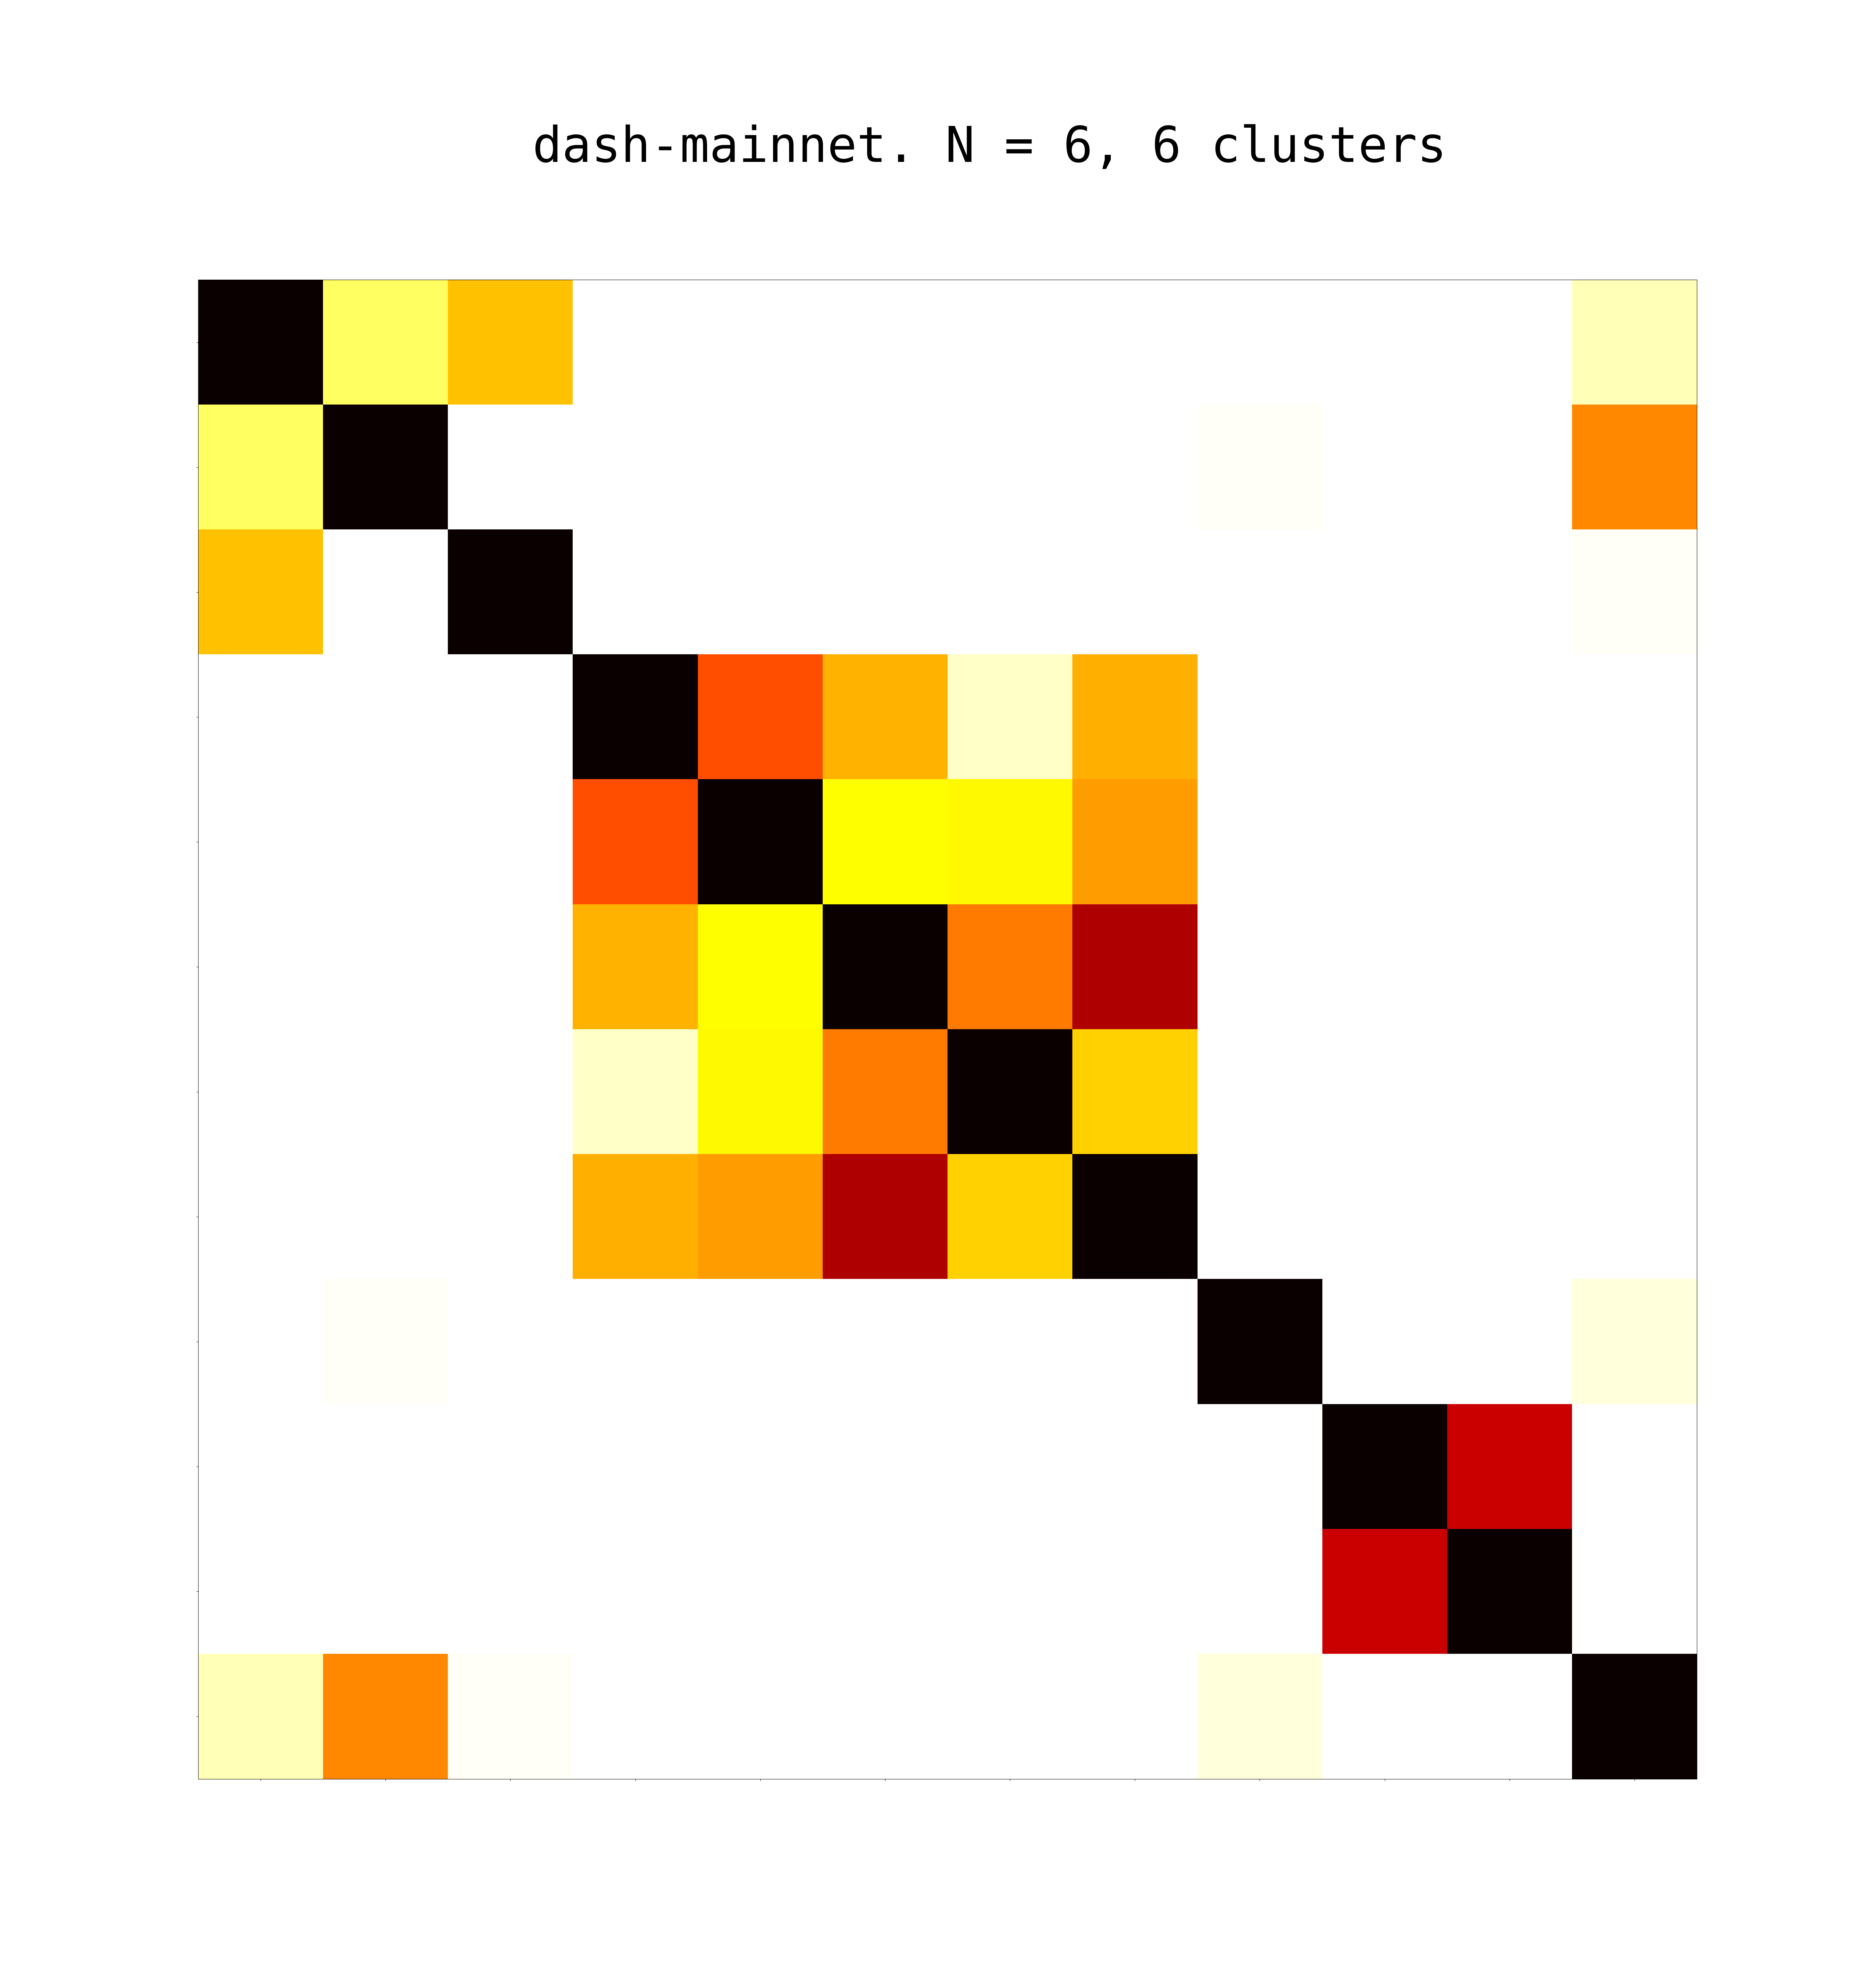
\includegraphics[width=\columnwidth]{dash-mainnet-1531510768.png}
		\caption{Transaction clustering for Dash (transactions only).}
		\label{fig:dash-tx}
	\end{minipage}\hfill
\end{figure*}

We run the clustering algorithm twice: accounting for the Dash-specific messages (Figure~\ref{fig:dash-all}), and considering only standard transaction inventory messages (Figure~\ref{fig:dash-tx}).
In both cases, we obtain clearly visible clusters.
These preliminary results show a privacy concern, especially if combined with transaction graph analysis~\cite{Kalodner2017}.


\subsubsection{Monero}

Monero is a privacy-focused cryptocurrency not based on the Bitcoin~Core codebase.
Monero provides privacy by default: users do not have to explicitly choose the "private" option, contrary to Zcash (shielded transactions) and Dash (\textit{PrivateSend}).

The Monero community recognizes the threat of deanonymization through network analysis~\cite{user36432017, manontheinside2016, expez2016, Cameron2016}.
This has motivated the integration of Dandelion++ networking protocol in 2020~\cite{ErCiccione2020} (see Section~\ref{sec:Dandelion}).
Moreover, the Kovri project~\cite{Kovri} aims to add an I2P router into Monero.
As of the time of our experiments (mid-2018), Monero uses no broadcast randomization.

Monero does not allow creating and spending a transaction output in the same block.
A new output appears as "locked" until the transaction that creates it receives $10$~confirmations ($20$~minutes at the target block time of~$2$~minutes)~\cite{dpzz2017}.
Though this is a wallet-level and not a protocol-level restriction, the official desktop wallet and Monerujo, a popular Monero wallet for Android, enforce it.
Therefore, the scenario of our earlier experiments is somewhat unrealistic.
For example, to issue $20$~transactions within a $20$~minute period, a user must have $20$~"unlocked" transaction outputs (each takes $20$~minutes to create).

We conduct an experiment on Monero without issuing transactions.
This experiment aims to detect a block-diagonal structure in the correlation matrix derived from real-world transactions.
We connect to $200$~nodes and receive $124$~transactions in a $38$~minute window (Figure~\ref{fig:monero}).

\begin{figure}[!t]
	\centering
	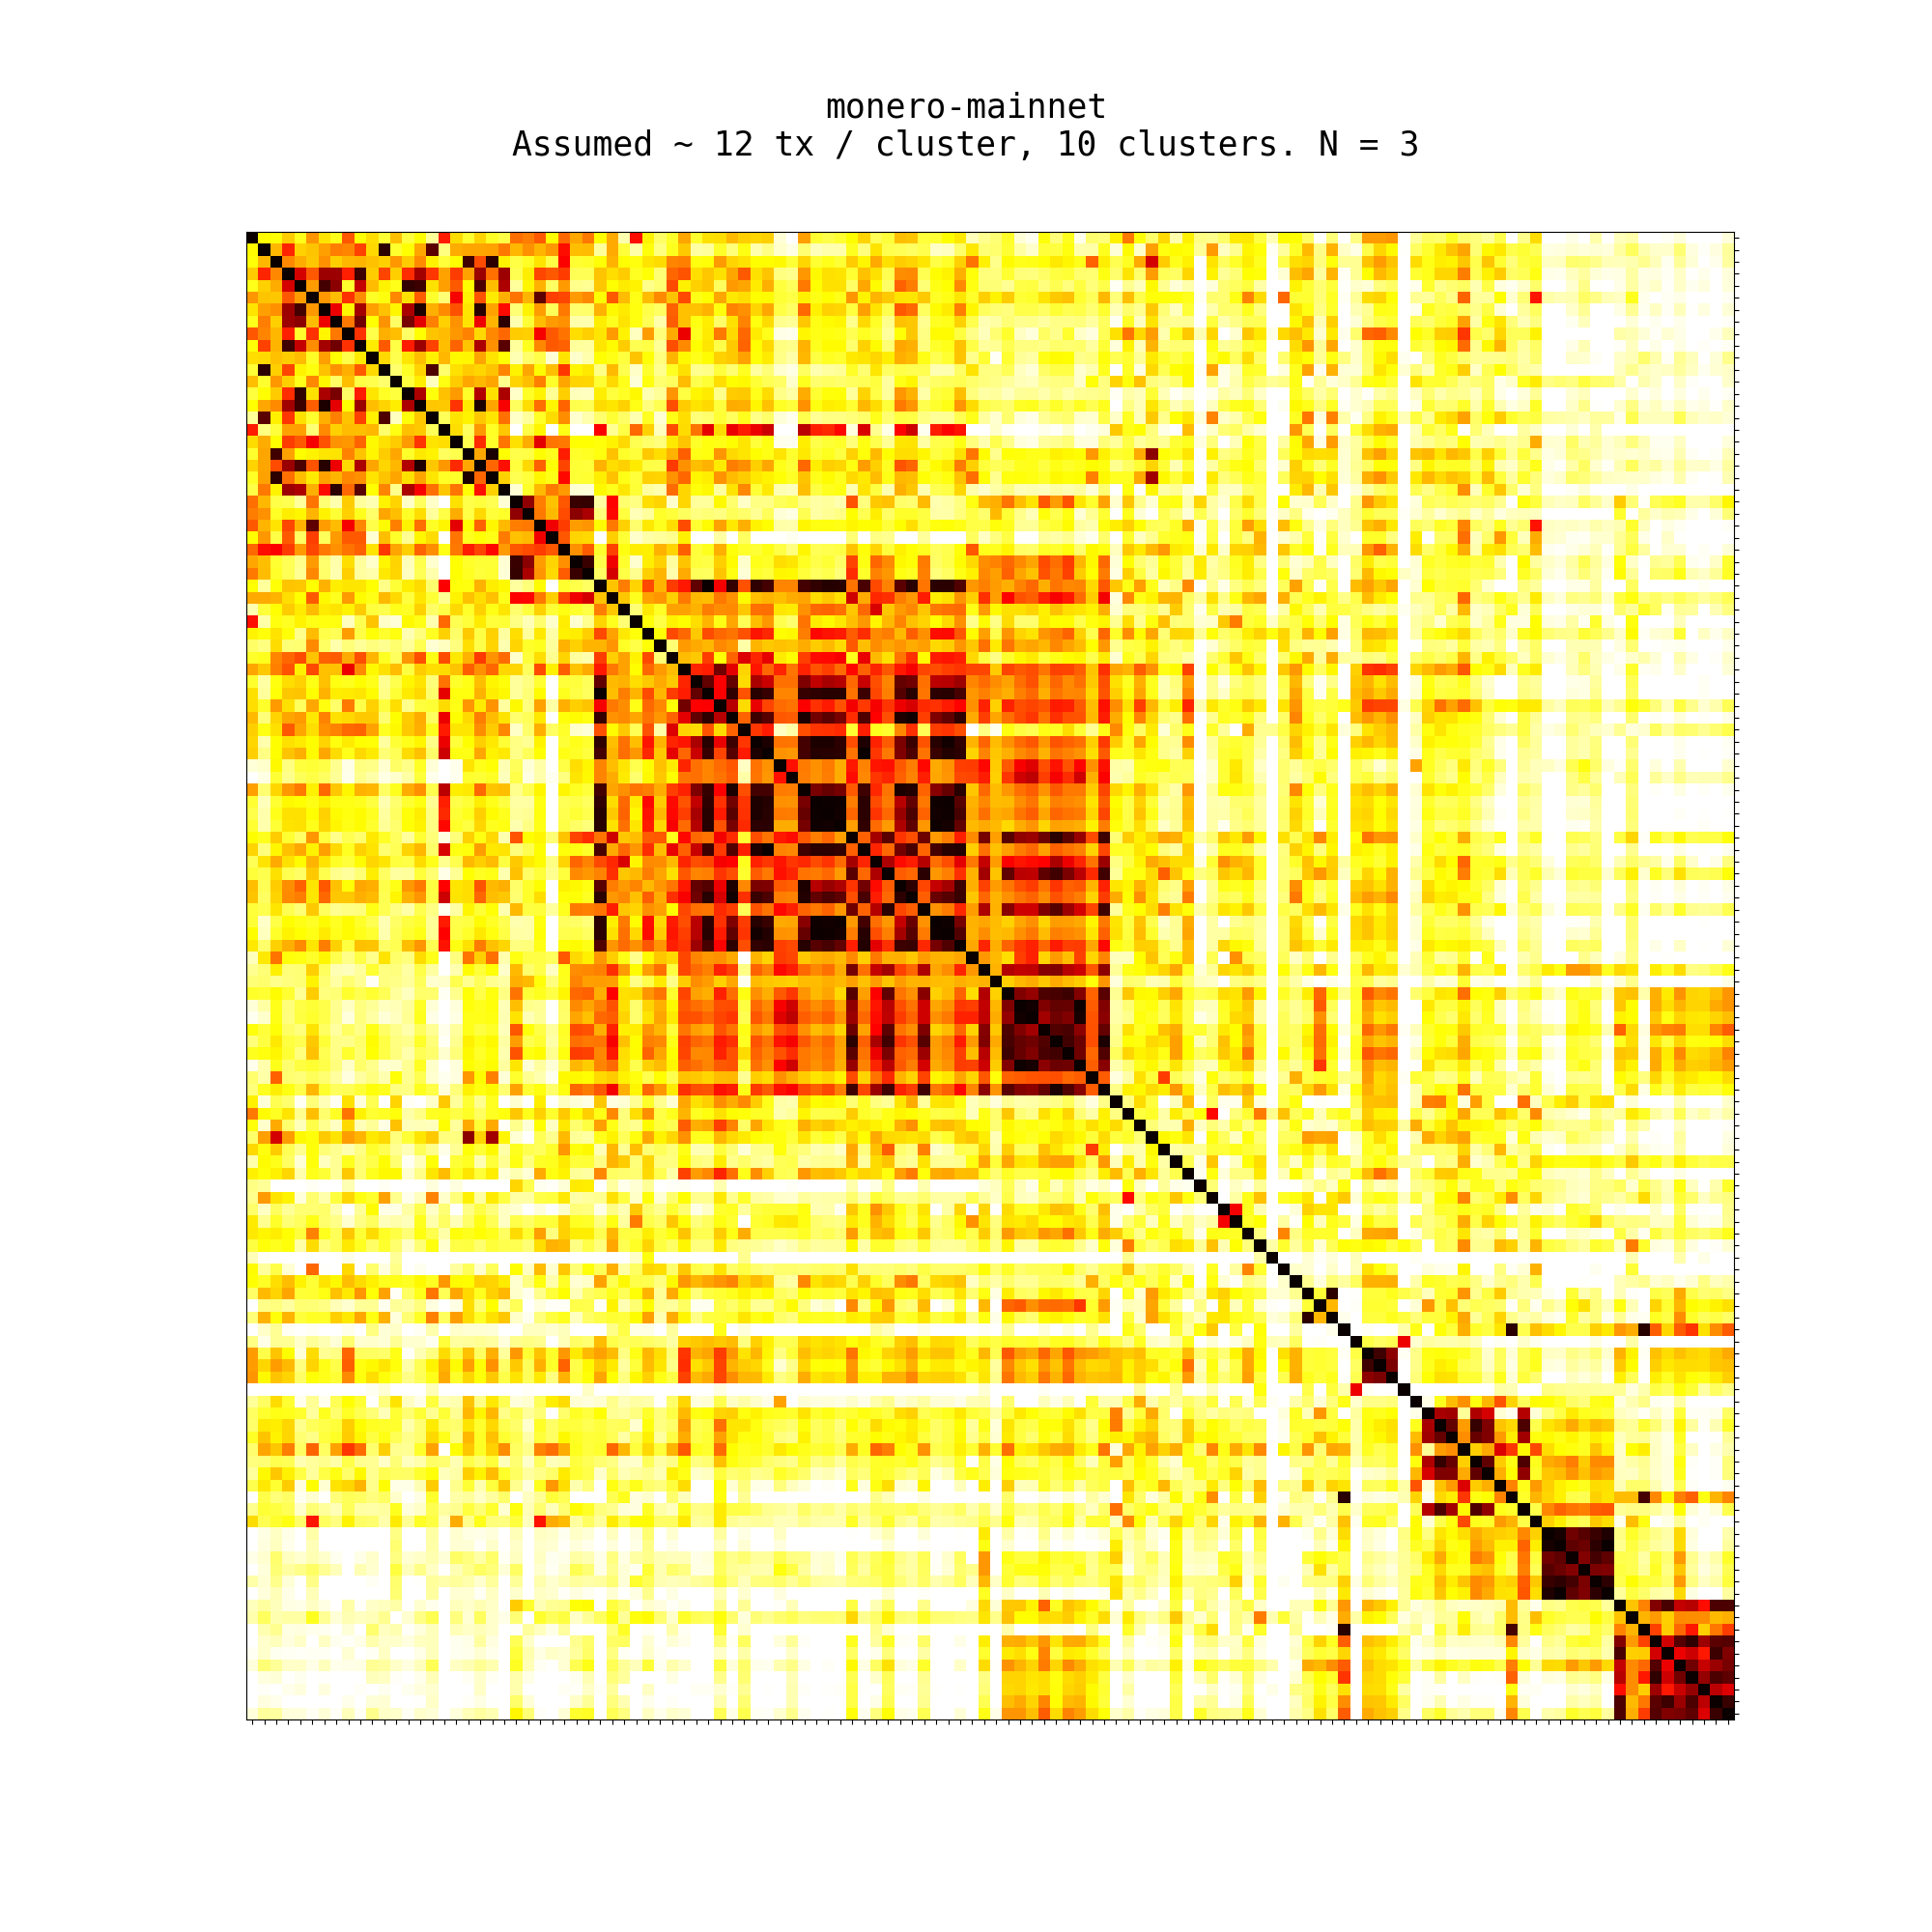
\includegraphics[width=0.5\columnwidth]{monero-mainnet-005-fig-correlations-012-txcl-003-N-Rand-best.png}
	\caption{Transaction clustering for Monero.}
	\label{fig:monero}
\end{figure}

We explain a less clear picture compared to the Bitcoin testnet as follows.
First, we connect to only~$200$ out of $1\,700$--$1\,800$ nodes (as of the time of the experiment~\cite{MoneroHash}).
Second, Monero does not use the three-step transaction propagation (\texttt{inv} -- \texttt{getdata} -- \texttt{tx}), which may have opposite effects on clustering quality.
On the one hand, relaying a transaction unconditionally to all neighbors increases the probability that we receive a new transaction from a node other than the source of one of its entry nodes.
On the other hand, this broadcast type may provide a near-perfect insight into transaction sources, if the attacker connects to all or nearly all nodes.
Third, \texttt{monerod} connects to nodes slower than \texttt{bcclient}, which impedes data collection.
In our experiment, while trying to connect to $200$~nodes, we obtain $150$~connections after approximately $2$~hours, $175$~connections after $3$~hours, $200$~connections after nearly $8$~hours.

Monero uses hard-coded DNS seeds and seed IP addresses for bootstrapping (see Chapter~\ref{sec:BitcoinP2PProtocol}).
As of July~2018, all DNS seeds fail to resolve.
The official client falls back to seed IP addresses.


\subsection{Results for mobile wallets}

We perform analogous experiments on Bitcoin (testnet and mainnet) and Zcash issuing transactions from selected mobile wallets for Android.
Most mobile wallets connect to the P2P network via a trusted server maintained by the wallet's developers.
We refer to wallets that connect to the P2P network directly as \textit{P2P wallets}.
Most P2P wallets rely on the BitcoinJ library for networking.
None of them uses broadcast randomization.
Unlike Bitcoin~Core, BitcoinJ sends \texttt{tx} unconditionally.\footnote{Note that in this case a full node receiving a \texttt{tx} message from an SPV node can be sure that the transaction originates at that SPV node, whereas receiving an \texttt{inv} announcement from a full node may also be a re-broadcast. This demonstrates the privacy enhancement of exclusively connecting to a trusted node for SPV.}
The BitcoinJ developers acknowledge that the three-step \texttt{inv} -- \texttt{getdata} -- \texttt{tx} exchange in Bitcoin~Core improves privacy, but argue that since SPV nodes have a weaker privacy model, the three-step broadcast would only decrease efficiency.

We choose a diverse selection of mobile wallets for our experiments: Bitcoin-only and multi-coin, with centralized and P2P networking.
We perform experiments on the Bitcoin testnet (Bitcoin wallet), the Bitcoin mainnet (Bitcoin wallet, BRD, Coinomi, Mycelium), and Zcash (Coinomi).
Bitcoin wallet and BRD\footnote{Bitcoin wallet and BRD are the two most popular Bitcoin clients~\cite{Wang2017}.} use P2P broadcast.
Coinomi and Mycelium use centralized broadcast.
For wallets with centralized broadcast, we only issue one set of transactions, using it as a "label" for a presumed wallet cluster.
If our transactions form a visible cluster, we inspect the IP addresses of nodes among the first ones to broadcast them.
Thus we infer the IP addresses of nodes likely to be used for transaction broadcasts for this wallet.
This information allows us to associate subsequent transactions with popular wallets.

\begin{figure}
	\centering
	\begin{subfigure}{.5\textwidth}
		\centering
		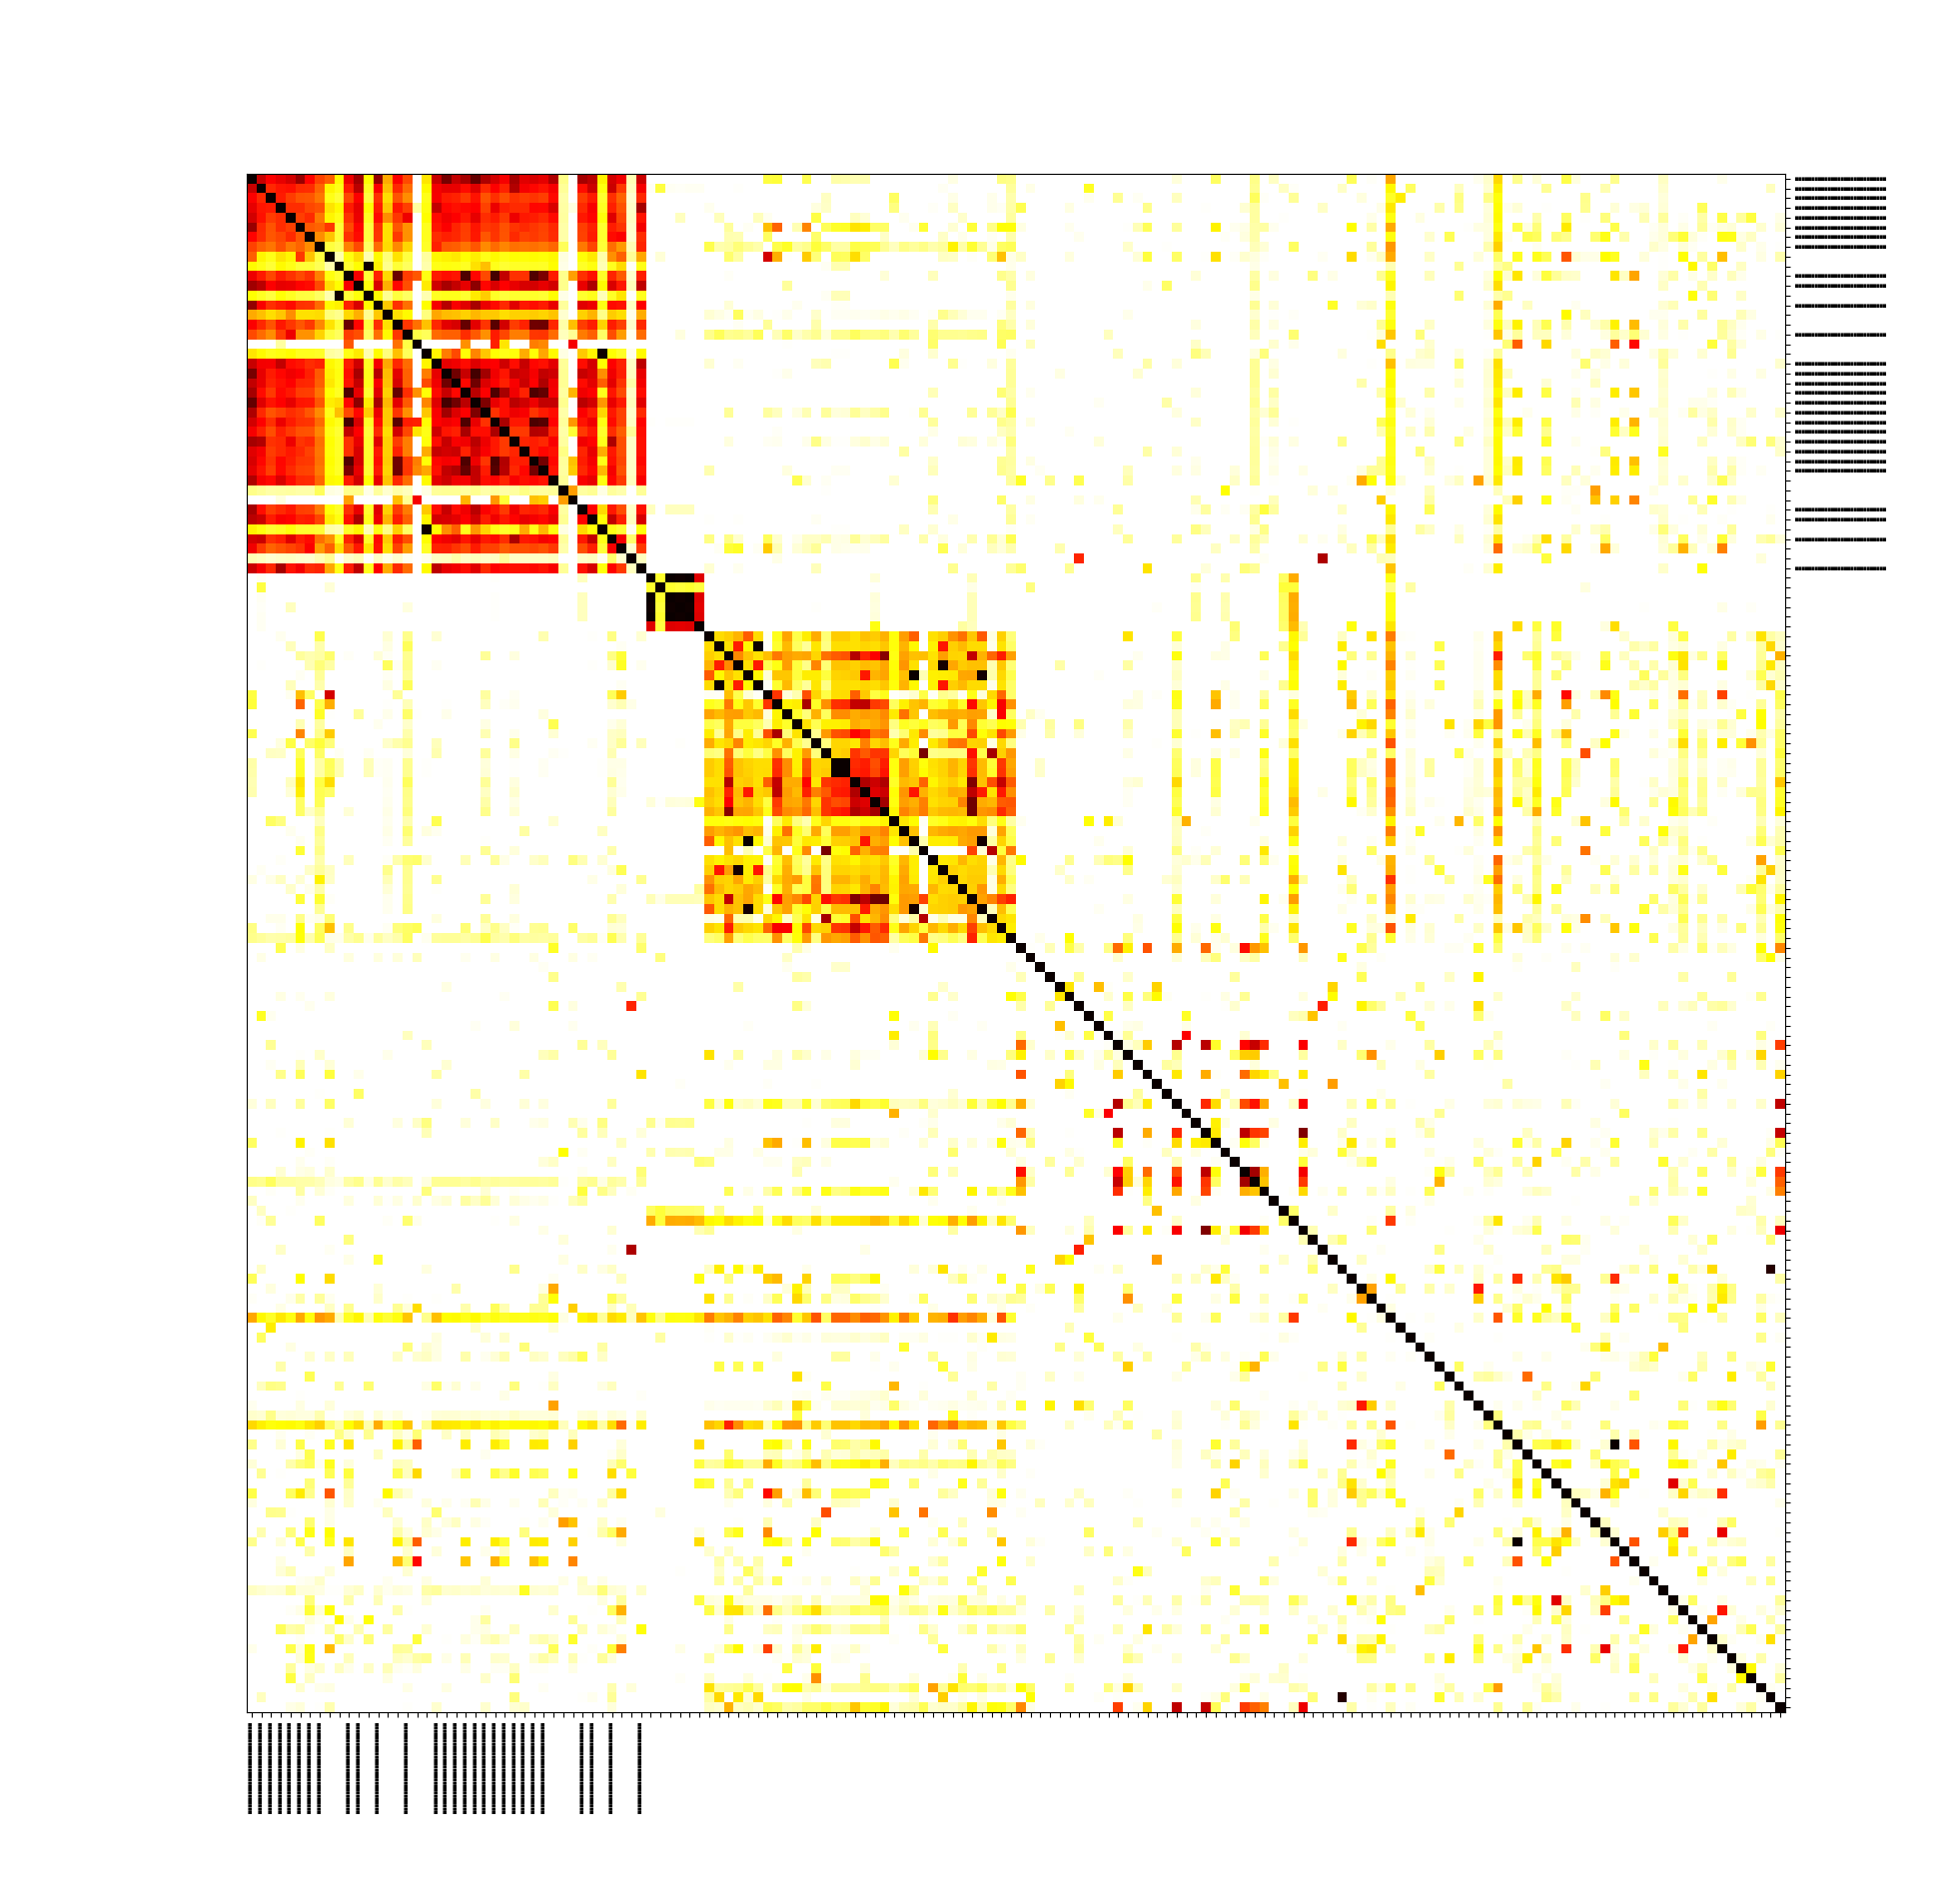
\includegraphics[width=\columnwidth]{bitcoin-testnet-1542895555-fig-corr-032-txcl-005-N-Rand.png}
		\caption{Bitcoin testnet, Mycelium.}
	\end{subfigure}%
	\begin{subfigure}{.5\textwidth}
		\centering
		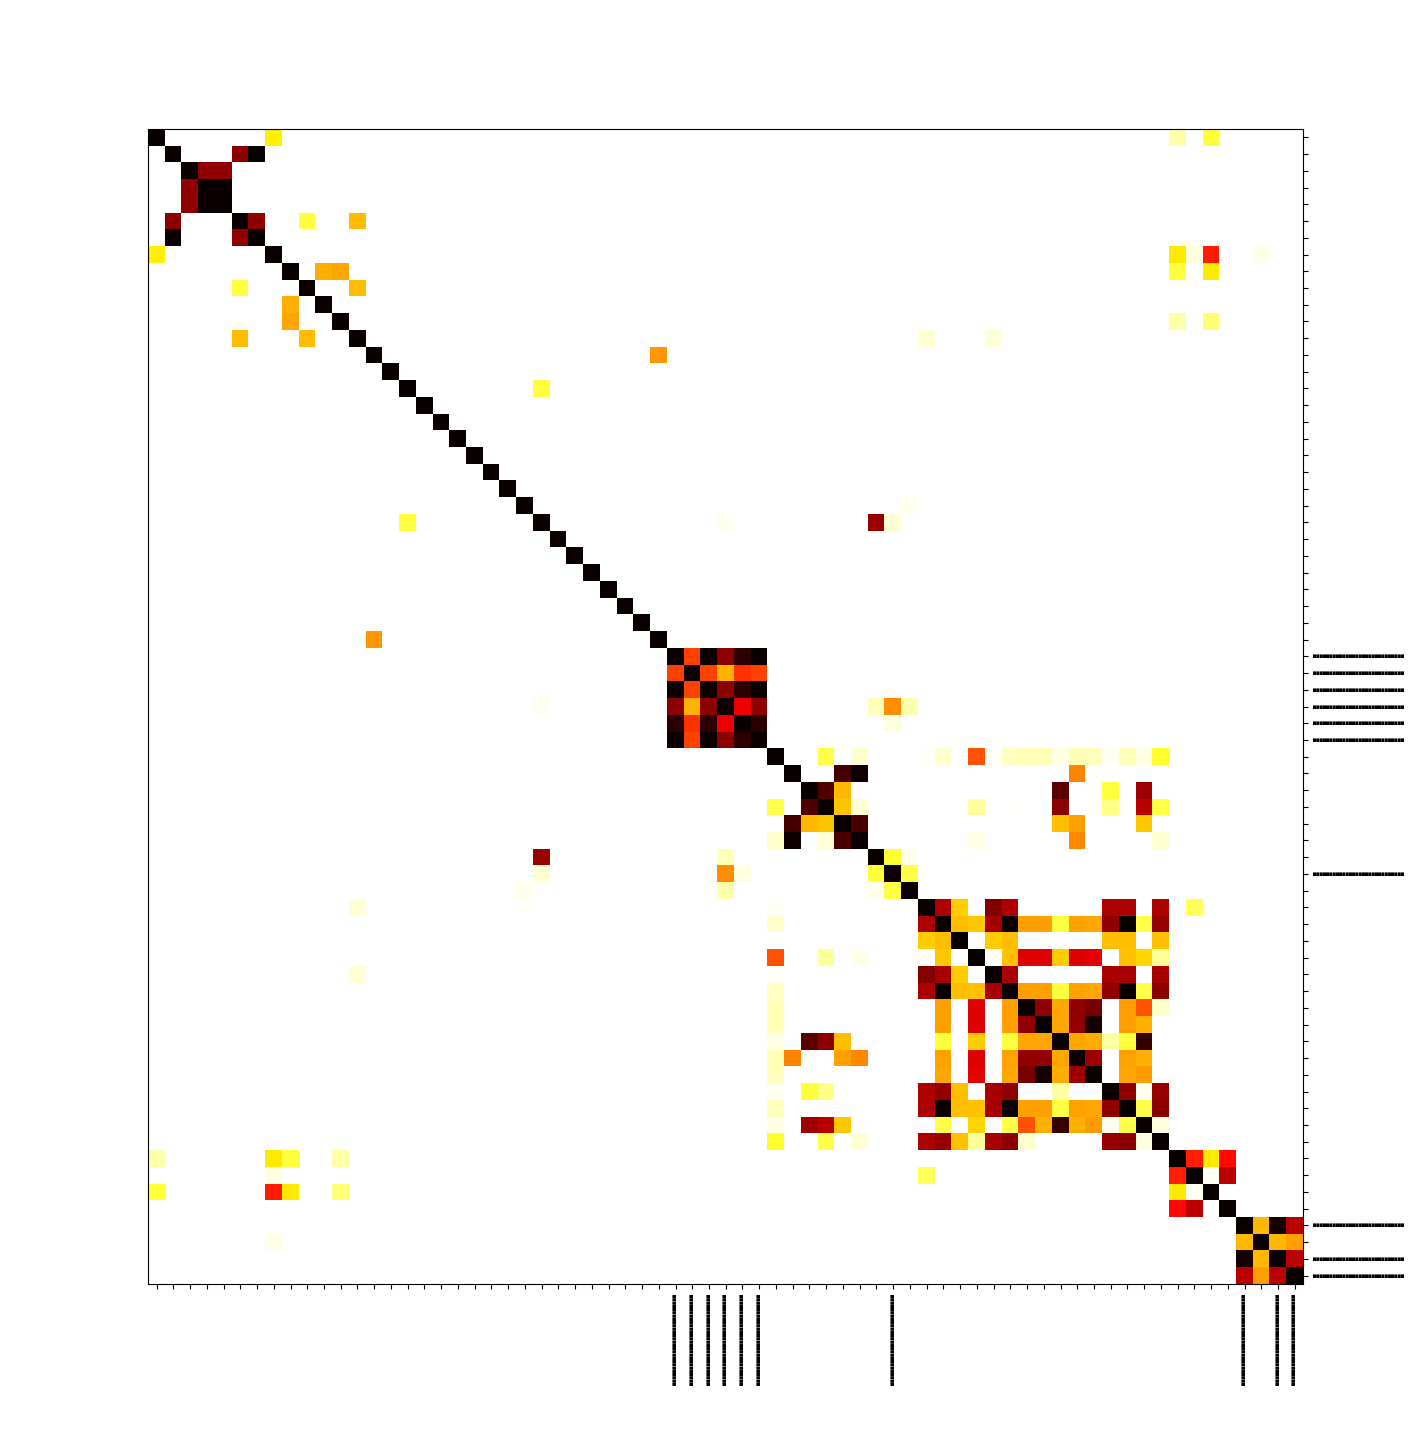
\includegraphics[width=\columnwidth]{bitcoin-testnet-1537202356-fig-corr-008-txcl-003-N-Rand.png}
		\caption{Bitcoin testnet, Bitcoin wallet.}
	\end{subfigure}
	\begin{subfigure}{.5\textwidth}
		\centering
		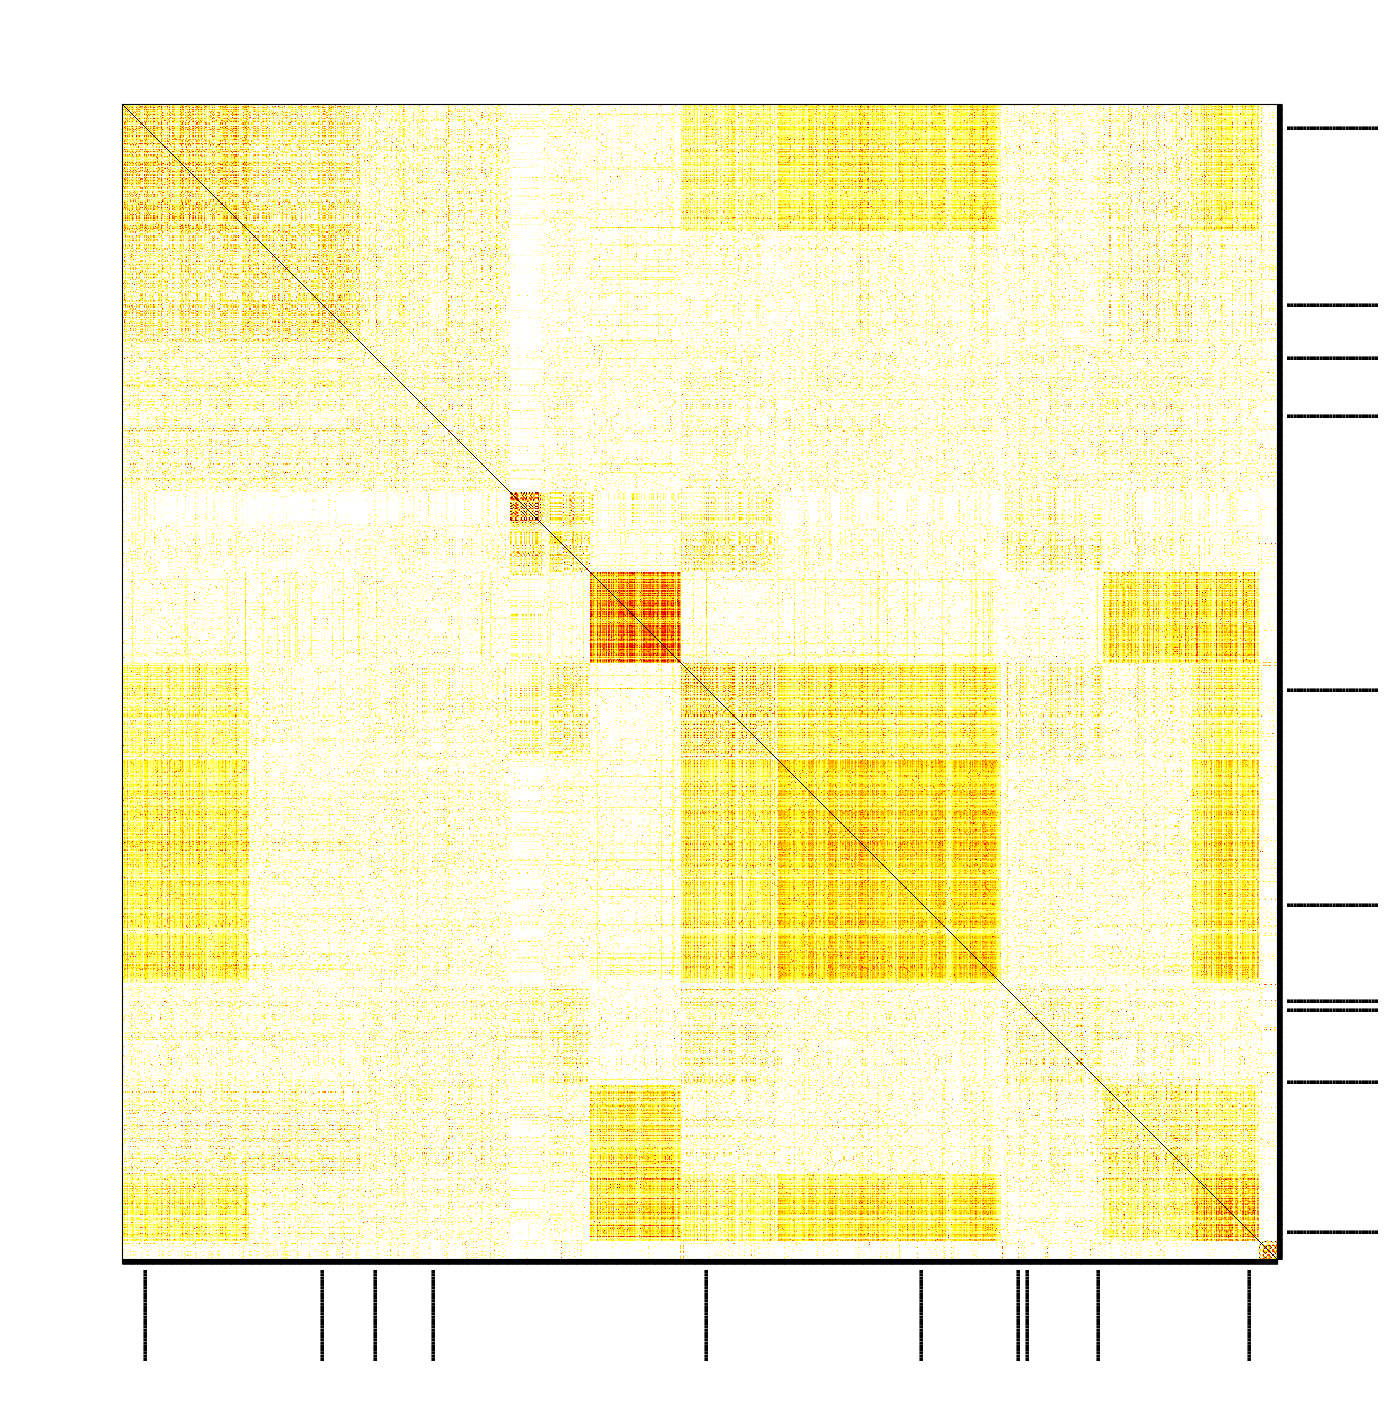
\includegraphics[width=\columnwidth]{bitcoin-mainnet-1537365306-fig-corr-202-txcl-007-N-Rand.png}
		\caption{Bitcoin mainnet, Bitcoin wallet.}
	\end{subfigure}%
	\begin{subfigure}{.5\textwidth}
		\centering
		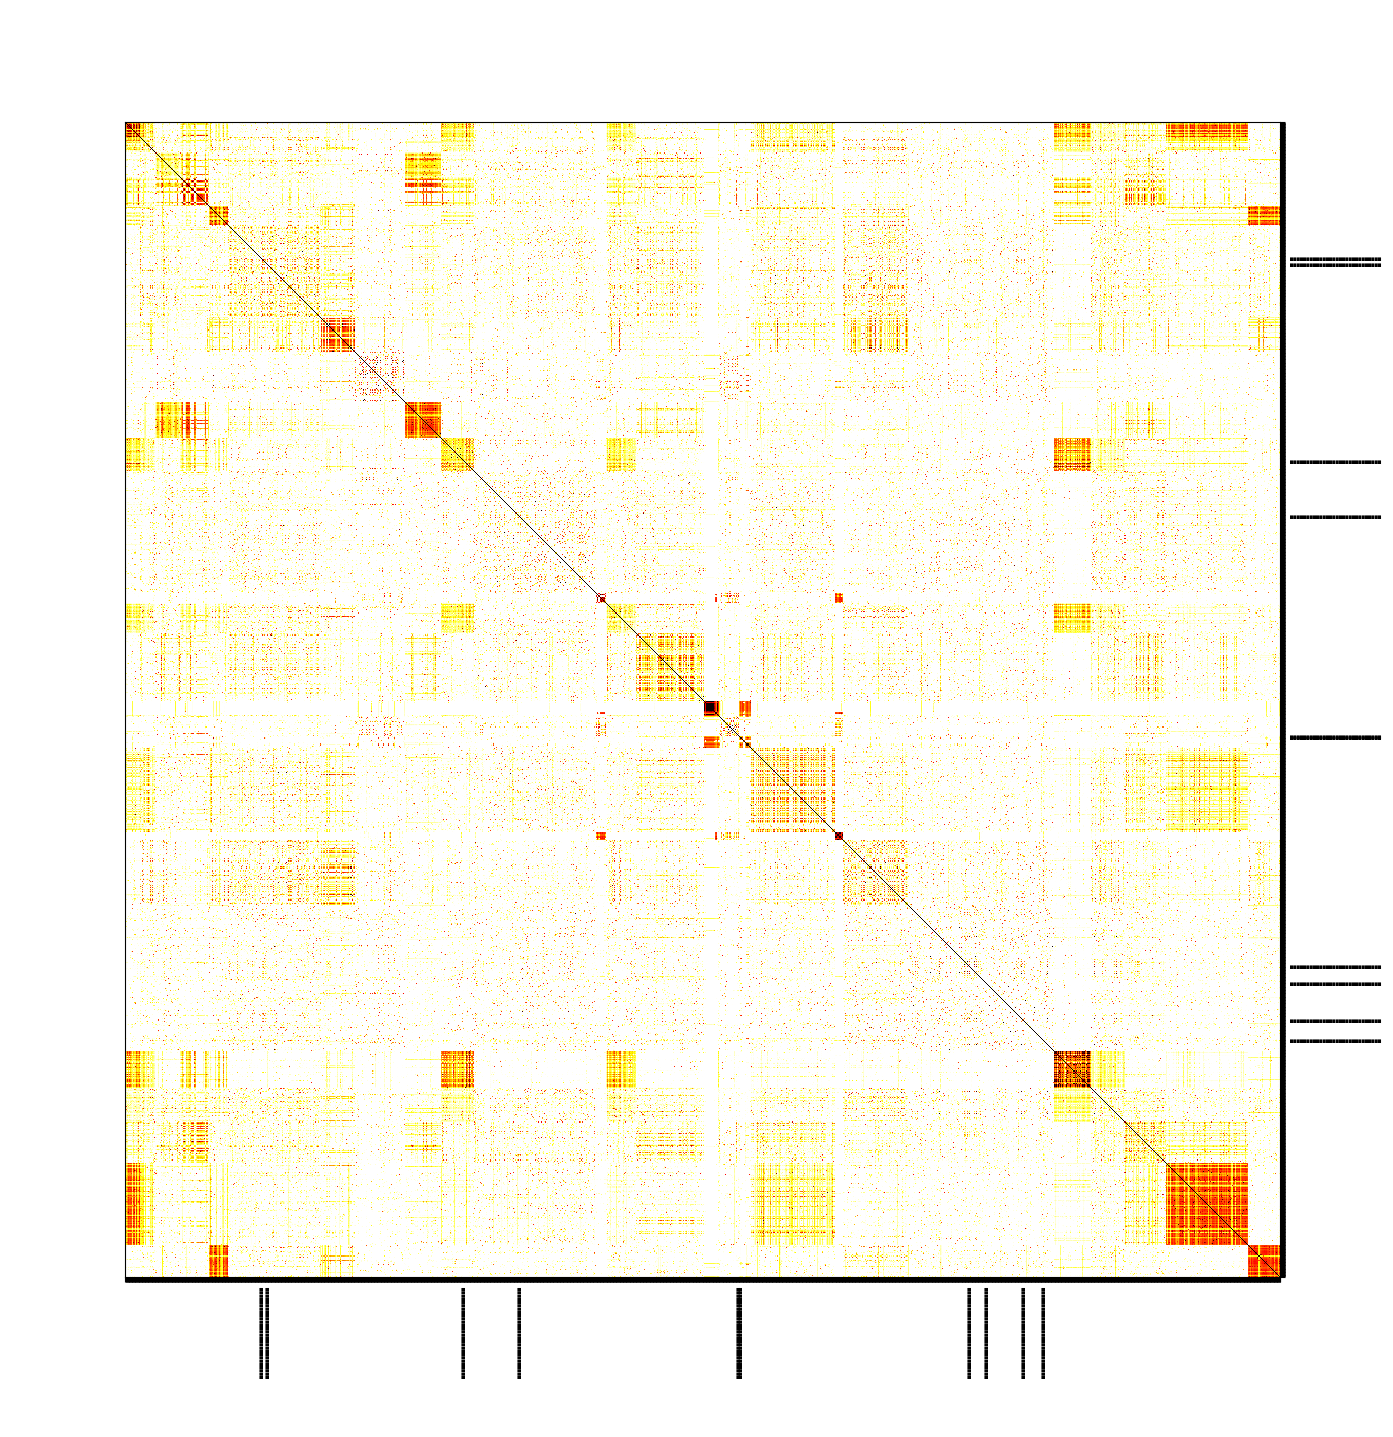
\includegraphics[width=\columnwidth]{bitcoin-mainnet-1537377559-fig-corr-102-txcl-004-N-Rand.png}
		\caption{Bitcoin mainnet, BRD.}
	\end{subfigure}
	\begin{subfigure}{.5\textwidth}
		\centering
		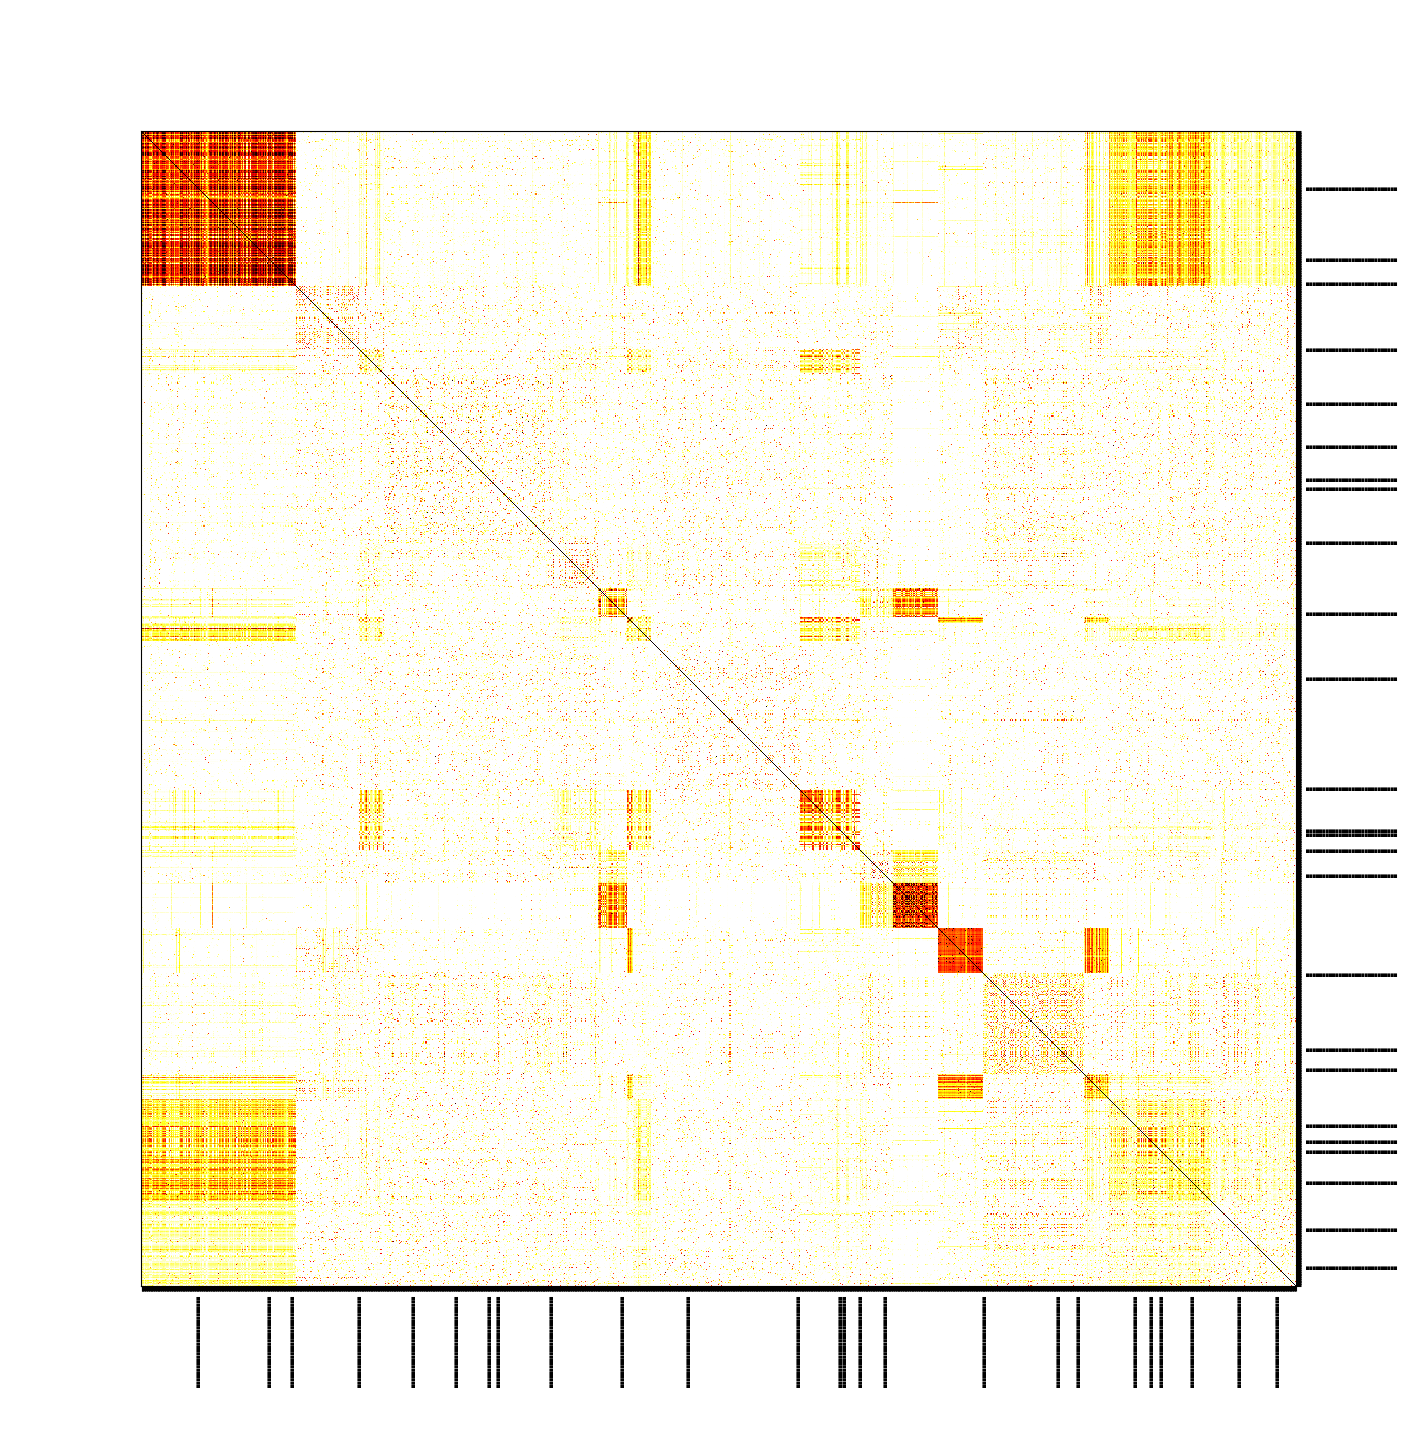
\includegraphics[width=\columnwidth]{bitcoin-mainnet-1537951300-fig-corr-100-txcl-004-N-Rand.png}
		\caption{Bitcoin mainnet, Coinomi.}
	\end{subfigure}%
	\begin{subfigure}{.5\textwidth}
		\centering
		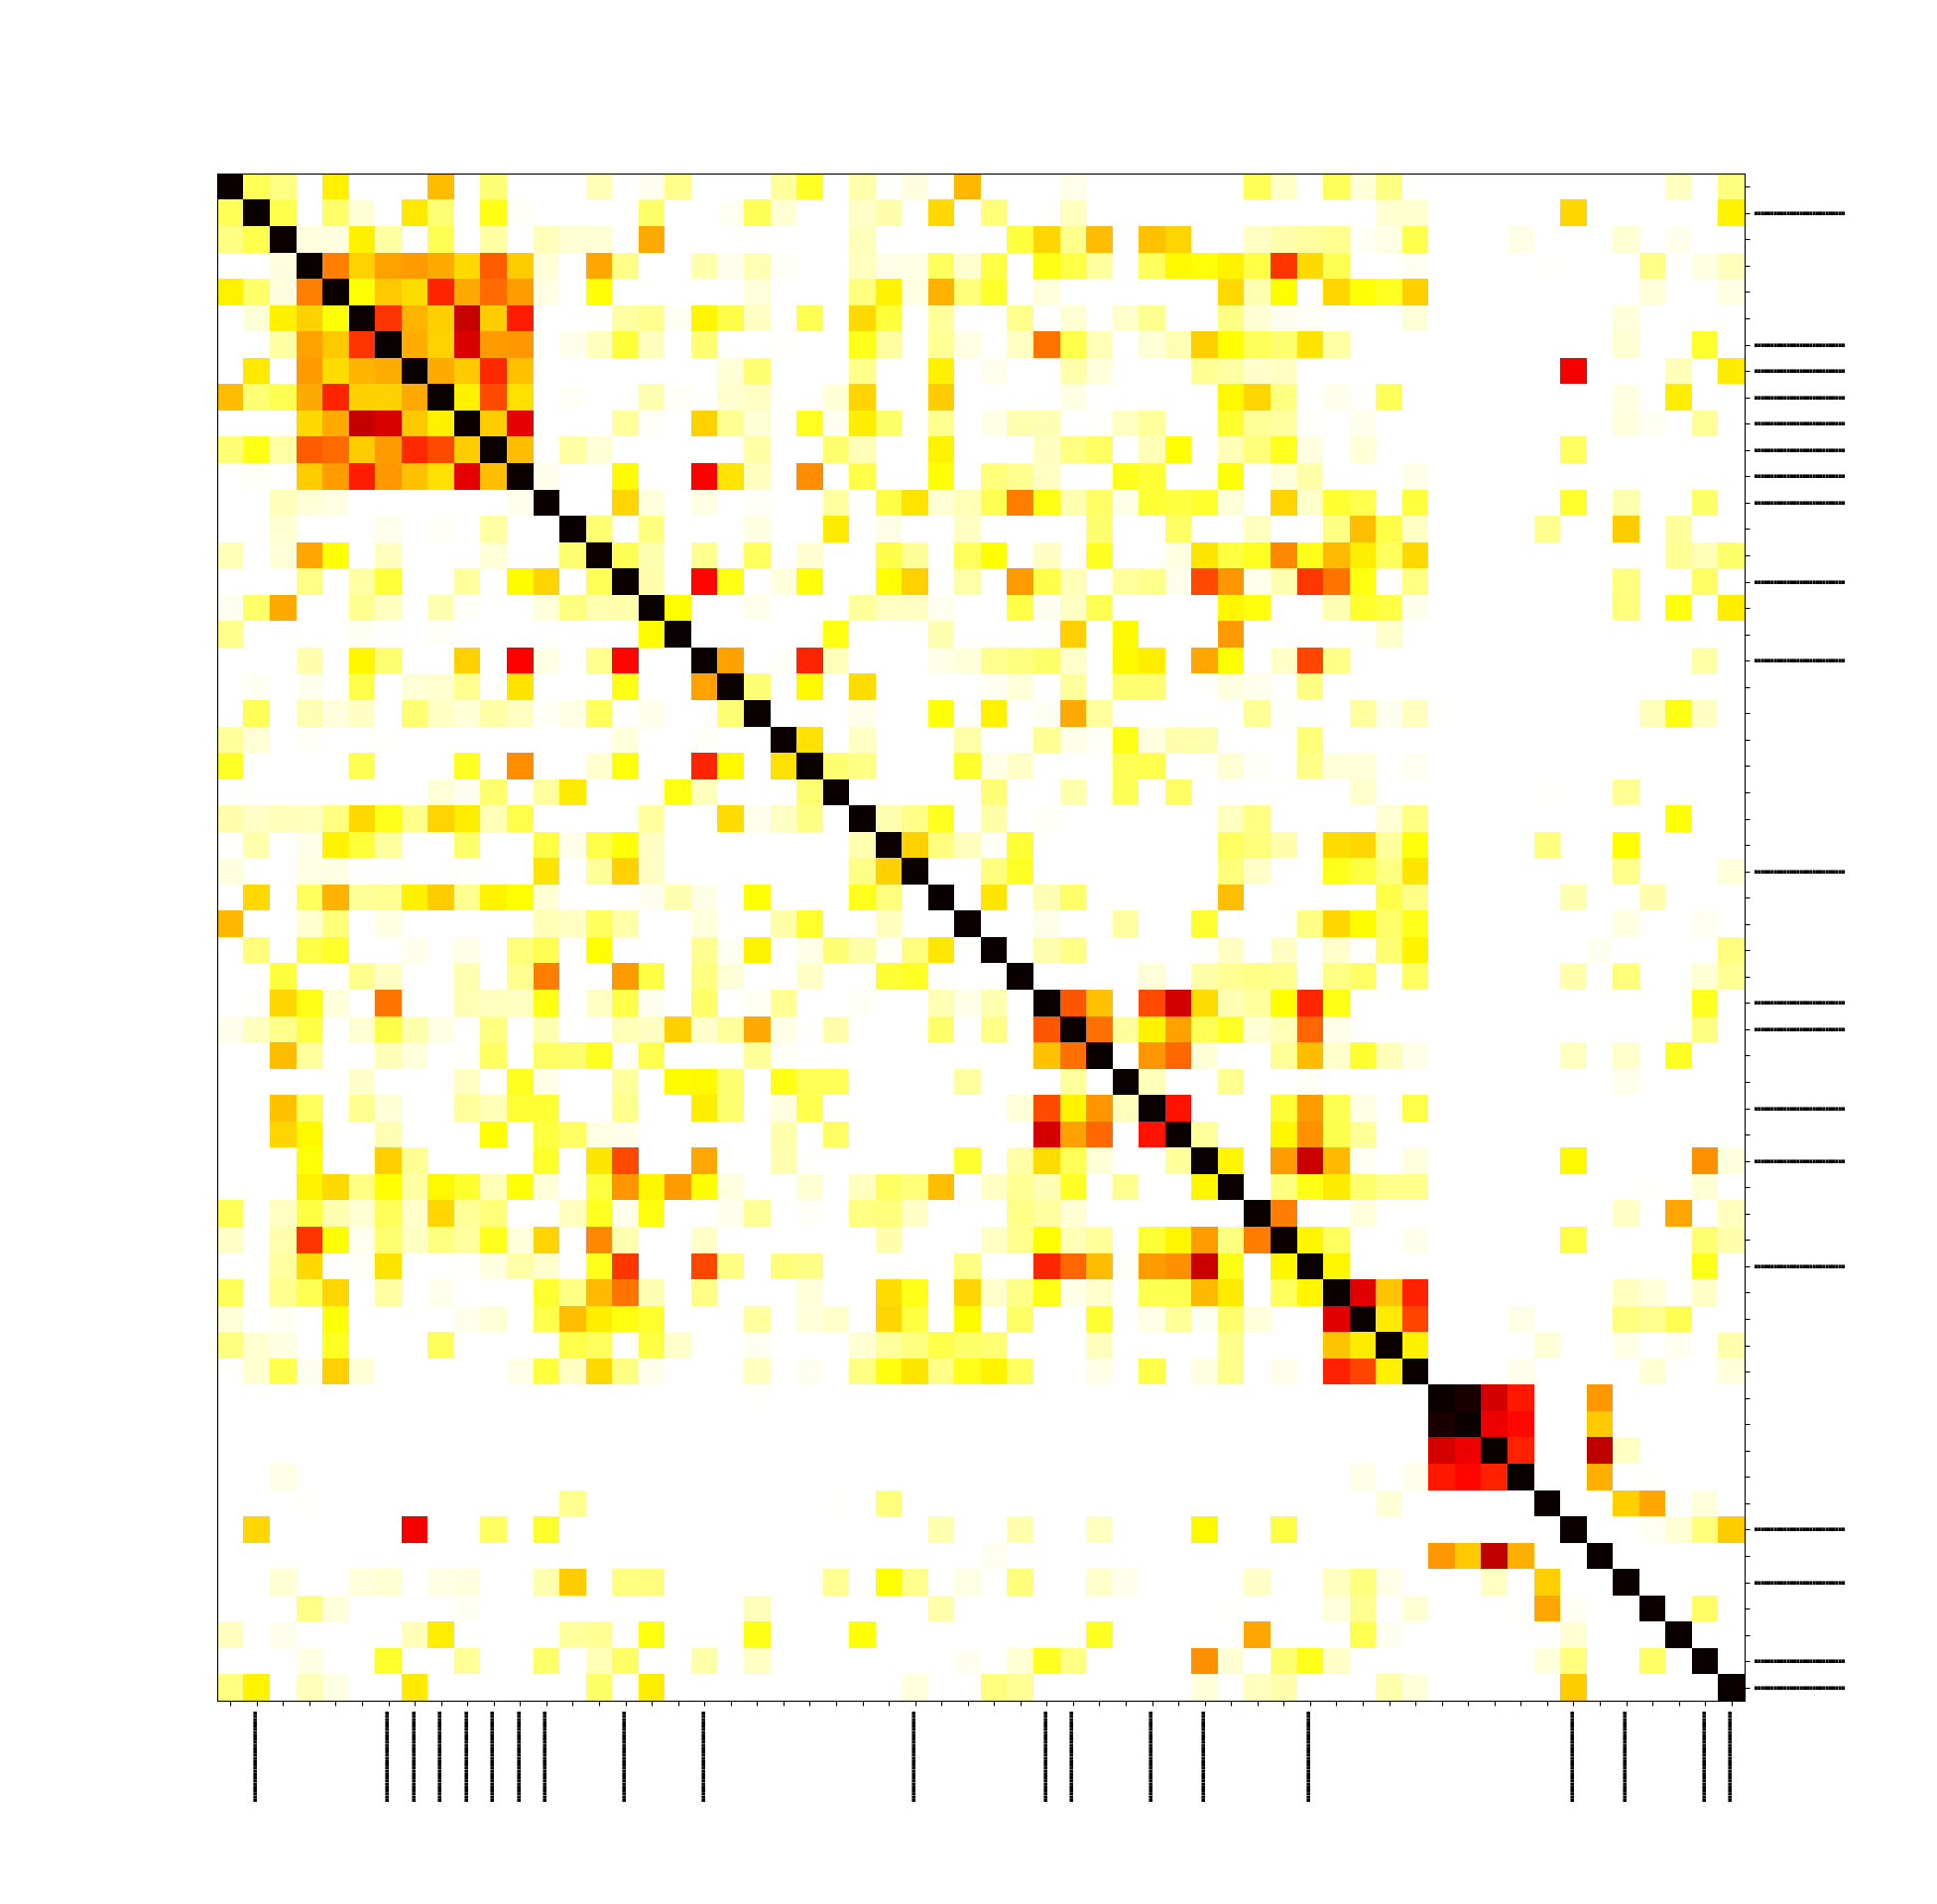
\includegraphics[width=\columnwidth]{zcash-mainnet-1543922496-fig-corr-005-txcl-003-N-Rand.png}
		\caption{Zcash, Coinomi.}
	\end{subfigure}
	\caption{Transaction clustering for mobile wallets.}
	\label{fig:clustering-all}
\end{figure}

The correlation matrices exhibit a block-diagonal structure (Figure~\ref{fig:clustering-all}), as expected.
The clusters are clearly visible for the Bitcoin wallet on testnet, for which we obtained the anonymity degree of~$0.5089$.
The adjusted anonymity degree for the Bitcoin mainnet is $0.8646$~for Bitcoin wallet, $0.8413$~for BRD, and~$0.9117$~for Coinomi.
Similar to the results with a desktop node as a transaction source, the picture for the Bitcoin mainnet is much less clear because of more transactions and nodes overall and a smaller number of connections that we establish.


\subsubsection*{Estimating the IP addresses of wallet's nodes}

Apart from clustering transactions, an adversary might be interested in obtaining the IP address of the nodes that a centralized wallet uses for transaction broadcast.
The IP address of a centralized wallet's node may not necessarily be secret.
Still, linking Bitcoin transactions with IP addresses may reveal which wallet a victim is using.
The adversary can later leverage this information for social engineering attacks.

We test this attack scenario in two experiments (Figure~\ref{fig:clustering-all}).
In the first experiment, we consider the Bitcoin testnet and Mycelium wallet.
The Mycelium transactions exhibit a clearly visible cluster: they are quickly announced from the same two IP addresses.
The time difference between these announcements is in single milliseconds.
Other nodes re-broadcast then only after tens or hundreds of milliseconds.
According to IP geolocation services, the two nodes are located in Germany (\texttt{2a01:4f9:2b:4ca::2}) and in Helsinki, Finland (\texttt{95.216.68.181}).
A reverse DNS lookup service \url{robtex.com} suggests that one of these IP addresses corresponds to a URL~\url{electrumx-b.mycelium.com}.
Both IP addresses belong to Hetzner (a cloud provider) and host Bitcoin nodes with a latency of~$25$~ms~\cite{Bitnodes}.
We estimate that each of these nodes offers more than $700$~connection slots in a separate experiment.
The second experiment considers Zcash and Coinomi wallet.
Though the Coinomi transactions do not form a clear cluster, we observe that some of them (in the second cluster) are quickly announced from the same IP (\texttt{5.79.123.194}), which, we assume, is one of Coinomi's nodes.


\subsubsection*{Comparison with prior work}

Multiple research works propose deanonymization techniques for cryptocurrencies.
However, few of them quantify their results based on ground truth data, i.e.,~by deanonymizing transactions known to have originated from one source.
For instance, one of the earliest papers~\cite{Meiklejohn2013} clusters Bitcoin transactions using transaction graph heuristics and known deanonymized addresses as a starting point.
However, it does not provide a way to verify how many of the addresses assigned, for example, to the cluster of an exchange, actually belong to it.

The same is mostly true for related work on network analysis.
As outlined in Section~\ref{sec:network-analysis}, the most closely related prior work is~\cite{Koshy2014, Biryukov2014, Neudecker2017}.
In~\cite{Koshy2014}, the first relayer heuristic is used.
However, after refining the results to eliminate likely false positives, the authors conclude that most results are based on anomalous propagation and have limited applicability.

In~\cite{Neudecker2017}, two clustering methods are compared: based on transaction graph analysis and networking analysis (first relayer heuristic with optimizations).
The authors find little correlation between the two types of clusters.
Less than $8$\% of clusters from transaction graph analysis correspond to a single IP address.
No evaluation based on the ground truth has been performed.

Only in~\cite{Biryukov2014} do the authors estimate the success using their own transactions, in addition to theoretical calculations.
They achieve a success rate of nearly $60$\% on the Bitcoin testnet, over a set of $424$~transactions.\footnote{The experiments described in~\cite{Biryukov2014} were conducted in 2014. Since then, Bitcoin Core implemented stricter rules on chains of unconfirmed transactions. The length of such chains is now restricted to $25$ by default~\cite{Daftuar2015, Morcos2015, Maxwell2016}. This limits our ability to emit a large number of transactions during one experiment. This issue does not apply to Zcash, as its source code was forked from Bitcoin~Core before the relevant changes were introduced. However, the limitation in the Zcash experiments is the time required to generate a shielded transaction (around $30$~seconds on a consumer laptop as of~2018). As of 2020, after a series of protocol optimizations, generating a shielded Zcash transaction takes $2$-$3$~seconds.}
This means that $60$\% of the testnet transaction issued from a given entry set are correctly identified as such.

Our method seems more promising since it tries to use all the available information, including timing.
In the experiment on the Bitcoin testnet (Figure~\ref{fig:bitcoin-testnet-combined}), $24$~out of $30$~control set transaction~are assigned to one cluster.
Additionally, $7$~transactions not from the control set have been put into this cluster.
Therefore, we achieve a false positive rate of $23$\% and a false negative rate of $20$\%.
This corresponds to the success rate of $80$\%, which is higher than $60$\% reported in~\cite{Biryukov2014}.

We should note however that while our method is promising, more statistical evidence is needed to quantify its advantage over previous methods precisely.


\section{Attack cost estimation}

We now estimate the resources required for a full-scale attack on the Bitcoin mainnet.
The Bitcoin mainnet consists of approximately $10\,000$~nodes reachable at any given time~\cite{Bitnodes}.
Bitcoin nodes provide $43$~connections slots on average (measured on $1\,000$~random nodes).
The size of an \texttt{inv} message is "36x + const for message with x objects"~\cite{BitcoinWiki}.
We assume that an \texttt{inv} for a single transaction requires $40$~bytes.
Bitcoin processes around $250\,000$~transactions per day (as of November~2018), or $2.89$~transactions per second.
Assuming each connection eventually relays each transaction, we arrive at the required bandwidth for one connection slot: $2.89 \times 40 = 115.6$~B/s.
A full-scale attack on the Bitcoin mainnet would require maintaining an average of~$43$~connections to $10\,000$~nodes, i.e.,~a total bandwidth of~$115.6 \times 10\,000 \times 43 = 49\,708\,000$~B/s = $47.4$~MB/s = $379$~Mbit/s.
An hour-long attack at this bandwidth will require receiving approximately $167$~GB of incoming traffic.

We estimate the attack cost based on the cost of running a full Bitcoin node.
Various estimations put that cost between $3$~and~$20$~US~dollars per month~\cite{Zeyde2018, Connell2017}.
By default, Bitcoin nodes relay transactions through $8$~outgoing connections and accepts up to $117$~incoming connections.\footnote{The experiments were performed before Bitcoin~Core introduced two more connections for block propagation. In any case, blocks are outside of the scope of our technique~\cite{Daftuar2019}.}
Assuming an average node has a total of~$125$~connection slots, $125 - 43 = 82$~slots eventually get occupied.
An adversary needs to maintain $10\,000 \times 43 = 430\,000$~connections, or approximately $5\,244$~times more than a regular node.
Considering that one month ($30$-days) is $720$~hours, we conclude that an estimated cost of an hour-long attack is approximately $5244 \div 720 = 7.3$~times the monthly cost of running a regular full node.
That leads to an estimation of bandwidth costs between $20$~and~$150$~USD\@.
The total cost of the attack is on the order of hundreds of US~dollars (taking into account the cost of computation and storage).
We conclude that the attack is well within reach of even low-budget adversaries.
All our experiments on the Bitcoin testnet and Zcash mainnet cost $35$~USD, which can likely be decreased by optimizing the scripts and storing data locally.


\section{Discussion and countermeasures}

Our technique performs well on relatively small networks (Bitcoin testnet, Zcash) and works to some extent on Bitcoin.
We expect a resourceful attacker to achieve better results on the Bitcoin mainnet by establishing more connections.

Application-level cryptographic countermeasures, such as zero-knowledge proofs in Zcash, cannot defend against our attack.
We only consider transaction hashes and their announcement times, ignoring their content.
Overlay networks such as Tor~\cite{Tor} are a popular mitigation for deanonymization attacks.
In our case, transactions announced from the same Bitcoin node would form a cluster, even if they are sent to this node through Tor.
Moreover, broadcasting transactions via Tor may introduce man-in-the-middle vulnerabilities~\cite{Biryukov2015}.

Our method's main limitation is the assumption that a user issues multiple transactions during a relatively short time frame through the same set of entry nodes (i.e.,~the same session).
Transactions issued from different sessions would not be linkable by our technique.

Practical countermeasures against transaction clustering depend on the wallet type.
For a full node that accepts incoming connections (a server):

\begin{itemize}
	\item run the node with more outgoing connections to dilute the quality of the topological fingerprint;
	\item introduce random delays on top of those implemented in the node software;
	\item drop connections to randomly chosen entry nodes and establish new ones, constantly altering the set of entry nodes;
	\item advise users not to broadcast sensitive transactions within a short period (if the node is used for broadcasting users' transactions).
\end{itemize}

Users of full nodes without incoming connections (e.g.,~behind NAT) may wish to re-launch the software to issue each transaction through a new set of entry nodes.

Proposed countermeasures for SPV nodes would be:

\begin{itemize}
	\item use wallets with P2P broadcast (e.g.,~Bitcoin wallet for Android~\cite{BitcoinWallet});
	\item if using wallets with centralized broadcast, use different wallets for transactions not meant to be linkable;
	\item connect to a trusted full node.
\end{itemize}

All users should avoid sending multiple transactions within a short time frame.

Note that an attacker may leverage external information to increase clustering accuracy, such as known addresses of exchanges and other service providers~\cite{Walletexplorer}.

\paragraph{Dandelion and Erlay}

The key property of the currently used cryptocurrency P2P protocols that we exploit is that nodes do not distinguish between incoming and outgoing connections.
A node announces transactions to a random subset of connections.
This allows a well-connected listener to receive more information by initiating more connections.
For instance, by saturating $50\%$~of a node's connection slots, a listener has a $50\%$~chance to be the first to receive a new transaction from it.

Dandelion~\cite{Fanti2018} is a P2P protocol for cryptocurrencies (see~Section~\ref{sec:Dandelion}).
It is an effective countermeasure against our attack.\footnote{The authors mention (\cite{Fanti2018}, Section~4.2) that some configurations of the protocol may be prone to transaction correlation attacks.}
In Dandelion, nodes choose neighbors for the stem phase from their outgoing connections only.
An attacker has no easy way to force a remote peer to initiate a connection.
Therefore, a malicious node with many outgoing connections does not have an advantage in the stem phase.
It can only aggregate incoming information while acting as a regular relay, gaining some but not much insight into possible transaction clusters.
The same applies to Erlay~\cite{Naumenko2019} -- a P2P protocol for a more efficient transaction broadcast in Bitcoin.


\section{Conclusion} \label{sec:Ch03Conclusion}

We have studied the state of anonymity of cryptocurrencies on the network level.
We have described and implemented a novel transaction clustering method based on the analysis of transaction announcements.
We have implemented and tested our technique on four popular cryptocurrencies using a variety of wallets.

Our results show that Bitcoin and the major privacy-focused cryptocurrencies do not sufficiently defend against network-based transaction clustering.
A low budget adversary can accurately link transactions that originate from the same node.
A similar technique allows an attacker to infer the IP addresses of nodes used for transaction broadcast by mobile wallets.
Cryptocurrencies should defend against network analysis to provide stronger privacy guarantees.
